\documentclass[11pt,letterpaper]{article}

% Compile with: xelatex main.tex; bibtex main; xelatex main.tex; xelatex main.tex
% xelatex natively understands UTF-8, no inputenc needed.

\usepackage[margin=1in]{geometry}
\usepackage{fontspec}            % xelatex font selection
\usepackage{amsmath,amssymb,amsthm}
\usepackage{graphicx}
\usepackage{float}
\usepackage{xcolor}
\usepackage{hyperref}
\usepackage[numbers,sort&compress]{natbib}
\usepackage{booktabs}
\usepackage{caption}
\usepackage{longtable}
\usepackage{array}
\usepackage{calc}
% pandoc emits \real{0.2} etc. inside table column specs; provide it.
\providecommand{\real}[1]{#1}
\providecommand{\tightlist}{\setlength{\itemsep}{0pt}\setlength{\parskip}{0pt}}
% pandoc emits \def\LTcaptype{none} to suppress table captions; define the
% counter so longtable doesn't error.
\newcounter{none}
\usepackage{microtype}
\usepackage{titlesec}
\usepackage{newunicodechar}
\usepackage{url}
% Allow line-breaks inside \url{} / \path{} at slashes, underscores,
% dots, hyphens. Output keeps typewriter font.
\PassOptionsToPackage{hyphens}{url}
% No stretchy spacing at break points — keeps path characters tight when
% the line is justified. Breaks are still enabled by \UrlBreaks below.
\Urlmuskip=0mu\relax
% Add break-points after / _ . - so file paths split cleanly.
\renewcommand{\UrlBreaks}{\do\/\do\_\do\.\do\-\do\&\do\?\do\=\do\,\do\;}
% Loosen TeX's line-breaking globally, to absorb any remaining overflow.
\sloppy
\setlength{\emergencystretch}{3em}

% Unicode -> math/text mappings (so utf8 source compiles with pdflatex)
% Greek letters
\newunicodechar{ρ}{\ensuremath{\rho}}
\newunicodechar{μ}{\ensuremath{\mu}}
\newunicodechar{σ}{\ensuremath{\sigma}}
\newunicodechar{ξ}{\ensuremath{\xi}}
\newunicodechar{α}{\ensuremath{\alpha}}
\newunicodechar{β}{\ensuremath{\beta}}
\newunicodechar{γ}{\ensuremath{\gamma}}
\newunicodechar{η}{\ensuremath{\eta}}
\newunicodechar{δ}{\ensuremath{\delta}}
\newunicodechar{ε}{\ensuremath{\varepsilon}}
\newunicodechar{τ}{\ensuremath{\tau}}
\newunicodechar{π}{\ensuremath{\pi}}
\newunicodechar{Φ}{\ensuremath{\Phi}}
\newunicodechar{Δ}{\ensuremath{\Delta}}
% Math operators / scripts
\newunicodechar{²}{\ensuremath{^{2}}}
\newunicodechar{³}{\ensuremath{^{3}}}
\newunicodechar{⁰}{\ensuremath{^{0}}}
\newunicodechar{¹}{\ensuremath{^{1}}}
\newunicodechar{⁴}{\ensuremath{^{4}}}
\newunicodechar{⁵}{\ensuremath{^{5}}}
\newunicodechar{⁶}{\ensuremath{^{6}}}
\newunicodechar{⁷}{\ensuremath{^{7}}}
\newunicodechar{⁸}{\ensuremath{^{8}}}
\newunicodechar{⁹}{\ensuremath{^{9}}}
\newunicodechar{ⁿ}{\ensuremath{^{n}}}
\newunicodechar{⁻}{\ensuremath{^{-}}}
\newunicodechar{ₑ}{\ensuremath{_{\mathrm{e}}}}
\newunicodechar{ᶜ}{\ensuremath{^{c}}}
\newunicodechar{₀}{\ensuremath{_{0}}}
\newunicodechar{₊}{\ensuremath{_{+}}}
\newunicodechar{₋}{\ensuremath{_{-}}}
\newunicodechar{√}{\ensuremath{\sqrt{\,}}}
\newunicodechar{×}{\ensuremath{\times}}
\newunicodechar{−}{\ensuremath{-}}
\newunicodechar{→}{\ensuremath{\rightarrow}}
\newunicodechar{≤}{\ensuremath{\leq}}
\newunicodechar{≥}{\ensuremath{\geq}}
\newunicodechar{≈}{\ensuremath{\approx}}
\newunicodechar{∈}{\ensuremath{\in}}
\newunicodechar{∞}{\ensuremath{\infty}}
\newunicodechar{·}{\ensuremath{\cdot}}
\newunicodechar{±}{\ensuremath{\pm}}
\newunicodechar{∝}{\ensuremath{\propto}}
\newunicodechar{∧}{\ensuremath{\wedge}}
\newunicodechar{∨}{\ensuremath{\vee}}
\newunicodechar{∑}{\ensuremath{\sum}}
\newunicodechar{≠}{\ensuremath{\neq}}
\newunicodechar{≫}{\ensuremath{\gg}}
\newunicodechar{≪}{\ensuremath{\ll}}
% Subscript Latin letters (used in symbols like h_max, J_eff, c_log)
\newunicodechar{ₐ}{\ensuremath{_{a}}}
\newunicodechar{ₓ}{\ensuremath{_{x}}}
\newunicodechar{ₖ}{\ensuremath{_{k}}}
\newunicodechar{ₘ}{\ensuremath{_{m}}}
\newunicodechar{ₚ}{\ensuremath{_{p}}}
\newunicodechar{ₛ}{\ensuremath{_{s}}}
\newunicodechar{ₜ}{\ensuremath{_{t}}}
\newunicodechar{ⱼ}{\ensuremath{_{j}}}
\newunicodechar{≳}{\ensuremath{\gtrsim}}
\newunicodechar{≲}{\ensuremath{\lesssim}}
\newunicodechar{⌊}{\ensuremath{\lfloor}}
\newunicodechar{⌋}{\ensuremath{\rfloor}}
\newunicodechar{⟨}{\ensuremath{\langle}}
\newunicodechar{⟩}{\ensuremath{\rangle}}
\newunicodechar{ℓ}{\ensuremath{\ell}}
% Punctuation
\newunicodechar{§}{\S{}}
\newunicodechar{°}{\textdegree}
\newunicodechar{…}{\ldots}
% Phonetic / IPA / specialty (best-effort fallbacks)
\newunicodechar{ˡ}{\ensuremath{^{l}}}
\newunicodechar{ˣ}{\ensuremath{^{x}}}
\newunicodechar{̄}{}
\newunicodechar{ᐟ}{}
\newunicodechar{ᴅ}{D}
\newunicodechar{ᵒ}{\ensuremath{^{o}}}
\newunicodechar{ᵢ}{\ensuremath{_{i}}}
\newunicodechar{ᵦ}{\ensuremath{_{\beta}}}
\newunicodechar{ő}{\H{o}}
% Additional glyph mappings: glyphs present in the manuscript that had no
% mapping above. Greek set in math mode -> italic for single-letter
% variables (uniform with the mapped ξ, μ, η above).
\newunicodechar{λ}{\ensuremath{\lambda}}
\newunicodechar{ζ}{\ensuremath{\zeta}}
\newunicodechar{φ}{\ensuremath{\varphi}}
\newunicodechar{½}{\ensuremath{\tfrac{1}{2}}}
\newunicodechar{Ẇ}{\ensuremath{\dot{W}}}
\newunicodechar{′}{\ensuremath{{}^\prime}}
\newunicodechar{₂}{\ensuremath{_{2}}}
\newunicodechar{ℤ}{\ensuremath{\mathbb{Z}}}
\newunicodechar{↔}{\ensuremath{\leftrightarrow}}
\newunicodechar{⇒}{\ensuremath{\Rightarrow}}
\newunicodechar{𝒩}{\ensuremath{\mathcal{N}}}

\hypersetup{
  colorlinks=true,
  linkcolor=blue!50!black,
  citecolor=blue!50!black,
  urlcolor=blue!50!black,
}

\titleformat*{\section}{\Large\bfseries}
\titleformat*{\subsection}{\large\bfseries}
\titleformat*{\subsubsection}{\normalsize\bfseries\itshape}

\setlength{\parskip}{4pt}
\setlength{\parindent}{0pt}

\title{Supplementary Information \\ \large Transient Branch Selection and Delivered Stabilizer Amplitude in a Bistable Mean-Field Model:\\ Matched-Seed Measurements of Collapse Probability}
\author{Chowon Jung\\
Department of Computer Science, University of Colorado Boulder, Boulder, Colorado, USA\\
\small\texttt{dancing4am@gmail.com}}
\date{\today}

\begin{document}
\maketitle


\renewcommand{\thesection}{S\arabic{section}}
\renewcommand{\thesubsection}{S\arabic{section}.\arabic{subsection}}
\renewcommand{\thefigure}{S\arabic{figure}}
\renewcommand{\theequation}{S\arabic{equation}}
\setcounter{figure}{0}
\setcounter{section}{0}
\setcounter{equation}{0}

\textbf{Paper:} \emph{Transient Branch Selection and Delivered Stabilizer Amplitude in a Bistable Mean-Field Model: Matched-Seed Measurements of Collapse Probability}

\textbf{Author:} Chowon Jung, Department of Computer Science, University of Colorado Boulder, Boulder, Colorado, USA.

This document supplies the technical material referenced in the main text. §S1 fully specifies the L2, L3, and L4 dynamical systems used in the ablation cascade. §S2 gives the \emph{a priori} derivation of the \emph{h}/\emph{J} scaling of Proposition 1 from the Curie--Weiss free-energy structure, together with the transient-selection derivation of the residual (§S2.7). §S3 presents Figure S1 (the L0 mean-field validation). §S4 documents the full convergence test that motivates the d\emph{t} = 0.05 choice in Methods, together with the horizon-stability check, the provenance of the headline-cell values, the boundary/clipping integrity analysis (including the boundary-preserving integrator check and the Feller classification), and the collapse-definition sensitivity grid. §S5 contains sensitivity and robustness analyses: noise prescription and \emph{h}(\emph{W}) form (§S5.1), one-at-a-time parameter sensitivity (§S5.2), alternative bistable model classes (§S5.3), the wealth-coupling coefficient \emph{h}₀ of the protective field \emph{h}(\emph{W}) = \emph{h}₀·(\emph{W}/500) required to hold P(collapse) fixed as coupling varies (§S5.4), the sensitivity of the wealth equation (§S5.5), the delivered-amplitude (magnitude-matched) controls (§S5.6), the branch-selection observable and the collapse-time decomposition of fixed-field failures (§S5.7), and the selection-formula prediction check together with the theory-derived amplitude surface (§S5.8). §S6 provides implementation details for the network agent-based model, the exact reduction of the \emph{N}-agent system to the one-dimensional SDE under the committed configuration, and the measured validity range of that reduction. §S7 contains supplementary Figure S2 (sensitivity sweep across noise prescription and \emph{h}(\emph{W}) form, supporting §S5.1), Figure S3 (scaling-vs-fixed control, supporting §S5.1), and Figure S4 (alternative-model-class robustness, supporting §S5.3 --- the asymmetry is not Curie--Weiss-specific). §S8 contains Supplementary Notes 1--8: full statements and detailed values moved from the main text during condensation (prior-work comparison; referents, Definition 1, and noise notation; delivered-amplitude control details; amplitude-requirement descriptors; late-channel and ramp detail; boundary and typing provenance; network detail; and the scope-probe statement). §S9 reports the pre-registered late-channel mechanism tests (initial-condition dependence, barrier scaling, and the waiting-time distribution).

\begin{center}\rule{0.5\linewidth}{0.5pt}\end{center}

\section{Full model specifications for the ablation cascade}\label{full-model-specifications-for-the-ablation-cascade}

This section expands the Methods description of Levels 2, 3, and 4 of the ablation cascade with the full dynamical content. Levels 0 and 1 are completely specified in the main text and are not reproduced here.

\subsection{Level 2 --- minimal model + replicator--mutator beliefs}\label{level-2-minimal-model-replicatormutator-beliefs}

Level 2 augments the L1 dynamics with a population of \emph{K} = 6 belief types competing inside each simulated system. Let \emph{f}ₖ(\emph{t}) denote the fraction of agents holding belief type \emph{k} ∈ \{0, \ldots, \emph{K} -- 1\}, with ∑ₖ\emph{f}ₖ = 1. Each belief type sits at a fixed location \emph{b}ₖ ∈ {[}--1, 1{]} on a one-dimensional opinion axis,

\[
b_k = \frac{2k - (K-1)}{K-1}, \qquad k = 0, \ldots, K-1,
\]

so that the belief axis spans the same range as the coordination order parameter \emph{m}. The replicator-mutator dynamics evolve \emph{f}ₖ between simulation steps according to

\[
f_k(t + \Delta t) = (1 - \mu_b)\,\frac{f_k(t)\,W_k(m)}{\langle W \rangle} + \frac{\mu_b}{K},
\]

with mutation rate \(\mu_{\mathrm{b}}\) = 0.01 and \emph{m}-coupled fitness

\[
W_k(m) = \exp(\gamma\,b_k\,m), \qquad \langle W \rangle = \sum_j f_j(t)\,W_j(m).
\]

The fitness coupling \emph{γ} = 1 implies that beliefs aligned with the current sign of \emph{m} are favored. The renormalization against ⟨\emph{W}⟩ keeps ∑ₖ\emph{f}ₖ = 1 to numerical precision; an additional unconditional renormalization by ∑ₖ\emph{f}ₖ at the end of each step absorbs any drift from finite-precision arithmetic.

The epistemic-coherence factor is the normalized Shannon entropy of the belief distribution,

\[
\mathrm{EC}(t) = \frac{-\sum_k f_k(t) \ln f_k(t)}{\ln K} \in [0, 1],
\]

with EC = 1 indicating uniform belief diversity and EC = 0 indicating complete monoculture. The L2 passive stabilizer field is

\[
h_{\mathrm{eff}}(t) = h(W(t)) \cdot \mathrm{EC}(t),
\]

so the operative restoring force in Equation 1 of the main text is \(h_{\mathrm{eff}}\) rather than \emph{h}. All other dynamics --- the SDE for \emph{m}, the wealth equation, and the collapse criteria --- are identical to L1.

Mechanism: at high coupling \emph{J}, the \emph{m}-coupled fitness drives the belief distribution toward whichever single type aligns with the saturated \emph{m}; EC drops toward its mutation-limited floor ≈ 0.06 (≈ 0 in pure monoculture). The passive stabilizer's effective field is then strongly attenuated even though the underlying wealth-driven \emph{h} is intact. At low \emph{J}, \emph{m} never saturates, fitness selection is weak, and EC remains high enough that \(h_{\mathrm{eff}}\) ≈ \emph{h}.

\subsection{Level 3 --- L2 + Minsky--Keen credit cycle}\label{level-3-l2-minskykeen-credit-cycle}

Level 3 adds a four-phase credit machine to the L2 dynamics. Each simulated system carries an aggregate debt state \emph{D}(\emph{t}) and a phase indicator \emph{p}(\emph{t}) ∈ \{Expansion, Euphoria, MinskyMoment, Deleveraging\}. Debt evolves continuously,

\[
\dot D = \alpha_D \cdot \max(0, m) \cdot W - \beta_D \cdot D,
\]

with debt-growth coefficient \emph{α}ᴅ = 0.5 and amortization rate \emph{β}ᴅ = 0.05. Optimism (positive \emph{m}) and high wealth fuel debt accumulation; deleveraging proceeds at a fixed rate.

Phase transitions are gated by the debt-to-wealth ratio \emph{r} = \emph{D}/max(\emph{W}, 1):

{\def\LTcaptype{none} % do not increment counter
\begin{longtable}[]{@{}
  >{\raggedright\arraybackslash}p{(\linewidth - 4\tabcolsep) * \real{0.3333}}
  >{\raggedright\arraybackslash}p{(\linewidth - 4\tabcolsep) * \real{0.3333}}
  >{\raggedright\arraybackslash}p{(\linewidth - 4\tabcolsep) * \real{0.3333}}@{}}
\toprule\noalign{}
\begin{minipage}[b]{\linewidth}\raggedright
From
\end{minipage} & \begin{minipage}[b]{\linewidth}\raggedright
To
\end{minipage} & \begin{minipage}[b]{\linewidth}\raggedright
Trigger
\end{minipage} \\
\midrule\noalign{}
\endhead
\bottomrule\noalign{}
\endlastfoot
Expansion & Euphoria & \emph{r} \textgreater{} 0.5 ∧ \emph{m} \textgreater{} 0.3 \\
Euphoria & MinskyMoment & \emph{r} \textgreater{} 1.0 \\
MinskyMoment & Deleveraging & timer ≥ 100 steps (5 physical time units at d\emph{t} = 0.05) \\
Deleveraging & Expansion & \emph{r} \textless{} 0.1 \\
\end{longtable}
}

When the MinskyMoment trigger fires, the system's wealth is reduced by 30\% (haircut), its debt is reset to zero, and the SDE noise amplitude is multiplied by 1.5 for the duration of the MinskyMoment phase. The phase-dependent income factor scales the wealth equation:

{\def\LTcaptype{none} % do not increment counter
\begin{longtable}[]{@{}ll@{}}
\toprule\noalign{}
Phase & Income factor \\
\midrule\noalign{}
\endhead
\bottomrule\noalign{}
\endlastfoot
Expansion & 1.00 \\
Euphoria & 1.10 \\
MinskyMoment & 0.50 \\
Deleveraging & 0.85 \\
\end{longtable}
}

The phase machine and the L2 belief layer evolve concurrently with the \emph{m}-SDE and the wealth equation. The L3 dynamics are completely specified by these rules together with the L2 dynamics in §S1.1.

\subsection{Level 4 --- full simulator}\label{level-4-full-simulator}

L4 is the simulator from prior work, archived in a separate repository, reachable through the Zenodo archive of this repository (concept DOI 10.5281/zenodo.20061432). L4 is prior work, not part of this deposit; no main-text claim depends on regenerating it. It comprises the L3 belief and credit dynamics together with the following additional subsystems (TypeScript implementation):

\begin{itemize}
\tightlist
\item
  \textbf{Hawkes-process shock layer} \cite{bacry2015} --- exogenous shock events with self-exciting kernel that perturb both \emph{m} and wealth at Poisson-cluster times.
\item
  \textbf{Lotka--Volterra predator--prey coupling} between an ``innovator'' and an ``imitator'' sub-population, modulating the effective income multiplier.
\item
  \textbf{Demographic dynamics} --- birth/death rates linked to wealth and age structure on the slow layer.
\item
  \textbf{Mortality} with Gompertz--Makeham hazard, coupling demographic decline to economic stress.
\item
  \textbf{Energy and infrastructure layers} with capacity dynamics that modulate consumption and noise.
\item
  \textbf{Institutional-quality slow variable} with state-dependent capacity bounds, which feeds back into \emph{h} through a fixed conversion rule (preserving Definition 1 --- the conversion is fixed even though institutional quality is dynamic).
\end{itemize}

The 16-subsystem dependency graph is DAG-validated; integration uses Strang splitting between fast/medium/slow timescales, with the fast layer integrated by an Euler--Maruyama / Heun RK2 hybrid. The L4 sweep behind the 30--35\% band cited in the main text is documented in the prior repository, reachable through the Zenodo archive of this repository (concept DOI 10.5281/zenodo.20061432).

L4 was not re-run at d\emph{t} = 0.05 for this submission; the d\emph{t} = 0.1 results from the prior repository (P(collapse) in the 30--35\% band, rigidity dominating) are consistent with the L1 → L2 → L3 trend at d\emph{t} = 0.05. A d\emph{t} = 0.05 re-run is a one-day compute task that would refine the L4 number; it is not necessary for the L1--L3 monotone claim presented in the main text.

\begin{center}\rule{0.5\linewidth}{0.5pt}\end{center}

\section{Full derivation of Proposition 1}\label{full-derivation-of-proposition-1}

This section derives the \emph{h}/\emph{J} scaling claim of Proposition 1 from the mean-field free-energy structure of Equation 1. We work in the deterministic limit first (§S2.1--§S2.4), then add the multiplicative noise contribution (§S2.5) and state the noise-corrected form (§S2.6); §S2.7 then derives the observed residual as transient branch selection at the unstable origin and validates it against the simulator.

\subsection{Effective potential}\label{effective-potential}

The deterministic part of Equation 1 can be written as a gradient flow,

\[
\dot m_{\mathrm{det}} = -\frac{\partial V}{\partial m},
\]

with effective potential (free-energy analogue)

\[
V(m;\,J,h,T) = \frac{m^2}{2} - \frac{T}{J}\ln\cosh\!\left(\frac{Jm + h}{T}\right) + C(J, h, T).
\]

The constant \emph{C} fixes the zero of \emph{V} and plays no role in the dynamics. Taking the derivative reproduces

\[
-\frac{\partial V}{\partial m} = -m + \tanh\!\left(\frac{Jm + h}{T}\right),
\]

confirming the gradient form. The fixed points of the deterministic dynamics are the critical points of \emph{V}.

\subsection{Fixed-point structure}\label{fixed-point-structure}

Critical points satisfy


\begin{equation*}
m = \tanh\!\left(\frac{Jm + h}{T}\right). \tag{S1}
\end{equation*}


For \emph{h} = 0, Equation S1 is the standard Curie--Weiss self-consistency equation. It has a single stable solution \emph{m} = 0 for \emph{J} \textless{} \emph{T} and three solutions for \emph{J} \textgreater{} \emph{T}: two stable branches at \emph{m} = ±\emph{m}* and an unstable saddle at \emph{m} = 0, with \emph{m}*(\emph{J}, \emph{T}) → 1 as \emph{J} / \emph{T} → ∞.

The bifurcation at \emph{J} = \emph{T} is the Curie--Weiss critical point. We write \emph{J}ᶜ = \emph{T} below.

\subsection{\texorpdfstring{Asymmetric splitting under \emph{h} \textgreater{} 0}{Asymmetric splitting under h \textgreater{} 0}}\label{asymmetric-splitting-under-h-0}

For \emph{h} \textgreater{} 0 and \emph{J} ≫ \emph{T}, all three critical points persist but shift. Writing \emph{m} = 1 -- ε with ε \textgreater{} 0 small for the upper branch, substituting into Equation S1, and using the asymptotic tanh(\emph{x}) = 1 -- 2 e⁻²ˣ + \emph{O}(e⁻⁴ˣ) yields


\begin{equation*}
\varepsilon_+ \approx 2\,\exp\!\left(-\frac{2(J + h)}{T}\right). \tag{S2}
\end{equation*}


The same calculation for \emph{m} = --1 + δ gives


\begin{equation*}
\delta_- \approx 2\,\exp\!\left(-\frac{2(J - h)}{T}\right). \tag{S3}
\end{equation*}


Both branches are exponentially close to ±1 for \emph{J} ≫ \emph{T}, and the splitting between ε₊ and δ₋ is exponentially small in 2\emph{h}/\emph{T}. The saddle, by contrast, sits at \emph{m}ₛ = --\emph{h}/(\emph{J} -- \emph{T}) ≈ --\emph{h}/\emph{J} for \emph{J} ≫ \emph{T}; the linear-in-\emph{h} shift of the saddle along the \emph{m} axis is the basic geometric fact behind the asymmetry.

\subsection{\texorpdfstring{Barrier height and the \emph{h}/\emph{J} ratio}{Barrier height and the h/J ratio}}\label{barrier-height-and-the-hj-ratio}

The barrier between the two branches is

\[
\Delta V_{\text{barrier}} = V(m_s) - \min(V(m_+), V(m_-)).
\]

For \emph{J} ≫ \emph{T} and \emph{h} = 0, evaluating \emph{V} at the symmetric fixed points and the saddle gives the standard Curie--Weiss expression


\begin{equation*}
\Delta V_{\text{barrier}} = \frac{1}{2} - \frac{T}{J}\ln 2 + \mathcal{O}\!\left(e^{-2J/T}\right) \xrightarrow{J \gg T} \frac{1}{2}. \tag{S4}
\end{equation*}


The barrier approaches a finite ceiling of ½ for \emph{J} ≫ \emph{T} (in the same V-units as the tilt); it does not grow with \emph{J}.

The \emph{h} \textgreater{} 0 perturbation tilts the landscape between the two branches. From §S2.3, the asymmetric energy splitting between the protective and unprotective branches is


\begin{equation*}
\Delta V_{\text{tilt}} = V(m_-) - V(m_+) \approx \frac{2 h\,m_*}{J} \approx \frac{2 h}{J} \tag{S5}
\end{equation*}


for \emph{J} ≫ \emph{T}, since \emph{m}* → 1. Note that the tilt \textbf{scales as \emph{h}/\emph{J}} --- the tilt itself decreases with coupling, even though \emph{h} is fixed.

The dimensionless quantity controlling the passive stabilizer's ability to bias the equilibrium probabilities of the two branches is the ratio of tilt to barrier:


\begin{equation*}
\eta(J, h, T) \equiv \frac{\Delta V_{\text{tilt}}}{\Delta V_{\text{barrier}}} \approx \frac{2h/J}{1/2} = \frac{4h}{J}\bigl[1 + \mathcal{O}(T/J)\bigr] \xrightarrow{J \gg T} \mathcal{O}\!\left(\frac{h}{J}\right). \tag{S6}
\end{equation*}


This is Proposition 1's central statement: the tilt-to-barrier ratio --- the deterministic preferential pull toward the protective branch relative to the barrier separating the branches --- \textbf{scales as \emph{h}/\emph{J}} at high coupling. Within the committed parameterization, \emph{h}(\emph{W}) = 2(\emph{W}/500) is bounded above by the equilibrium wealth, itself bounded by the static parameter \emph{μ} through Equation 2 of the main text, so \emph{η} → 0 as \emph{J} → ∞ for any fixed \emph{μ}. This is an asymptotic property of the ratio \emph{η} within the model; what it implies for collapse probabilities at \emph{finite} coupling is an empirical question, answered by the measured comparison of the specified parameterizations (main text; §S5.1): there, fixed fields \emph{h} = 2.4 and 5.0 hold P(collapse) ≤ 0.001 at \emph{μ} = 100 throughout the calibrated range \emph{J} ≤ 5 (0.00 at \emph{n} = 100; 0.001 at \emph{n} = 1,000, §S5.7), so boundedness alone does not determine finite-\emph{J} outcomes. (In the static sweeps every wealth-fed variant delivers a field profile built on the base 2(\emph{W}/500), differing in delivered field-amplitude \emph{profile}; whether any single summary of that profile orders the outcomes is examined in §S5.6 as an exploratory, domain-dependent question, not advanced as a result.)

\subsection{Multiplicative-noise correction}\label{multiplicative-noise-correction}

The full SDE in Equation 1 of the main text adds a multiplicative noise term

\[
\xi\,\sqrt{1 - m^2}\,\zeta(t),
\]

(\emph{ζ}(\emph{t}): the white noise of Equation 1 of the main text, written \emph{ζ} here --- as in §S2.7 --- to avoid clash with the tilt-to-barrier ratio \emph{η} of §S2.4), which vanishes at the saturated branches \emph{m} = ±1. This has two effects.

First, the equilibrium measure of the SDE is \textbf{not} the Boltzmann measure of \emph{V} alone. The Itô-form Fokker--Planck equation,

\[
\partial_t P = -\partial_m\!\left[\left(-\partial_m V\right) P\right] + \frac{1}{2}\partial_m^2\!\left[\xi^2 (1 - m^2) P\right],
\]

has steady-state solution proportional to (after multiplying out)

\[
P_{\mathrm{ss}}(m) \propto \frac{1}{\xi^2(1 - m^2)}\exp\!\left(-\frac{2}{\xi^2}\,U_{\mathrm{eff}}(m)\right), \qquad U_{\mathrm{eff}}(m) = \int^m \frac{\partial_m V(m')}{1 - {m'}^2}\,dm'.
\]

Near the saturated branches the prefactor 1/(1 -- \emph{m}²) diverges, reflecting the fact that the noise is suppressed there and the trajectories spend exponentially long times in the immediate neighborhood of ±1. The \emph{exponentially weighted} probability mass on each branch is governed by \(U_{\mathrm{eff}}\), not \emph{V}.

Second, the steady-state preference between branches is controlled by the \emph{difference} of the effective potential, ΔU = \(U_{\mathrm{eff}}\)(\emph{m}₋) − \(U_{\mathrm{eff}}\)(\emph{m}₊). Rather than asserting (as an earlier draft did) that the multiplicative-noise prefactors ``cancel'' to leading order, we compute this difference explicitly (parameter-free; script \protect\path|simulation/scripts/phase1b_noise_leg.py|). Two facts hold to leading order for \emph{J} ≫ \emph{T}. (i) \emph{The multiplicative-noise tilt equals the deterministic tilt.} Quadrature of ΔU between the interior wells gives ΔU/ΔV → 1 and \emph{J}·ΔU/\emph{h} → 2 as \emph{J} grows (both ΔU and ΔV ≈ 2\emph{h}/\emph{J}), so the \emph{h}/\emph{J} scaling is \textbf{prescription-independent}, with an \emph{O}(\emph{T}/\emph{J}) remainder (e.g.~ΔU/ΔV = 1.33, 1.08, 1.01 at \emph{J} = 4, 8, 20). (ii) \emph{The wells are exponentially pinned at ±1.} The field-sensitivity of the well location d\emph{m}₊/d\emph{h} tracks \(e^{-2J/T}\) (verified: 4.4 × 10⁻² → 3.7 × 10⁻⁹ as \emph{J} = 4 → 20, matching \(e^{-2J/T}\)), so the multiplicative prefactor and the boundary-layer concentration are \emph{h}-insensitive up to \(O(e^{-2J/T})\) and \textbf{cannot} enter the leading \emph{h}/\emph{J} tilt --- replacing the hand-waved cancellation with this explicit suppression. What we do \textbf{not} establish is a rigorous error bound on the full Itô stationary \emph{occupation ratio}, whose \emph{O}(1) Kramers prefactor near ±1 remains numerically delicate (the quadrature ratio drifts ≈ 13\%--45\% over \emph{J} = 3.5--6 as the 1/(1 − \emph{m}²) factor enters); only the leading \emph{h}/\emph{J} exponent of the inter-branch tilt is secured. For this reason the result below is stated as a \textbf{Proposition} --- asymptotic \emph{h}/\emph{J} scaling of the inter-branch tilt, regime \emph{J} ≫ \emph{T}, leading order --- rather than a theorem.

\subsection{\texorpdfstring{Statement of Proposition 1 and what \emph{h}/\emph{J} governs}{Statement of Proposition 1 and what h/J governs}}\label{statement-of-proposition-1-and-what-hj-governs}

Combining §S2.4 and §S2.5: the dimensionless tilt-to-barrier ratio between the protective branch and the unprotective branch, in the deterministic mean-field limit,

\[
\eta(J, h, T) = \frac{4 h}{J}\bigl[1 + \mathcal{O}(T/J) + \mathcal{O}(\xi^2)\bigr],
\]

vanishes as \emph{J} → ∞. This is the formal content of Proposition 1.

It is important to specify what physical observable this ratio governs. \emph{η} is the ratio of the energy \emph{tilt} between branches (\(\Delta{}V_{\mathrm{tilt}}\) ≈ 2\emph{h}/\emph{J}) to the \emph{barrier} separating them (\(\Delta{}V_{\mathrm{barrier}}\) → ½ for \emph{J} ≫ \emph{T}, in the same V-units as the tilt). Two things follow.

\begin{enumerate}
\def\labelenumi{(\roman{enumi})}
\item
  \emph{Landscape topology.} When \emph{η} approaches unity from below, the tilt is comparable to the barrier and one of the two wells flattens or disappears. \emph{η} → 0 means the two wells survive and become energetically symmetric: at fixed \emph{h}, the wrong-branch attractor persists at sufficiently high coupling, because eliminating the second well requires a tilt comparable to the barrier (\emph{η} ≳ 1). This is a statement about the landscape topology of the potential, not by itself a statement about measured collapse rates: in the simulations, the fixed fields \emph{h} = 2.4 and 5.0 hold P(collapse) ≤ 0.001 at \emph{μ} = 100 throughout the calibrated range \emph{J} ≤ 5 (0.00 at \emph{n} = 100; 0.001 at \emph{n} = 1,000, §S5.7; §S5.1), and the stress form (the one variant whose field responds within a run to \emph{m}) and the coupling form suppress the residual to ≤ 0.05 at \emph{α} ≥ 0.5 and eliminate it at the tested \emph{α} = 1.0 and 2.0, while the quadratically coupling-responsive form retains a 0.14 residual at \emph{α} = 1.0 (§S5.1) --- an unbounded functional form alone is not sufficient. In static sweeps the coupling and quadratic variants deliver per-\emph{J} constant rescalings of the wealth-fed base field 2(\emph{W}/500), while the stress form adds a within-run state response (α·max(0, −\emph{m})·\emph{J}); §S5.6's exploratory ordering test of whether any single summary of the delivered field orders the variants is domain-dependent and yields no refutation under the domain rule the paper adopts. At the fully-stabilized headline coefficient \emph{α} = 2.0 the stress variant and a matched constant are both at P = 0.00 --- an all-zero consistency check that cannot discriminate form from magnitude. At an informative operating point (\emph{α} = 0.05, §S5.6, control E2) a constant matched to the active form's full-trajectory delivered mean collapses far \emph{less} than the active form itself (verdict REFUTED in all three cells), because for constant and rescaled fields, at fixed \emph{J}, the full-trajectory delivered mean is not a sufficient statistic for the outcome (E2) --- so for the coupling and quadratic variants the suppression thresholds above are statements about delivered field-amplitude profiles during the selection window, while the stress form's suppression is carried by its rectified response (§S5.8), not by within-run responsiveness of a rescaled field.
\item
  \emph{Stationary branch occupation.} In Kramers theory \cite{hanggi1990} the ratio of occupation times between branches is exp(\(\Delta{}V_{\mathrm{tilt}}\)/σ²) where σ² is the effective noise variance. Substituting \(\Delta{}V_{\mathrm{tilt}}\) = 2\emph{h}/\emph{J} gives an exponent ∝ \emph{h}/\emph{J} --- the same \emph{h}/\emph{J} scaling carried by the tilt-to-barrier ratio \emph{η} of §S2.4. Both the deterministic ratio and the additive-noise Kramers exponent therefore share the same leading \emph{h}/\emph{J} dependence. For weak noise (\emph{ξ} small) any tilt above σ² produces strong occupation preference; the effect of high coupling on the steady-state population is mediated through the \emph{h}/\emph{J} exponent in this regime.
\end{enumerate}

What our simulation reports --- the residual collapse rate at high \emph{J} --- is determined primarily by \emph{initial branch selection} under multiplicative noise that vanishes at saturation, rather than by asymptotic stationary occupation. Initial selection is symmetric when basins are narrow (high \emph{J}), and once an unlucky trajectory lands on the −\emph{m} branch the noise \(\xi \sqrt{1-m^2}\) prevents escape. The asymmetry shrinks at high coupling because the origin-instability rate \emph{λ} grows with \emph{J} while the transient bias \emph{c} is pinned at the selection-window field, leaving the bias less time to act (§S2.7). The scaling of the \emph{observed} residual collapse rate with \emph{J} is derived in §S2.7 as transient branch selection at the unstable origin and characterized empirically in §S5; it does \emph{not} share η's leading exponent.

Both the deterministic tilt-to-barrier ratio and the additive-noise Kramers occupation exponent carry the same leading \emph{h}/\emph{J} dependence; the corrected derivation therefore does not support the earlier suggestion of a prescription-dependent exponent (\emph{h}/\emph{J}² versus \emph{h}/\emph{J}). The multiplicative-noise prescription shifts the \emph{O}(1) prefactor and the initial-branch-selection weighting, not this leading exponent. The qualitative finding --- that the inter-branch tilt of a fixed field shrinks as \emph{h}/\emph{J} while the barrier stays \emph{O}(1) --- is robust to the noise prescription; how this translates into measured collapse probabilities for specific parameterizations is quantified in §S5.1 and §S5.4.

\subsection{The residual as selection at the unstable origin (Suzuki transient selection)}\label{the-residual-as-selection-at-the-unstable-origin-suzuki-transient-selection}

§S2.6 established that the \emph{observed} residual is set by \textbf{initial branch selection} rather than stationary occupation, and deferred its \emph{J}-dependence to empirics. Here we derive that dependence in closed form and validate it against the simulator.

\textbf{Regime (precondition).} This subsection applies in the common-mode regime, in which the order parameter carries aggregate \emph{O}(1) noise. Under purely idiosyncratic noise with large \emph{N} the macroscopic fluctuation is ∝1/\(\sqrt{N}\), no escape occurs, and the residual vanishes (§S6); the \emph{J}-dependence below is conditional on the common-mode regime, not independent of it.

\textbf{Why selection, not Kramers escape.} At the good well the wealth feedback drives \emph{W} to its high fixed point (\emph{W} → 3500 at \emph{μ} = 100), so \emph{h} = 2(\emph{W}/500) → 14 and \emph{η} = 4\emph{h}/\emph{J} is large; steady-state escape from the good well is negligible. Collapse is decided in the \textbf{initial transient} from (\emph{m} = 0, \emph{W} = 100), where the transient field is \(h_{\mathrm{eff}}\) = \emph{h}(\emph{W}₀) = 0.4. Numerically the median collapse occurs within 1.4--1.7\% of the run horizon across \emph{J} --- collapses are early-transient, confirming selection.

\textbf{Linearization and the wrong-branch probability.} For \emph{h} \textgreater{} 0 the point \emph{m} = 0 is not a fixed point: \emph{f}(0) = tanh(\(h_{\mathrm{eff}}\)/\emph{T}) \textgreater{} 0. Linearizing the drift,

\[
\dot m = \lambda m + c + \xi\,\zeta(t), \quad c = \tanh(h_{\mathrm{eff}}/T), \quad \lambda = -1 + (J/T)\,\mathrm{sech}^2(h_{\mathrm{eff}}/T),
\]

with ζ the common-mode unit white noise (the model's multiplicative noise \(\xi \sqrt{1-m^2}\) reduces to additive ξ at the origin to leading order in \emph{m}, where the branch is selected). For \emph{J} \textgreater{} \emph{T}·cosh²(\(h_{\mathrm{eff}}\)/\emph{T}) ≈ 2.08 the origin is \textbf{linearly unstable} (λ \textgreater{} 0) --- Suzuki's selection at an unstable point \cite{suzuki1977,mckanetarlie2001}, a mechanism experimentally confirmed in the transient decay of optically unstable states \cite{arecchipoliti1980}. Integrating, the eventual sign of \emph{m} (good + vs collapse − branch) is fixed by the effective seed \emph{Z} = \emph{c}/λ + 𝒩(0, ξ²/2λ), so the collapse probability is

\[
P_{\mathrm{coll}}(J) = \Phi\!\left(-\frac{c}{\xi}\sqrt{\frac{2}{\lambda(J)}}\right),
\]

with Φ the standard normal CDF. Three consequences: (a) \textbf{ceiling → ½} as \emph{J} → ∞ (λ → ∞ ⇒ argument → 0): an infinitely fast instability leaves the bias no time to act, so selection becomes a coin flip and the closed-form collapse probability saturates at a ½ ceiling (an asymptotic statement; see item (b) of the deepened characterization below for what the simulated range can and cannot pin); (b) \textbf{monotone} increase in \emph{J}; (c) \textbf{no power law} --- \emph{P} is a Gaussian CDF of a function \(\propto \lambda(J)^{-1/2}\), λ affine in \emph{J}, so any power-law fit returns a window-dependent effective exponent.

\textbf{Numerical validation (parameter-free).} With \emph{c}, λ(\emph{J}), ξ fixed by the committed constants (\emph{T} = 2, ξ = 0.5, \(h_{\mathrm{eff}}\) = 0.4) --- no fitted parameters --- the prediction matches the simulated passive residual at \textbf{R² = 0.93, MAE = 0.024} across \emph{J} ∈ {[}2.5, 20{]} (a conservative window: it includes the low-\emph{J} points that honesty flag (i) below notes are over-predicted, so the reported R² understates the agreement; the fit is near-exact for \emph{J} = 4--7). The pre-registered α-fit's target was the efficacy ratio E(\emph{J}) = 1 − P(\emph{J}, 100)/P(\emph{J}, 40), fitted against (\emph{J} − 2)\^{}(−\emph{α}): point estimate 0.63 (bootstrap SE 0.10, 95\% CI {[}0.53, 0.93{]}); its pre-declared SE ≤ 0.05 stopping target was not reached at the 800-seed cap, and its pre-declared \emph{n} = 5 subsample fit had CI {[}−0.46, 2.38{]}, spanning both ½ and 1 (protocol archived at \protect\path|simulation/prereg/PREREG_alpha_fit_2026-05-30.md|). The closed form's window-dependent local slope --- ≈2.2 in a low-\emph{J} window, ≈0.35 at high \emph{J}, ≈0.69 over the full range --- explains why neither E(\emph{J}) nor P(\emph{J}, 100) admits a single exponent; the full-range ≈0.69 and the measured 0.63 are slopes of \emph{different} functions, not a numerical reproduction of one by the other (on the measurement grid the log--log slope of P(\emph{J}, 100) is +1.26). The α-fit thus measured the local slope of a saturating selection CDF, not a power law; this \textbf{connects} the measured residual to the same model --- accounting for the §S2.6 gap between the theory and its observable --- while making explicit that the residual is governed by the transient instability rate λ, distinct from the stationary η = \emph{h}/\emph{J} (it does \emph{not} share η's exponent, §S2.6). This separation between a transient rate that governs the response to a shock and the stationary barrier that governs steady-state stability mirrors the stability--resilience distinction documented for early-warning indicators in bistable systems \cite{daikorolevgore2015}. Validation script: \protect\path|simulation/scripts/suzuki_selection_validation.py|.

\textbf{Suzuki↔Kramers crossover.} The two pictures are separated in \emph{time}: early transient selection (Suzuki) sets the residual, while the late deep-well regime (Kramers over a large \emph{η}-barrier) contributes negligibly. This crossover, with the near-symmetric small-\emph{h} limit where Suzuki scaling carries logarithmic corrections, further smears any single exponent.

\textbf{Honesty flags.} (i) The linearization holds for λ not too small; as \emph{J} → \emph{T} (λ → 0) the selection time diverges and the leading-order formula over-predicts (e.g.~\emph{J} = 3), so we do not extrapolate below \emph{J} ≈ 3.5. (ii) The bias uses the transient field \(h_{\mathrm{eff}}\); \emph{W} (hence \emph{h}) grows modestly during the brief selection window, which is why slow (low-\emph{J}) selection is mispredicted while fast (high-\emph{J}) selection is near-exact --- an approximation we state rather than hide. (iii) This is Suzuki's 1977 selection theory together with Kramers escape \emph{applied} to a controller-failure setting, not new mathematics.

\textbf{Deepened characterization of the transient-selection mechanism.} Three consequences of the closed form \(P_{\mathrm{coll}}\)(\emph{J}) = Φ(−(\emph{c}/\emph{ξ})\(\sqrt{2/\lambda}\)) sharpen ``no clean exponent'' from an observation into a mechanistic statement (parameter-free; script \protect\path|simulation/scripts/phase1a_suzuki_deepen.py|). (a) \emph{Continuous local exponent.} The local slope \(a_{\mathrm{loc}}\)(\emph{J}) = d ln \(P_{\mathrm{coll}}\)/d ln \emph{J} is not constant: it sweeps \textbf{6.40 → 0.10} across \emph{J} = 2.5 → 20 with no plateau, equaling \textbf{0.73} at \emph{J} ≈ 4. A windowed power-law fit therefore returns whatever \(a_{\mathrm{loc}}\) averages over its window --- which is exactly why the pre-registered fit returned an ambiguous exponent (point estimate \textbf{0.63}, 95\% CI {[}0.53, 0.93{]}; its window centers near \emph{J} ≈ 4): there is no power law to measure, only the local slope of a saturating selection CDF. (b) \emph{Approach to the ½ ceiling} (closed form): (½ − \(P_{\mathrm{coll}}\)) \(\propto J^{-1/2}\) as \emph{J} → ∞ (log-log slope −0.50; \((\tfrac{1}{2} - P_{\mathrm{coll}})\sqrt{J} \to 0.32 = \varphi(0)\,(c/\xi)\,\sqrt{2T/\operatorname{sech}^2(h_{\mathrm{eff}}/T)}\)). This is a \emph{closed-form} property: the 800-seed simulator reaches only \emph{J} = 50 --- far below the \emph{J} \textasciitilde{} 10³ onset of the asymptote --- so the (noisy, non-monotone) simulated residual is consistent with approach to ½ but does \textbf{not} pin the −1/2 exponent. (c) \emph{Noise structure sets the failure mode, not the selection probability.} Because the branch is chosen at the origin where \(\sqrt{1-m^2}\) → 1, the selection \emph{probability} is noise-structure-invariant \textbf{only for fast selection} (\emph{J} ≥ 6: additive vs multiplicative agree to ≈ 0.02--0.04); near threshold (\emph{J} ≈ 3--4) slow selection lets \emph{m} wander where \(\sqrt{1-m^2}\) \textless{} 1 and the two differ by a factor ≈ 2--3. What the noise structure robustly fixes is the \emph{failure type} (multiplicative noise vanishing at ±1 locks trajectories in → rigidity; additive noise admits fragmentation; §S5.1), not the leading selection probability.

\begin{center}\rule{0.5\linewidth}{0.5pt}\end{center}

\section{Supplementary Figure S1 --- L0 mean-field validation}\label{supplementary-figure-s1-l0-mean-field-validation}



\begin{figure}[H]
\centering
\renewcommand{\figurename}{Supplementary Figure}
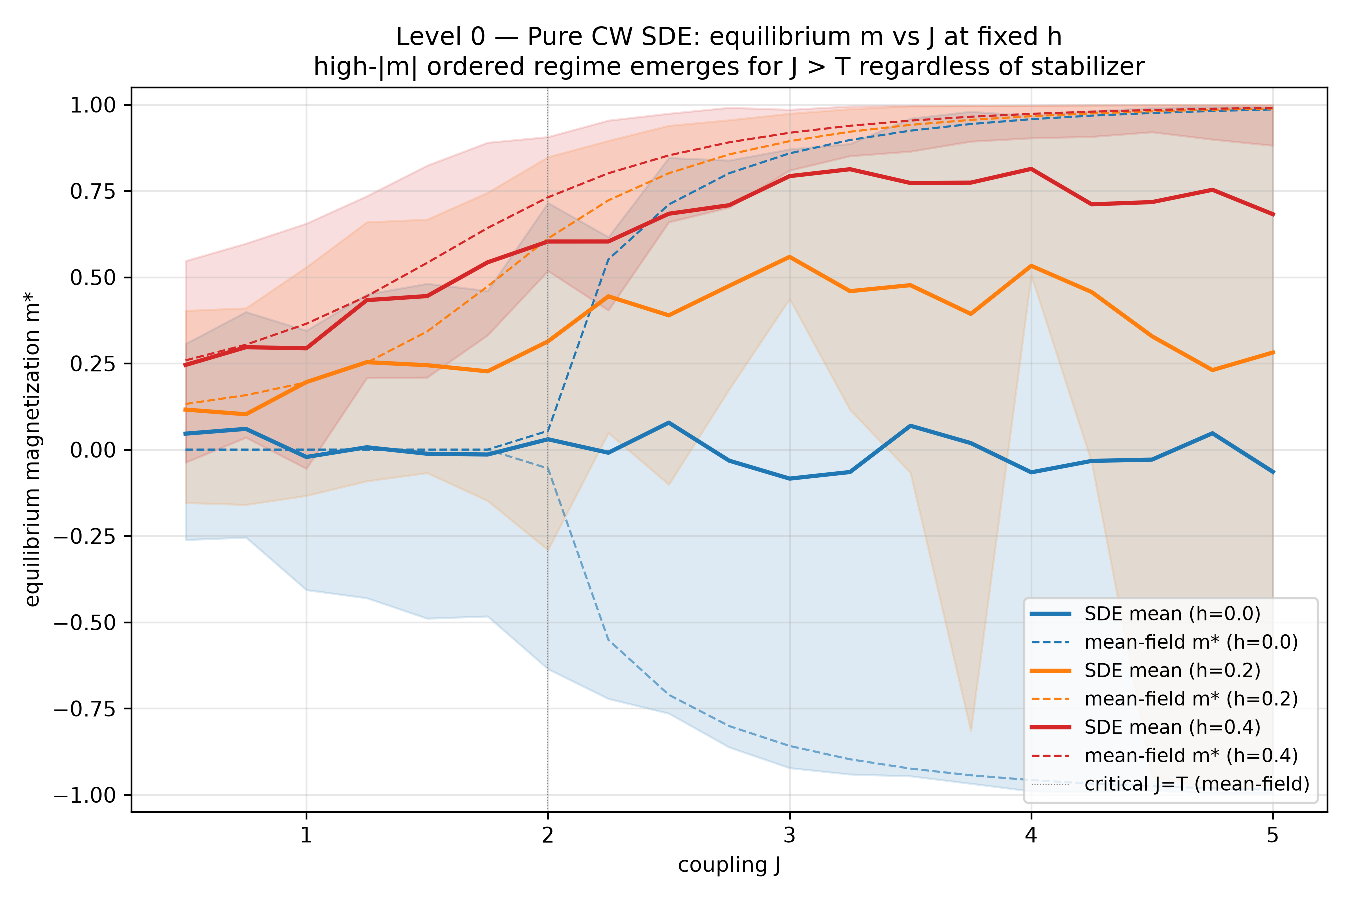
\includegraphics[width=0.95\textwidth]{figures/figS1.pdf}
\caption{\textit{Mean-field equilibrium curves for the bare Curie--Weiss SDE (Level 0).} The figure shows the long-time mean of independent SDE trajectories at each (\emph{J}, \emph{h}) cell, with \emph{h} held fixed at three values (\emph{h} ∈ \{0.0, 0.2, 0.4\}) and \emph{J} swept across \{0.5, \ldots, 5.0\}. Dashed curves are the analytical mean-field fixed points obtained by solving Equation S1 numerically; solid colored curves are the SDE long-time means with shaded bands showing the interquartile range across seeds. For \emph{h} \textgreater{} 0 (orange and red), the SDE cross-seed mean tracks the upper mean-field branch at low coupling but falls increasingly below it as \emph{J} rises (e.g.~at \emph{h} = 0.2 the mean is ≈ 0.23 against an upper branch ≈ 0.99 by \emph{J} ≈ 4.75). This is not a breakdown of the mean-field description but the finite-noise residual-selection effect central to this paper: a fraction of seeds are noise-selected onto the lower (--\emph{m}) branch (the lower quartile reaches ≈ --0.95 at high \emph{J} while the upper quartile continues to track the upper branch), dragging the cross-seed average down. For \emph{h} = 0 (blue), the SDE mean fluctuates around zero --- an expected finite-sample effect under spontaneous symmetry breaking, where individual seeds lock onto either the +1 or --1 branch and the cross-seed average cancels --- while the mean-field curves plotted show both symmetric branches. This validates the analytical backbone of Proposition 1: the mean-field free-energy structure used to derive the \emph{h}/\emph{J} scaling in §S2 is the correct effective description of the bare SDE in the absence of the wealth--field coupling, modulo the finite-sample symmetry-breaking caveat at \emph{h} = 0 which does not affect Proposition 1 (which applies for \emph{h} ≠ 0). Source file: \protect\path|simulation/results/ablation/level0_equilibrium_curves.png|; rendered here as Supplementary Figure S1, \protect\path|manuscript/arxiv/figures/figS1.png|. The multiplicative noise term \(\xi \sqrt{1-m^2}\) vanishes at the saturated branches and does not distort the \emph{branch structure} (the two wells remain at ≈ ±1); the high-\emph{J} downward drift of the cross-seed mean is the §S2.7 residual-selection effect, not a numerical artifact of the d\emph{t} = 0.1 integration or the clipping rule \emph{m} ∈ {[}--1 + ε, 1 -- ε{]} employed in the integrator.}
\label{fig:figS1}
\end{figure}

\begin{center}\rule{0.5\linewidth}{0.5pt}\end{center}

\section{Convergence-check details}\label{convergence-check-details}

The convergence test reported in Methods used two diagnostic cells --- the residual-rigidity corner (\emph{J} = 5.0, \emph{μ} = 100) and the fragmentation-cured corner (\emph{J} = 0.5, \emph{μ} = 100) --- at three step sizes d\emph{t} ∈ \{0.1, 0.05, 0.025\}, with the simulation horizon held constant at 1,000 physical time units (10,000, 20,000, and 40,000 steps respectively). The full results, archived at \protect\path|simulation/results/minimal_model/convergence_check.csv|:

{\def\LTcaptype{none} % do not increment counter
\begin{longtable}[]{@{}
  >{\raggedright\arraybackslash}p{(\linewidth - 14\tabcolsep) * \real{0.1250}}
  >{\raggedright\arraybackslash}p{(\linewidth - 14\tabcolsep) * \real{0.1250}}
  >{\raggedright\arraybackslash}p{(\linewidth - 14\tabcolsep) * \real{0.1250}}
  >{\raggedright\arraybackslash}p{(\linewidth - 14\tabcolsep) * \real{0.1250}}
  >{\raggedright\arraybackslash}p{(\linewidth - 14\tabcolsep) * \real{0.1250}}
  >{\raggedright\arraybackslash}p{(\linewidth - 14\tabcolsep) * \real{0.1250}}
  >{\raggedright\arraybackslash}p{(\linewidth - 14\tabcolsep) * \real{0.1250}}
  >{\raggedright\arraybackslash}p{(\linewidth - 14\tabcolsep) * \real{0.1250}}@{}}
\toprule\noalign{}
\begin{minipage}[b]{\linewidth}\raggedright
Cell
\end{minipage} & \begin{minipage}[b]{\linewidth}\raggedright
\emph{J}
\end{minipage} & \begin{minipage}[b]{\linewidth}\raggedright
\emph{μ}
\end{minipage} & \begin{minipage}[b]{\linewidth}\raggedright
d\emph{t}
\end{minipage} & \begin{minipage}[b]{\linewidth}\raggedright
\emph{N}ₛₜₑₚₛ
\end{minipage} & \begin{minipage}[b]{\linewidth}\raggedright
P(collapse)
\end{minipage} & \begin{minipage}[b]{\linewidth}\raggedright
\emph{n}ᶜᵒˡˡ
\end{minipage} & \begin{minipage}[b]{\linewidth}\raggedright
rigidity-share of collapsed
\end{minipage} \\
\midrule\noalign{}
\endhead
\bottomrule\noalign{}
\endlastfoot
A --- residual rigidity & 5.0 & 100 & 0.100 & 10,000 & 0.250 & 25 & 0.880 \\
A --- residual rigidity & 5.0 & 100 & 0.050 & 20,000 & 0.350 & 35 & 0.886 \\
A --- residual rigidity & 5.0 & 100 & 0.025 & 40,000 & 0.350 & 35 & 0.886 \\
B --- fragmentation cured & 0.5 & 100 & 0.100 & 10,000 & 0.000 & 0 & --- \\
B --- fragmentation cured & 0.5 & 100 & 0.050 & 20,000 & 0.000 & 0 & --- \\
B --- fragmentation cured & 0.5 & 100 & 0.025 & 40,000 & 0.000 & 0 & --- \\
\end{longtable}
}

Each cell uses 100 independent seeds. P(collapse) at the rigidity corner shifts upward by \textasciitilde10 percentage points between d\emph{t} = 0.1 and d\emph{t} = 0.05, then plateaus at d\emph{t} ≤ 0.05. The Euler--Maruyama scheme has weak-order \(O(\mathrm{d}t)\) bias and strong-order \(O(\mathrm{d}t^{1/2})\) bias for SDEs; the observed \textasciitilde10-percentage-point shift between d\emph{t} = 0.1 and d\emph{t} = 0.05 is consistent with the \(O(\mathrm{d}t)\) leading-order weak bias; at that rate the expected further shift between d\emph{t} = 0.05 and d\emph{t} = 0.025 is ≈5 percentage points, and the absence of an observed shift indicates the residual \(O(\mathrm{d}t)\) bias is at or below the ≈7-percentage-point sampling standard error of the unpaired 100-seed comparison. We therefore adopt d\emph{t} = 0.05 as the coarsest step at which the high-\emph{J} residual is converged within sampling SE.

The rigidity share of the residual is essentially d\emph{t}-stable at 0.88--0.89 across all three step sizes (all shares in this table are clipped-EM \textbar{}\emph{m}\textbar{} = 0.9 gate values; the boundary-integrity block below shows this statistic is integrator-scheme-sensitive --- 0.88 clipped EM versus 0.74 Lamperti at the same gate --- while P(collapse) and timing are robust); the qualitative result --- rigidity dominance of the high-\emph{J} residual --- is therefore robust to integrator refinement, even though the exact P(collapse) headline required the d\emph{t} = 0.05 rerun.

\textbf{Band-vs-cell distinction.} The convergence-check numbers (0.25 / 0.35 / 0.35) are at the single cell \emph{J} = 5.0, \emph{μ} = 100. The Results headline of 0.23 for the high-coupling band is the average of P(collapse) across \emph{J} ∈ \{4.0, 4.5, 5.0\} at \emph{μ} = 100, which includes two cells (\emph{J} = 4.0 and \emph{J} = 4.5) where P(collapse) is 0.19 and 0.22 respectively --- both below the \emph{J} = 5.0 cell value of 0.28. For comparison of the two numbers: the \emph{single-cell} converged residual is 0.28; the \emph{band-averaged} converged residual reported as the paper's headline is 0.23.

The convergence-check script uses an independent seed set from the main sweep (the convergence script seeds deterministically per cell and step size, by \texttt{1009·J·10\ +\ μ\ +\ ⌊1/dt⌋}; because the seed depends on d\emph{t}, the noise paths are independent --- not shared --- across d\emph{t} values, and the comparison across step sizes is unpaired. The main sweep seeds by \texttt{seed\_base\ +\ j\_idx\ ·\ 1000003\ +\ m\_idx\ ·\ 1009}). The difference between the convergence-check single-cell value (0.35) and the main-sweep single-cell value (0.28) at the same (\emph{J}, \emph{μ}, d\emph{t}) is within two combined 100-seed standard errors (combined SE ≈ 0.065 at \emph{p} ≈ 0.3) and reflects normal stochastic variation across independent seed sets, not a numerical inconsistency.

\textbf{Provenance of the headline-cell P(collapse) values.} The (\emph{J} = 5, \emph{μ} = 100) residual is quoted at several nearby values across the paper because they are \emph{different measurements}, not one number reported inconsistently; all single-cell values are mutually consistent with independent-seed binomial sampling variation (per-estimate SE ≈ 0.05; all pairwise differences ≤ 2 combined SEs):

{\def\LTcaptype{none} % do not increment counter
\begin{longtable}[]{@{}
  >{\raggedright\arraybackslash}p{(\linewidth - 4\tabcolsep) * \real{0.3333}}
  >{\raggedright\arraybackslash}p{(\linewidth - 4\tabcolsep) * \real{0.3333}}
  >{\raggedright\arraybackslash}p{(\linewidth - 4\tabcolsep) * \real{0.3333}}@{}}
\toprule\noalign{}
\begin{minipage}[b]{\linewidth}\raggedright
Value
\end{minipage} & \begin{minipage}[b]{\linewidth}\raggedright
Quantity
\end{minipage} & \begin{minipage}[b]{\linewidth}\raggedright
Source / configuration
\end{minipage} \\
\midrule\noalign{}
\endhead
\bottomrule\noalign{}
\endlastfoot
0.23 & high-\emph{J} \emph{band} average (not single-cell) & mean over \emph{J} ∈ \{4.0, 4.5, 5.0\}, \emph{μ} = 100, minimal model L1, d\emph{t} = 0.05 (Figure 1, abstract headline) \\
0.28 & single cell, scalar model & minimal/active-stabilizer passive, 100 seeds, d\emph{t} = 0.05, main sweep \\
0.33 & single cell & network ABM 100-seed headline (§S6) and the multiplicative-noise baseline of the §S5.1 sensitivity sweep (independent seed set) \\
0.35 & single cell & convergence check at d\emph{t} = 0.05/0.025 (independent seed set; §S4 above) \\
0.41 & single cell & the unperturbed baseline of the §S5.2 one-at-a-time sensitivity analysis (OAT seed set, independent of the main sweep; \texttt{oat\_sensitivity.csv}) \\
\end{longtable}
}

The paper's headline is the band-average \textbf{0.23}; the converged single-cell scalar value is \textbf{0.28}. The spread among single-cell values reflects noise prescription and independent seed sets --- all within two combined SEs --- not a contradiction. (The network ABM at this cell is dynamically identical to the scalar model under the shared per-step shock, §S6; its 0.33 versus the main-sweep 0.28 is independent-seed sampling variation, binomial SE ≈ 0.046 at \emph{p} ≈ 0.3.)

\textbf{Horizon stability.} To verify that the reported collapse probabilities are not truncation artifacts of the \emph{t} = 1,000 horizon, we extended three cells (\emph{J} ∈ \{2.5, 3.5, 5.0\} at \emph{μ} = 100) to \emph{t} = 4,000 (80,000 steps at d\emph{t} = 0.05) with \emph{n} = 4,000 independent trajectories per cell, using the same integrator and collapse criterion as the main sweep. Before extending, the script reproduces the archived main-sweep cells per-seed exactly (identical collapse flags and collapse steps under the standard cell seeds), so the extension is a continuation of the same dynamics, not a reimplementation. The cumulative collapse fraction is identical at horizons \emph{t} = 250, 500, 1,000, 2,000, and 4,000 in every cell: not a single additional trajectory collapses beyond \emph{t} = 250.

{\def\LTcaptype{none} % do not increment counter
\begin{longtable}[]{@{}
  >{\raggedright\arraybackslash}p{(\linewidth - 16\tabcolsep) * \real{0.1111}}
  >{\raggedright\arraybackslash}p{(\linewidth - 16\tabcolsep) * \real{0.1111}}
  >{\raggedright\arraybackslash}p{(\linewidth - 16\tabcolsep) * \real{0.1111}}
  >{\raggedright\arraybackslash}p{(\linewidth - 16\tabcolsep) * \real{0.1111}}
  >{\raggedright\arraybackslash}p{(\linewidth - 16\tabcolsep) * \real{0.1111}}
  >{\raggedright\arraybackslash}p{(\linewidth - 16\tabcolsep) * \real{0.1111}}
  >{\raggedright\arraybackslash}p{(\linewidth - 16\tabcolsep) * \real{0.1111}}
  >{\raggedright\arraybackslash}p{(\linewidth - 16\tabcolsep) * \real{0.1111}}
  >{\raggedright\arraybackslash}p{(\linewidth - 16\tabcolsep) * \real{0.1111}}@{}}
\toprule\noalign{}
\begin{minipage}[b]{\linewidth}\raggedright
\emph{J}
\end{minipage} & \begin{minipage}[b]{\linewidth}\raggedright
\emph{μ}
\end{minipage} & \begin{minipage}[b]{\linewidth}\raggedright
\emph{n}
\end{minipage} & \begin{minipage}[b]{\linewidth}\raggedright
P(collapse), \emph{t} = 250
\end{minipage} & \begin{minipage}[b]{\linewidth}\raggedright
\emph{t} = 500
\end{minipage} & \begin{minipage}[b]{\linewidth}\raggedright
\emph{t} = 1,000
\end{minipage} & \begin{minipage}[b]{\linewidth}\raggedright
\emph{t} = 2,000
\end{minipage} & \begin{minipage}[b]{\linewidth}\raggedright
\emph{t} = 4,000
\end{minipage} & \begin{minipage}[b]{\linewidth}\raggedright
95\% CI (\emph{t} = 4,000)
\end{minipage} \\
\midrule\noalign{}
\endhead
\bottomrule\noalign{}
\endlastfoot
2.5 & 100 & 4,000 & 0.0568 & 0.0568 & 0.0568 & 0.0568 & 0.0568 & {[}0.0498, 0.0640{]} \\
3.5 & 100 & 4,000 & 0.2097 & 0.2097 & 0.2097 & 0.2097 & 0.2097 & {[}0.1968, 0.2225{]} \\
5.0 & 100 & 4,000 & 0.2945 & 0.2945 & 0.2945 & 0.2945 & 0.2945 & {[}0.2805, 0.3090{]} \\
\end{longtable}
}

Collapse times saturate in absolute units rather than tracking the horizon: the latest collapse across all 12,000 trajectories occurs at \emph{t} = 34.6 (medians 14.6--16.5, 99th percentiles 20.7--29.8 depending on \emph{J}), consistent with collapse being an early first-passage event from the transient following initialization, after which surviving trajectories are absorbed onto the stabilized branch. Bootstrap 95\% CIs (10,000 path resamples) are horizon-independent to the resolution shown. One archived main-sweep trajectory collapses at \emph{t} = 943.5 (94\% of the \emph{t} = 1,000 horizon); that event belongs to the (\emph{J} = 5.0, \emph{μ} = 40) cell --- a low-\emph{μ} regime outside the \emph{μ} = 100 cells examined here --- where late collapses arise from the weaker income margin, not from horizon truncation of the \emph{μ} = 100 measurement. Within the \emph{μ} = 100 cells of the archived sweep, the latest collapse occurs at \emph{t} = 33.6. Seeds: cell seed = 0xC0DE + \emph{j}ᵢ · 1,000,003 + \emph{m}ᵢ · 1,009 + 7,777,777 (horizon-stability offset); script: \protect\path|simulation/scripts/horizon_stability.py|; results: \protect\path|simulation/results/horizon_stability/|.

\textbf{Boundary and clipping integrity.} The multiplicative noise \(\xi \sqrt{1-m^2}\) vanishes at \emph{m} = ±1, and the Euler--Maruyama (EM) integrator handles the boundary by projecting any proposed update that leaves {[}−1 + 10⁻⁶, 1 − 10⁻⁶{]} back onto that interval (``clipping''). Because the fixed-point analysis of §S2 places the wells exponentially close to ±1, we quantified how often the clip engages and whether any reported quantity depends on it (script: \protect\path|simulation/scripts/boundary_integrity.py|; results: \protect\path|simulation/results/boundary_integrity/|). Clip-hit statistics (\emph{n} = 1,000 trajectories per cell; a ``clip hit'' is a step whose proposed EM update falls outside the interval and is projected back; fractions are over all trajectory-steps):

{\def\LTcaptype{none} % do not increment counter
\begin{longtable}[]{@{}
  >{\raggedright\arraybackslash}p{(\linewidth - 12\tabcolsep) * \real{0.1429}}
  >{\raggedright\arraybackslash}p{(\linewidth - 12\tabcolsep) * \real{0.1429}}
  >{\raggedright\arraybackslash}p{(\linewidth - 12\tabcolsep) * \real{0.1429}}
  >{\raggedright\arraybackslash}p{(\linewidth - 12\tabcolsep) * \real{0.1429}}
  >{\raggedright\arraybackslash}p{(\linewidth - 12\tabcolsep) * \real{0.1429}}
  >{\raggedright\arraybackslash}p{(\linewidth - 12\tabcolsep) * \real{0.1429}}
  >{\raggedright\arraybackslash}p{(\linewidth - 12\tabcolsep) * \real{0.1429}}@{}}
\toprule\noalign{}
\begin{minipage}[b]{\linewidth}\raggedright
cell
\end{minipage} & \begin{minipage}[b]{\linewidth}\raggedright
\emph{J}
\end{minipage} & \begin{minipage}[b]{\linewidth}\raggedright
\emph{h}
\end{minipage} & \begin{minipage}[b]{\linewidth}\raggedright
steps clipped, upper
\end{minipage} & \begin{minipage}[b]{\linewidth}\raggedright
steps clipped, lower
\end{minipage} & \begin{minipage}[b]{\linewidth}\raggedright
trajectories ever clipped, upper
\end{minipage} & \begin{minipage}[b]{\linewidth}\raggedright
trajectories ever clipped, lower
\end{minipage} \\
\midrule\noalign{}
\endhead
\bottomrule\noalign{}
\endlastfoot
headline passive & 5 & passive, \emph{W}-coupled & 0.3526 & 0.0221 & 0.966 & 0.296 \\
fixed & 5 & 2.4 & 0.3298 & 0.0000 & 1.000 & 0.006 \\
fixed & 5 & 5.0 & 0.3959 & 0.0000 & 1.000 & 0.000 \\
fixed & 10 & 2.4 & 0.3849 & 0.0136 & 0.991 & 0.117 \\
fixed & 10 & 5.0 & 0.4014 & 0.0000 & 1.000 & 0.005 \\
fixed & 15 & 2.4 & 0.3598 & 0.0422 & 0.946 & 0.193 \\
fixed & 15 & 5.0 & 0.3989 & 0.0028 & 1.000 & 0.028 \\
fixed & 20 & 2.4 & 0.3379 & 0.0642 & 0.907 & 0.226 \\
fixed & 20 & 5.0 & 0.3881 & 0.0140 & 0.990 & 0.076 \\
\end{longtable}
}

Clipping is pervasive --- roughly 33--40\% of all steps are projected at the upper edge --- so we checked the reported statistics against an integrator that never clips. The correct constant-diffusion (Lamperti) transform for this SDE is \emph{u} = arcsin(\emph{m})/\emph{ξ}, giving (Itô) d\emph{u} = {[}(\emph{f} + \emph{ξ}²\emph{m}/2)/(\(\xi \sqrt{1-m^2}\)){]} d\emph{t} + d\emph{W} with \emph{m} = sin(\emph{ξu}): \emph{m} stays in {[}−1, 1{]} identically, and \emph{u} is folded back into {[}−π/(2\emph{ξ}), π/(2\emph{ξ}){]} by exact reflection (sin is invariant), realizing the instantaneously reflecting behavior of the regular boundary (classification below); the integrable drift singularity at the boundary is tamed by a trust-region cap \textbar drift · d\emph{t}\textbar{} ≤ 0.5 (engaged on 5.3\% of trajectory-steps; folds on 20.0\%). The seemingly natural alternative \emph{u} = artanh(\emph{m}) does \textbf{not} work: its diffusion coefficient is \emph{ξ} cosh(\emph{u}) --- not constant --- and because \emph{m} = ±1 is attainable (below), \emph{u} reaches ±∞ in finite time and the scheme explodes (empirically, paired test trajectories diverged early in the run, so the artanh scheme is unusable; the archived CSVs retain only the adopted Lamperti scheme's diagnostics). Paired comparison at the headline cell (\emph{J} = 5, \emph{μ} = 100, \emph{n} = 2,000, identical per-step d\emph{W} draws): P(collapse) = 0.3070 (clipped EM) versus 0.2950 (Lamperti), paired difference +0.0120 {[}+0.0065, +0.0175{]}; median collapse step 292 versus 295 (paired difference −5.7 steps = 0.28 physical time units on both-collapsed pairs); p99 collapse step 425 versus 447; discordant pairs 28 (EM-only) versus 4 (Lamperti-only). P(collapse) and collapse timing are therefore robust to the boundary treatment. The one sensitive statistic is the rigidity-versus-mixed split at the \textbar{}\emph{m}\textbar{} = 0.9 gate: rigidity share of collapsed 0.881 (clipped EM) versus 0.744 (Lamperti). Both schemes place the collapse-time \textbar{}\emph{m}\textbar{} mass near the ordered state (fragmentation share ≤ 0.2\% in both: 0.0000 clipped EM, 0.0017 Lamperti, \texttt{lamperti\_summary.csv}), but the clip pins trajectories at exactly 1 − 10⁻⁶ while the reflected scheme scatters them over ≈ {[}0.97, 1{]}, moving ≈ 14\% of collapsed trajectories (rigidity share 0.881 → 0.744) just below the 0.9 gate. The rigidity share is therefore a scheme-dependent number --- 0.88 under clipped EM, 0.74 under Lamperti, at the same 0.9 gate --- and every rigidity-typing statement in this paper carries that caveat; the qualitative classification (collapse occurs in an ordered state, essentially never a fragmented one) is invariant.

The Feller boundary classification explains why the clip engages at all. σ²(\emph{m}) = \emph{ξ}²(1 − \emph{m}²) vanishes linearly at the boundary; with \emph{y} the distance to the boundary the near-boundary process is the CIR-type diffusion d\emph{y} = \emph{c} d\emph{t} + \(\xi \sqrt{2y}\) d\emph{W}, with inward drift \emph{c} = 1 − tanh((\emph{J} + \emph{h})/\emph{T}) at \emph{m} = +1 and \emph{c} = 1 + tanh((−\emph{J} + \emph{h})/\emph{T}) at \emph{m} = −1. For \emph{c} \textless{} \emph{ξ}² the boundary is \textbf{regular} --- attainable in finite time, not absorbing, with the clip/reflection choice fixing instantaneous reflection --- and for \emph{c} ≥ \emph{ξ}² it is an \textbf{entrance} boundary (unattainable). At \emph{T} = 2, \emph{ξ} = 0.5, \emph{J} = 5, both boundaries are regular for the headline/passive field range (e.g.~\emph{h} = 0.4: δ = 2\emph{c}/\emph{ξ}² = 0.072 at \emph{m} = +1, 0.159 at \emph{m} = −1) and for \emph{h} = 2.4; \emph{m} = −1 becomes an entrance boundary only for \emph{h} ≳ \emph{J} − 1.95 (at \emph{J} = 5 this means \emph{h} ≳ 3.05, so the fixed \emph{h} = 5.0 cell at \emph{J} = 5 has an unattainable lower boundary --- consistent with its 0.0000 lower-clip fraction in the table above --- whereas at the extended-\emph{J} cells \emph{h} = 5.0, \emph{J} = 15/20 the lower boundary is again regular, consistent with the nonzero lower-clip fractions 0.0028 and 0.0140 measured there). No boundary is absorbing in any studied regime, so clipping approximates the correct reflecting behavior, with the paired comparison above quantifying the residual discretization effect.

Because the extended-\emph{J} fixed-field cells (\emph{J} \textgreater{} 5) have both substantial lower-boundary clipping and a late-collapse tail (§S5.7), we re-ran those four cells under both integrators with paired noise (\emph{n} = 2,000 per cell; script: \protect\path|simulation/scripts/late_channel_check.py|; results: \protect\path|simulation/results/boundary_integrity/late_channel/|). ``Late'' means collapse time \emph{t} \textgreater{} 100:

{\def\LTcaptype{none} % do not increment counter
\begin{longtable}[]{@{}
  >{\raggedright\arraybackslash}p{(\linewidth - 12\tabcolsep) * \real{0.1429}}
  >{\raggedright\arraybackslash}p{(\linewidth - 12\tabcolsep) * \real{0.1429}}
  >{\raggedright\arraybackslash}p{(\linewidth - 12\tabcolsep) * \real{0.1429}}
  >{\raggedright\arraybackslash}p{(\linewidth - 12\tabcolsep) * \real{0.1429}}
  >{\raggedright\arraybackslash}p{(\linewidth - 12\tabcolsep) * \real{0.1429}}
  >{\raggedright\arraybackslash}p{(\linewidth - 12\tabcolsep) * \real{0.1429}}
  >{\raggedright\arraybackslash}p{(\linewidth - 12\tabcolsep) * \real{0.1429}}@{}}
\toprule\noalign{}
\begin{minipage}[b]{\linewidth}\raggedright
\emph{h}
\end{minipage} & \begin{minipage}[b]{\linewidth}\raggedright
\emph{J}
\end{minipage} & \begin{minipage}[b]{\linewidth}\raggedright
scheme
\end{minipage} & \begin{minipage}[b]{\linewidth}\raggedright
P(collapse)
\end{minipage} & \begin{minipage}[b]{\linewidth}\raggedright
late fraction of collapses
\end{minipage} & \begin{minipage}[b]{\linewidth}\raggedright
median \emph{t}
\end{minipage} & \begin{minipage}[b]{\linewidth}\raggedright
p99 \emph{t}
\end{minipage} \\
\midrule\noalign{}
\endhead
\bottomrule\noalign{}
\endlastfoot
2.4 & 15 & clipped EM & 0.183 & 0.205 & 14.5 & 967.0 \\
2.4 & 15 & Lamperti & 0.293 & 0.515 & 128.7 & 981.2 \\
2.4 & 20 & clipped EM & 0.247 & 0.257 & 14.5 & 955.9 \\
2.4 & 20 & Lamperti & 0.393 & 0.520 & 138.6 & 968.0 \\
5.0 & 15 & clipped EM & 0.0285 & 0.193 & 14.1 & 947.9 \\
5.0 & 15 & Lamperti & 0.0390 & 0.449 & 18.7 & 991.5 \\
5.0 & 20 & clipped EM & 0.0715 & 0.315 & 14.5 & 948.3 \\
5.0 & 20 & Lamperti & 0.1115 & 0.525 & 160.5 & 964.9 \\
\end{longtable}
}

The late channel is not a clipping artifact --- it \textbf{survives, amplified}, under the boundary-preserving scheme: the paired differences in P(collapse) (EM minus Lamperti) are −0.110 {[}−0.126, −0.094{]}, −0.146 {[}−0.163, −0.129{]}, −0.0105 {[}−0.0164, −0.0046{]}, and −0.040 {[}−0.051, −0.029{]} for the four cells in table order, all excluding zero, and the paired differences in P(late collapse) are of the same size. Concretely, the clipped-EM extended-\emph{J} fixed-field collapse probabilities \textbf{understate} the boundary-preserving values by factors of 1.60, 1.59, 1.37, and 1.56 (≈ 1.5--1.6× at three of the four cells) --- the clip suppresses the noise-driven late-escape route by pinning trajectories at the boundary. For this reason, every fixed-field P(collapse) value at \emph{J} \textgreater{} 5 quoted in this SI is labeled as a clipped-EM value with this check cited; the clipped-EM numbers are conservative (low-side) readings of the fixed-field failure probabilities.

\textbf{d\emph{t}-convergence of the late channel.} The four cells were re-run at d\emph{t} = 0.025 (40,000 steps, \emph{n} = 1,000 per scheme×cell) under both integrators (\protect\path|simulation/results/boundary_integrity/late_channel/dt_convergence.csv|). P(collapse) is d\emph{t}-converged in all 8 scheme×cell checks: every d\emph{t} = 0.025 value lies inside the paired 95\% CI of the d\emph{t} = 0.05 value (\textbar{}\emph{z}\textbar{} ≤ 1.9). The \emph{late-fraction share} at \emph{J} = 20 is not: it drops by ≈ 8--13 percentage points at d\emph{t} = 0.025 in 3 of the 16 convergence tests (8 scheme×cell checks × two statistics) --- clipped EM at (2.4, 20): 0.257 → 0.180 (\emph{z} = −2.3); clipped EM at (5.0, 20): 0.315 → 0.187 (\emph{z} = −2.2); Lamperti at (5.0, 20): 0.525 → 0.390 (\emph{z} = −2.4) --- all in the same direction, and the Lamperti median collapse time at (5.0, 20) drops from 160.5 to 15.8. The existence of the late channel and its scheme ordering (larger under the boundary-preserving scheme) are d\emph{t}-robust, but its quantitative share at the highest coupling is not yet d\emph{t}-converged: every late-fraction value at \emph{J} = 20 quoted in this paper carries this caveat.

\textbf{Collapse-definition sensitivity.} The collapse criterion (\emph{W} \textless{} 10 for 200 consecutive steps) contains two conventional constants. We re-scored the \emph{same} \emph{n} = 2,000 headline-cell trajectories (\emph{J} = 5, \emph{μ} = 100, clipped EM, matched seed) under a 3 × 3 grid of thresholds and durations (script: \protect\path|simulation/scripts/definition_sensitivity.py|; results: \protect\path|simulation/results/definition_sensitivity/|):

{\def\LTcaptype{none} % do not increment counter
\begin{longtable}[]{@{}llll@{}}
\toprule\noalign{}
\emph{W}-threshold ~duration & 100 steps & 200 steps & 400 steps \\
\midrule\noalign{}
\endhead
\bottomrule\noalign{}
\endlastfoot
\emph{W} \textless{} 5 & 0.3100 & 0.3070 & 0.2985 \\
\emph{W} \textless{} 10 & 0.3100 & \textbf{0.3070} (baseline) & 0.2985 \\
\emph{W} \textless{} 20 & 0.3100 & 0.3075 & 0.2995 \\
\end{longtable}
}

P(collapse) spans 0.2985--0.3100 across the nine definitions --- a spread of 1.15 percentage points, smaller than the \emph{n} = 2,000 binomial 95\% half-width of ±2.02 points --- so the headline probability is essentially inert to the definition constants. The failure-type gates (rigidity if \textbar{}\emph{m}\textbar{} \textgreater{} \emph{r} at collapse, fragmentation if \textbar{}\emph{m}\textbar{} \textless{} \emph{f}, else mixed) were perturbed on the same 614 collapsed trajectories (baseline definition):

{\def\LTcaptype{none} % do not increment counter
\begin{longtable}[]{@{}llll@{}}
\toprule\noalign{}
gates (\emph{r}, \emph{f}) & rigidity & fragmentation & mixed \\
\midrule\noalign{}
\endhead
\bottomrule\noalign{}
\endlastfoot
(0.8, 0.3) & 0.9528 & 0.0000 & 0.0472 \\
(0.9, 0.3) (baseline) & 0.8811 & 0.0000 & 0.1189 \\
(0.95, 0.3) & 0.7997 & 0.0000 & 0.2003 \\
(0.9, 0.2) & 0.8811 & 0.0000 & 0.1189 \\
(0.9, 0.4) & 0.8811 & 0.0000 & 0.1189 \\
\end{longtable}
}

The rigidity share moves with the rigidity gate (0.80--0.95 across \emph{r} = 0.95--0.8), consistent with the integrator-scheme sensitivity of the same statistic documented above; the fragmentation gate is inert at this cell --- the fragmentation share is 0.0000 at every tested gate, so no collapsed trajectory sits below even the loosest fragmentation threshold. The typing headline (``rigidity-dominated, fragmentation absent at the headline cell'') is robust; the specific rigidity-share value is gate- and scheme-dependent, as flagged wherever it is quoted.

\begin{center}\rule{0.5\linewidth}{0.5pt}\end{center}

\section{Sensitivity and robustness analyses}\label{sensitivity-and-robustness-analyses}

The minimal model has six fixed parameters: \emph{T} = 2 (temperature), \emph{ξ} = 0.5 (noise amplitude), the wealth-conversion coefficient 2/500 entering \emph{h}(\emph{W}), the consumption baseline 30, the consumption-to-wealth slope 10/500, and the initial wealth \emph{W}(0) = 100. The sweep parameters are the coupling \emph{J} and the income multiplier \emph{μ}. Three structural considerations and the direct measurements in §S5.1--§S5.5 bear on the robustness of the headline residual.

\textbf{First, the ablation cascade is itself a structural sensitivity test.} L1 → L2 introduces the belief layer with three additional parameters (\emph{K}, \(\mu_{\mathrm{b}}\), \emph{γ}); L2 → L3 introduces the credit machine with seven additional parameters. The L1--L3 residual point estimates (23\%, 30\%, 34\%) increase despite the parameter expansion --- L1 → L3 +0.11 (unpaired 95\% CI {[}+0.04, +0.18{]}; the levels use independent seed bases, and adjacent steps are within sampling error) --- so the asymmetry is not a fine-tuned L1 artifact.

\textbf{Second, the Curie--Weiss critical point sits at \emph{J} = \emph{T}.} The high-coupling regime in which Proposition 1 applies is \emph{J} ≫ \emph{T}; for \emph{T} = 2 this means \emph{J} ≳ 4. The high-\emph{J} sweep band lies in this regime by construction. A two-fold change in \emph{T} shifts the bifurcation point but preserves the qualitative scaling.

\textbf{Third, the noise amplitude \emph{ξ} = 0.5 controls the prefactor of the Kramers-style escape time} but not the \emph{h}/\emph{J} leading-order scaling of the deterministic landscape ratio. Smaller \emph{ξ} would sharpen the P(collapse) numbers; larger \emph{ξ} would soften them. The qualitative finding is insensitive to \emph{ξ} within the dynamical-stability range.

\subsection{Direct sensitivity sweep --- noise prescription and h(W) form}\label{direct-sensitivity-sweep-noise-prescription-and-hw-form}

We ran a focused sensitivity sweep at the high-\emph{J} band (\emph{J} ∈ \{3.5, 4.0, 4.5, 5.0\}) × protective-margin band (\emph{μ} ∈ \{60, 80, 100\}), 100 seeds per cell, 4,800 total runs. Three non-baseline variants were tested against the baseline (multiplicative noise \(\xi \sqrt{1-m^2}\); linear \emph{h}(\emph{W}) = 2(\emph{W}/500)):

\begin{itemize}
\tightlist
\item
  \textbf{Additive noise:} replace \emph{g} = \(\xi \sqrt{1-m^2}\) with \emph{g} = \emph{ξ}.
\item
  \textbf{Logarithmic h:} \emph{h}(\emph{W}) = c·log(1 + \emph{W}/100), with c calibrated so \emph{h}(\emph{W} = 100) matches the baseline (c = 0.4 / log 2 ≈ 0.577).
\item
  \textbf{Constant h:} \emph{h}(\emph{W}) = 0.4 (= baseline value at initial wealth, state-independent).
\end{itemize}

Headline cell (\emph{J} = 5, \emph{μ} = 100), 100 seeds:

{\def\LTcaptype{none} % do not increment counter
\begin{longtable}[]{@{}llll@{}}
\toprule\noalign{}
variant & P(collapse) & rigidity share & SE \\
\midrule\noalign{}
\endhead
\bottomrule\noalign{}
\endlastfoot
baseline (multiplicative noise, linear \emph{h}) & 0.33 & 0.94 & 0.047 \\
additive noise, linear \emph{h} & 0.20 & 0.30 & 0.040 \\
multiplicative noise, log \emph{h} & 0.30 & 0.93 & 0.046 \\
multiplicative noise, constant \emph{h} & 0.70 & 0.81 & 0.046 \\
\end{longtable}
}

High-\emph{J} band average (\emph{J} ∈ \{4.0, 4.5, 5.0\}, \emph{μ} = 100):

{\def\LTcaptype{none} % do not increment counter
\begin{longtable}[]{@{}ll@{}}
\toprule\noalign{}
variant & band-avg P(collapse) \\
\midrule\noalign{}
\endhead
\bottomrule\noalign{}
\endlastfoot
baseline & 0.27 \\
additive noise & 0.12 \\
log \emph{h} & 0.27 \\
constant \emph{h} & 0.60 \\
\end{longtable}
}

(All rigidity shares in this subsection are clipped-EM \textbar{}\emph{m}\textbar{} = 0.9 gate values; §S4 shows this statistic is integrator-scheme-sensitive --- 0.88 clipped EM versus 0.74 Lamperti at the headline cell --- while P(collapse) and collapse timing are scheme-robust.)

Three findings. (i) The \textbf{log-\emph{h} variant is statistically indistinguishable from baseline} (0.30 vs.~0.33 at the headline cell; band averages identical at 0.27; rigidity shares 0.93 vs.~0.94). The qualitative residual collapse and rigidity-dominance findings are robust to log-vs-linear \emph{h}(\emph{W}).

\begin{enumerate}
\def\labelenumi{(\roman{enumi})}
\setcounter{enumi}{1}
\item
  The \textbf{constant-\emph{h} variant is substantially worse} (0.70 vs. 0.33 at headline; 0.60 vs.~0.27 band-average). Removing the wealth-feedback loop produces a \emph{more} pessimistic residual, not a less pessimistic one. The baseline is therefore not a tuned optimistic case --- the wealth-driven recovery is helping the passive stabilizer at sub-supercritical \emph{J}, and the bare passive case (no state-dependent feedback at all) fails substantially worse.
\item
  The \textbf{additive-noise variant has a lower P(collapse) but qualitatively different failure-type composition}: rigidity share drops from 0.94 to 0.30. This matches the prediction in §S2.6: under additive noise the system can escape from \emph{m} = ±1 saturation, so trapped-on-wrong-branch (rigidity) collapses are converted into disordered-stalling (fragmentation) collapses. The asymmetry \emph{itself} survives --- P(collapse) is still 0.20, well above zero --- but the rigidity-typed signature reported in the main text is prescription-specific. Main-text framing is consistent with this: rigidity dominance is reported under the committed multiplicative prescription, and the robustness of the residual to the noise prescription is delegated to this section (Limitations).
\end{enumerate}

Sweep script: \protect\path|simulation/scripts/sensitivity_sweep.py|. Per-cell CSVs: \protect\path|simulation/results/sensitivity/|. Visual: Figure S2.

\textbf{Scaling-vs-fixed: a larger fixed field only postpones failure (Figure S3).} The constant-\emph{h} result above shows that \emph{removing} the wealth feedback worsens the residual; a complementary control probes large fixed fields at high coupling. The operative variable here is the \textbf{delivered field-amplitude profile over the run} (§S5.6): within any single static-\emph{J} run the ``scaling'' field is a constant rescaling of the wealth-fed base 2(\emph{W}/500), so the scaling-vs-fixed contrast below is a delivered-magnitude-and-timing contrast between parameterizations, not a within-run response contrast. We swept \emph{J} (extending to 20, beyond the calibrated \emph{J} ∈ {[}0.5, 5{]}, purely to expose the mechanism) at \emph{μ} = 100, 100 matched seeds, for the passive field, two \emph{fixed} but large fields (\emph{h} = 2.4 and 5.0, the latter 12.5× the initial-wealth baseline field \emph{h}(\emph{W}₀) = 0.4), and the coupling-proportional active field \emph{h} = 2(\emph{W}/500)·(1 + \emph{J}):

{\def\LTcaptype{none} % do not increment counter
\begin{longtable}[]{@{}
  >{\raggedright\arraybackslash}p{(\linewidth - 8\tabcolsep) * \real{0.2000}}
  >{\raggedright\arraybackslash}p{(\linewidth - 8\tabcolsep) * \real{0.2000}}
  >{\raggedright\arraybackslash}p{(\linewidth - 8\tabcolsep) * \real{0.2000}}
  >{\raggedright\arraybackslash}p{(\linewidth - 8\tabcolsep) * \real{0.2000}}
  >{\raggedright\arraybackslash}p{(\linewidth - 8\tabcolsep) * \real{0.2000}}@{}}
\toprule\noalign{}
\begin{minipage}[b]{\linewidth}\raggedright
\emph{J}
\end{minipage} & \begin{minipage}[b]{\linewidth}\raggedright
passive (\emph{h}≈0.4)
\end{minipage} & \begin{minipage}[b]{\linewidth}\raggedright
fixed \emph{h} = 2.4
\end{minipage} & \begin{minipage}[b]{\linewidth}\raggedright
fixed \emph{h} = 5.0
\end{minipage} & \begin{minipage}[b]{\linewidth}\raggedright
active (\emph{h} = 2(\emph{W}/500)·(1 + \emph{J}))
\end{minipage} \\
\midrule\noalign{}
\endhead
\bottomrule\noalign{}
\endlastfoot
3 & 0.17 & 0.00 & 0.00 & 0.00 \\
5 & 0.37 & 0.00 & 0.00 & 0.00 \\
7 & 0.33 & 0.02 & 0.00 & 0.00 \\
10 & 0.33 & 0.08 & 0.00 & 0.00 \\
15 & 0.44 & 0.23 & 0.05 & 0.01 \\
20 & 0.50 & 0.26 & 0.12 & 0.02 \\
\end{longtable}
}

A larger \emph{fixed} field postpones but does not escape failure: in the 100-seed sweep of the table above the first detected failures appear once each field's tilt-to-barrier ratio \emph{η} = 4\emph{h}/\emph{J} has fallen to ≈1.3--1.4 (\emph{h} = 2.4 at \emph{J} ≈ 7, \emph{η} = 1.37; \emph{h} = 5.0 at \emph{J} ≈ 15, \emph{η} = 1.33); the higher-resolution \emph{n} = 1,000 runs detect the first nonzero failures earlier, at \emph{η} ≈ 1.9--2.0 (\emph{h} = 2.4 at \emph{J} = 5, P = 0.001; \emph{h} = 5.0 at \emph{J} = 10, P = 0.002), with failure becoming appreciable as \emph{η} falls toward ≈0.5--1.0 --- the \emph{η}-decay is the landscape statement that motivated these measurements; whether it sets the onset or is the mechanism of these failures is open (§S5.8) --- while the coupling-proportional field --- which delivers a per-\emph{J} rescaled wealth-fed magnitude reaching 56--294 at equilibrium (§S5.6) --- stays at P(collapse) ≤ 0.02 throughout; the passive residual itself rises toward the ½ selection ceiling of §S2.7 as \emph{J} → 20 (P = 0.50 at \emph{n} = 100, binomial 95\% CI ≈ {[}0.40, 0.60{]}; the closed form gives 0.425 at \emph{J} = 20, and item (b) of §S2.7's deepened characterization notes the simulated range cannot pin the asymptote). The fixed-field values at \emph{J} \textgreater{} 5 in this table are clipped-EM estimates: the boundary-preserving Lamperti check (§S4) shows the EM integrator understates the fixed-field late-escape channel at \emph{J} ∈ \{15, 20\} by factors ≈ 1.4--1.6 (e.g.~0.183 EM versus 0.293 Lamperti at \emph{h} = 2.4, \emph{J} = 15 in the \emph{n} = 2,000 paired rerun), so these entries are low-side readings. In the delivered-amplitude reading of §S5.6, what this contrast measures is the delivered field-amplitude profile required at each \emph{J} --- with Proposition 1's \emph{η} = 4\emph{h}/\emph{J} as the motivating quantity, small for the fixed parameterizations at high \emph{J} and replenished by the coupling-proportional parameterization --- together with the late-escape channel measured for the small-\emph{η} fixed fields (§S5.7), identified as noise-activated escape (§S9), its weight at the highest couplings still open; it is not evidence of a within-run response to \emph{J}, which no static sweep can exhibit. (The \emph{J} = 7--20 points lie beyond the calibrated range and are shown only to expose the mechanism.) Control script: \protect\path|simulation/scripts/scaling_control.py|; output: \protect\path|simulation/results/active_stabilizer/scaling_control.csv|.

\textbf{Response-coefficient (α) sweep.} The table below reports the band-mean P(collapse) over \emph{J} ∈ \{4.0, 4.5, 5.0\} at \emph{μ} = 100 (100 seeds per cell) for the three responsive forms; the α ≥ 0.5 suppression threshold in Supplementary Section S2.6 uses the criterion band-mean P ≤ 0.05.

{\def\LTcaptype{none} % do not increment counter
\begin{longtable}[]{@{}llll@{}}
\toprule\noalign{}
α & stress & coupling & quadratic \\
\midrule\noalign{}
\endhead
\bottomrule\noalign{}
\endlastfoot
0.1 & 0.233 & 0.183 & 0.233 \\
0.25 & 0.157 & 0.110 & 0.223 \\
0.5 & 0.013 & 0.040 & 0.197 \\
1.0 & 0.000 & 0.000 & 0.153 \\
2.0 & 0.000 & 0.000 & 0.080 \\
5.0 & 0.000 & 0.000 & 0.000 \\
\end{longtable}
}

The two linear forms first reach 0.000 at α = 1.0, while the quadratic form \emph{h} = 2(\emph{W}/500)·(1 + α·(\emph{J}/5)²) retains 0.153 at α = 1.0 in this independent-seed sweep (0.14 in the matched full-grid run) and reaches 0.000 only at α = 5. All three forms build on the wealth-fed base 2(\emph{W}/500) --- there is no constant prefactor field --- and within a static-\emph{J} run the coupling and quadratic forms are constant rescalings of that base, so the α thresholds above are delivered-magnitude thresholds; §S5.6 gives the form-versus-magnitude accounting (at an informative operating point a constant matched to the active form's full-trajectory delivered mean collapses far \emph{less} than the active form itself --- control E2, verdict REFUTED in all three cells --- so the full-trajectory delivered mean is not the decisive quantity; §S5.6's exploratory ordering test of other single summaries is domain-dependent and yields no refutation under the domain rule the paper adopts). Data: \protect\path|simulation/results/active_stabilizer/alpha_sweep_results.csv| (α-sweep) and \protect\path|simulation/results/active_stabilizer/active_quadratic_summary.csv| (full-grid quadratic at α = 1.0).

\subsection{One-at-a-time sensitivity over the six fixed parameters}\label{one-at-a-time-sensitivity-over-the-six-fixed-parameters}

We ran a one-at-a-time (OAT) sensitivity at the headline cell (\emph{J} = 5, \emph{μ} = 100), 100 seeds per perturbation, varying each parameter individually at ±50\% from baseline:

{\def\LTcaptype{none} % do not increment counter
\begin{longtable}[]{@{}
  >{\raggedright\arraybackslash}p{(\linewidth - 8\tabcolsep) * \real{0.2000}}
  >{\raggedright\arraybackslash}p{(\linewidth - 8\tabcolsep) * \real{0.2000}}
  >{\raggedright\arraybackslash}p{(\linewidth - 8\tabcolsep) * \real{0.2000}}
  >{\raggedright\arraybackslash}p{(\linewidth - 8\tabcolsep) * \real{0.2000}}
  >{\raggedright\arraybackslash}p{(\linewidth - 8\tabcolsep) * \real{0.2000}}@{}}
\toprule\noalign{}
\begin{minipage}[b]{\linewidth}\raggedright
parameter
\end{minipage} & \begin{minipage}[b]{\linewidth}\raggedright
−50\% P(collapse)
\end{minipage} & \begin{minipage}[b]{\linewidth}\raggedright
+50\% P(collapse)
\end{minipage} & \begin{minipage}[b]{\linewidth}\raggedright
range
\end{minipage} & \begin{minipage}[b]{\linewidth}\raggedright
rigidity share
\end{minipage} \\
\midrule\noalign{}
\endhead
\bottomrule\noalign{}
\endlastfoot
\emph{T} (temperature) & 0.31 & 0.20 & 0.11 & 0.97 / 0.75 \\
\emph{ξ} (noise amplitude) & 0.15 & 0.26 & 0.11 & 0.93 / 0.85 \\
\emph{h}-conversion (2.0/500) & 0.48 & 0.26 & 0.22 & 0.94 / 0.85 \\
consumption baseline (30) & 0.28 & 0.30 & 0.02 & 0.93 / 0.83 \\
consumption slope (10/500) & 0.31 & 0.32 & 0.01 & 0.84 / 0.94 \\
initial wealth \emph{W}(0) (100) & 0.31 & 0.18 & 0.13 & 0.90 / 0.89 \\
\end{longtable}
}

Baseline at this cell with the OAT seed set: P(collapse) = 0.41 (SE = 0.05); the 0.41 here vs.~0.33 in §S5.1 reflects independent seed-set variation --- the 0.08 gap is ≈ 1.2 combined SE (per-arm SE 0.05 and 0.047, combined 0.068).

\textbf{The qualitative findings are robust across every perturbation.} Across all 12 perturbed cells of the archived OAT run (hash-seeded; regeneration is statistically consistent, not bit-identical --- individual cells shift within binomial SE, Reproducibility manifest), P(collapse) stays in the 0.15--0.48 range --- no perturbation eliminates the high-coupling residual. The rigidity-share-of-collapses stays in 0.75--0.97 --- rigidity dominance is preserved across all six parameters at ±50\% (all shares in this table are clipped-EM \textbar{}\emph{m}\textbar{} = 0.9 gate values and carry the integrator-scheme caveat of §S4: 0.88 clipped EM versus 0.74 Lamperti at the same gate, with P(collapse) and timing robust).

The most consequential single parameter is the \emph{h}-conversion coefficient (the residual spans 0.22 across ±50\%): halving it (to 1.0) raises the residual to 0.48, and raising it 50\% (to 3.0) lowers it to 0.26. This direct dose--response confirms that \emph{h} is the operative protective field; weakening \emph{h} worsens the asymmetry, strengthening \emph{h} attenuates it but does not eliminate it (P(collapse) = 0.26 at +50\% \emph{h}-coupling, well above zero). Consumption-side parameters (baseline, slope) are nearly inert (range ≤ 0.02).

A formal Sobol decomposition (\textasciitilde10 hours of compute at 100 sample points × 9,000-run base sweep) would partition variance across parameter interactions; we did not run it, but the OAT range above already establishes that no single parameter accounts for the high-\emph{J} residual being above zero. Sweep script: \protect\path|simulation/scripts/oat_sensitivity.py|. Output CSV: \protect\path|simulation/results/sensitivity/oat_sensitivity.csv|.

\subsection{Alternative model classes --- is the asymmetry Curie--Weiss-specific?}\label{alternative-model-classes-is-the-asymmetry-curieweiss-specific}

Within the framework's cusp + reversible scope (Discussion), we additionally test cross-class robustness across four bistable mean-field SDEs that share the field-bias structure but differ in their nonlinearity:

\begin{itemize}
\tightlist
\item
  \textbf{Curie--Weiss} (baseline): −\emph{m} + tanh((\emph{Jm} + \emph{h})/\emph{T}).
\item
  \textbf{Voter-like}: −\emph{m} + sign(arg) · min(1, \textbar arg\textbar), where arg = (\emph{Jm} + \emph{h})/\emph{T}. Replaces tanh with a piecewise-linear sign function --- the same saturation but with a discontinuity at zero, a ``voter-style'' bistable update.
\item
  \textbf{Kuramoto-1D}: −sin(\emph{m}π/2) + tanh((\emph{Jm} + \emph{h})/\emph{T}). Replaces the linear restoring force −\emph{m} with a sine-driven analogue (Kuramoto-style on a 1D order parameter).
\item
  \textbf{Cubic Landau}: −(\emph{m} − \emph{m}³/3) + tanh((\emph{Jm} + \emph{h})/\emph{T}). Replaces the −\emph{m} term with the cubic Landau potential's gradient --- a generic bistable system without the Curie--Weiss free-energy form.
\end{itemize}

Wealth feedback, sweep grid (high-\emph{J} band \emph{J} ∈ \{3.5, 4.0, 4.5, 5.0\} × \emph{μ} ∈ \{60, 80, 100\}), seeds (100 per cell), and collapse criteria are identical to the minimal model. 4,800 runs total.

\textbf{Headline cell} (\emph{J} = 5, \emph{μ} = 100):

{\def\LTcaptype{none} % do not increment counter
\begin{longtable}[]{@{}llll@{}}
\toprule\noalign{}
variant & P(collapse) & rigidity share & SE \\
\midrule\noalign{}
\endhead
\bottomrule\noalign{}
\endlastfoot
Curie--Weiss & 0.29 & 0.90 & 0.045 \\
voter-like & 0.30 & 0.93 & 0.046 \\
Kuramoto-1D & 0.24 & 0.92 & 0.043 \\
cubic Landau & 0.28 & 1.00 & 0.045 \\
\end{longtable}
}

\textbf{High-\emph{J} band-average} (\emph{J} ∈ \{4.0, 4.5, 5.0\}, \emph{μ} = 100): P(collapse) is 0.28 / 0.32 / 0.17 / 0.30 for the four variants; rigidity share is 0.84 / 0.95 / 0.70 / 1.00. (Rigidity shares in both tables are clipped-EM \textbar{}\emph{m}\textbar{} = 0.9 gate values and carry the integrator-scheme caveat of §S4.)

The asymmetry is not Curie--Weiss-specific. All four variants show a nonzero high-\emph{J} residual at maximum \emph{μ}, and rigidity dominates the residual in three of four (the Kuramoto-1D variant is slightly softer, plausibly because the sine restoring force allows the system to escape ±1 saturation more easily under the same noise). The operative requirement is bistable mean-field structure with field bias, not the specific Curie--Weiss free-energy form. Sweep script: \protect\path|simulation/scripts/alternative_class_sweep.py|. Output CSVs in \protect\path|simulation/results/alternative_class/|. Visual: Figure S4.

\subsection{Wealth-coupling coefficient required to hold P(collapse) fixed}\label{wealth-coupling-coefficient-required-to-hold-pcollapse-fixed}

The analyses above perturb the model at the baseline wealth-coupling coefficient. A complementary measurement asks: what value of the wealth-coupling coefficient \emph{h}₀ of the protective field \emph{h}(\emph{W}) = \emph{h}₀·(\emph{W}/500) is required to hold P(collapse) at a fixed target level as the coupling \emph{J} varies? We measured this on an \emph{h}₀ grid with matched seeds across the \emph{h}₀ axis, so that comparisons along the grid are paired: 2,000 paths per (\emph{J}, \emph{ξ}, \emph{h}₀) cell at \emph{μ} = 100, with the simulation engine regression-checked to be bit-identical to \texttt{minimal\_model.run\_cell} at the committed defaults. For each (\emph{J}, \emph{ξ}) the profile P(collapse \textbar{} \emph{h}₀) --- monotone non-increasing in \emph{h}₀ up to Monte-Carlo noise (paired matched-seed check) --- was inverted at the target levels P ∈ \{0.10, 0.20, 0.30\} to obtain \(h_0^*(J)\); uncertainty is from a 1,000-replicate path-level bootstrap (95\% percentile CIs). Targets unreachable on the \emph{h}₀ ∈ {[}0, 6{]} grid are recorded NA without extrapolation; this affects \emph{J} = 4.5 and 5.0 at (\emph{ξ} = 0.65, target 0.10), leaving \emph{n} = 4 \emph{J}-points for that cell.

Because the Curie--Weiss bifurcation at \emph{J} = \emph{T} = 2 sits inside the manuscript's sweep, a single power law in \emph{J} cannot hold across it; the descriptor log \(h_0^*\) = \emph{a} + \emph{p} log \emph{J} is therefore fitted only over the six supercritical couplings \emph{J} ∈ \{2.5, 3.0, \ldots, 5.0\}. The nine (\emph{ξ}, target) conditions give:

{\def\LTcaptype{none} % do not increment counter
\begin{longtable}[]{@{}llllll@{}}
\toprule\noalign{}
\emph{ξ} & target P & \emph{n} (\emph{J}-points) & \emph{p} & 95\% CI & \emph{R}² \\
\midrule\noalign{}
\endhead
\bottomrule\noalign{}
\endlastfoot
0.35 & 0.10 & 6 & 1.90 & {[}1.74, 2.05{]} & 0.958 \\
0.35 & 0.20 & 6 & 2.39 & {[}2.12, 2.59{]} & 0.909 \\
0.35 & 0.30 & 6 & 2.95 & {[}2.67, 3.27{]} & 0.863 \\
0.50 & 0.10 & 6 & 1.95 & {[}1.78, 2.13{]} & 0.919 \\
0.50 & 0.20 & 6 & 2.64 & {[}2.36, 2.94{]} & 0.905 \\
0.50 & 0.30 & 6 & 3.55 & {[}3.33, 3.75{]} & 0.881 \\
0.65 & 0.10 & 4 & 2.32 & {[}1.89, 2.65{]} & 0.982 \\
0.65 & 0.20 & 6 & 2.72 & {[}2.42, 3.04{]} & 0.910 \\
0.65 & 0.30 & 6 & 3.62 & {[}3.33, 3.87{]} & 0.941 \\
\end{longtable}
}

Two measurement statements follow. First, the wealth-coupling coefficient \emph{h}₀ required to hold P(collapse) fixed grows superlinearly in \emph{J} over the measured range: the fitted exponent \emph{p} ranges from 1.90 to 3.62, and \emph{p} = 1 lies outside the 95\% bootstrap CI in all nine (\emph{ξ}, target) conditions. Second, the exponent is not a single number: it varies systematically with the target level and the noise amplitude (spread 1.72 across the nine conditions), so \emph{p} is a local descriptor of the measured surface, not a substrate constant.

A three-parameter description \(h_0^* = A\,(J - J_{\mathrm{c}})^{p'}\), with \(J_{\mathrm{c}}\) fitted by profile grid search (at each candidate \(J_{\mathrm{c}}\), OLS of log \(h_0^*\) on log(\emph{J} − \(J_{\mathrm{c}}\)); \(J_{\mathrm{c}}\) chosen to minimize SSE; same 1,000-replicate path-level bootstrap), fits the same data with \emph{R}² ≥ 0.986 in every comparable cell:

{\def\LTcaptype{none} % do not increment counter
\begin{longtable}[]{@{}
  >{\raggedright\arraybackslash}p{(\linewidth - 16\tabcolsep) * \real{0.1111}}
  >{\raggedright\arraybackslash}p{(\linewidth - 16\tabcolsep) * \real{0.1111}}
  >{\raggedright\arraybackslash}p{(\linewidth - 16\tabcolsep) * \real{0.1111}}
  >{\raggedright\arraybackslash}p{(\linewidth - 16\tabcolsep) * \real{0.1111}}
  >{\raggedright\arraybackslash}p{(\linewidth - 16\tabcolsep) * \real{0.1111}}
  >{\raggedright\arraybackslash}p{(\linewidth - 16\tabcolsep) * \real{0.1111}}
  >{\raggedright\arraybackslash}p{(\linewidth - 16\tabcolsep) * \real{0.1111}}
  >{\raggedright\arraybackslash}p{(\linewidth - 16\tabcolsep) * \real{0.1111}}
  >{\raggedright\arraybackslash}p{(\linewidth - 16\tabcolsep) * \real{0.1111}}@{}}
\toprule\noalign{}
\begin{minipage}[b]{\linewidth}\raggedright
\emph{ξ}
\end{minipage} & \begin{minipage}[b]{\linewidth}\raggedright
target P
\end{minipage} & \begin{minipage}[b]{\linewidth}\raggedright
\emph{n}
\end{minipage} & \begin{minipage}[b]{\linewidth}\raggedright
\emph{A}
\end{minipage} & \begin{minipage}[b]{\linewidth}\raggedright
\emph{p}′
\end{minipage} & \begin{minipage}[b]{\linewidth}\raggedright
95\% CI \emph{p}′
\end{minipage} & \begin{minipage}[b]{\linewidth}\raggedright
\(J_{\mathrm{c}}\)
\end{minipage} & \begin{minipage}[b]{\linewidth}\raggedright
95\% CI \(J_{\mathrm{c}}\)
\end{minipage} & \begin{minipage}[b]{\linewidth}\raggedright
\emph{R}²
\end{minipage} \\
\midrule\noalign{}
\endhead
\bottomrule\noalign{}
\endlastfoot
0.35 & 0.10 & 6 & 1.90 & 0.63 & {[}0.52, 0.84{]} & 2.17 & {[}1.83, 2.31{]} & 0.9997 \\
0.35 & 0.20 & 6 & 1.33 & 0.58 & {[}0.50, 0.73{]} & 2.37 & {[}2.21, 2.43{]} & 0.9988 \\
0.35 & 0.30 & 6 & 0.81 & 0.60 & {[}0.53, 0.79{]} & 2.44 & {[}2.35, 2.45{]} & 0.9991 \\
0.50 & 0.10 & 6 & 3.29 & 0.52 & {[}0.41, 0.64{]} & 2.33 & {[}2.19, 2.42{]} & 0.9955 \\
0.50 & 0.20 & 6 & 1.86 & 0.65 & {[}0.52, 0.80{]} & 2.37 & {[}2.23, 2.45{]} & 0.9984 \\
0.50 & 0.30 & 6 & 1.01 & 0.80 & {[}0.66, 0.96{]} & 2.41 & {[}2.34, 2.45{]} & 0.9984 \\
0.65 & 0.20 & 6 & 2.09 & 0.70 & {[}0.57, 0.96{]} & 2.35 & {[}2.10, 2.44{]} & 0.9968 \\
0.65 & 0.30 & 6 & 0.69 & 1.23 & {[}0.92, 1.56{]} & 2.16 & {[}1.92, 2.33{]} & 0.9870 \\
\end{longtable}
}

The (\emph{ξ} = 0.65, target 0.10) cell has only \emph{n} = 4 \emph{J}-points and is flagged not comparable (fitted \(J_{\mathrm{c}}\) = 1.79 with 95\% CI {[}−1, 2.24{]}); it is excluded from the counts below. Several upper CI ends in the table truncate at the \(J_{\mathrm{c}}\) ≤ 2.45 grid boundary of the profile search (boundary-pinned bootstrap replicates: 261, 31, and 45 in the affected cells), so the true upper CI ends lie higher --- which strengthens, not weakens, the departure of \(J_{\mathrm{c}}\) from 2. Across the eight comparable cells the fitted \(J_{\mathrm{c}}\) ranges from 2.16 to 2.44, and the 95\% bootstrap CI on \(J_{\mathrm{c}}\) excludes 2 in six of the eight; \emph{p}′ ranges from 0.52 to 1.23. \(J_{\mathrm{c}}\) is reported as a fitted descriptive quantity of this three-parameter family: it is not identified with the deterministic bifurcation point \emph{J} = \emph{T} = 2, and the fits do not support substituting the bifurcation point for it.

\textbf{Alternative descriptor with the onset pinned at the theoretical value.} Because the theory's onset sits at \emph{J} = 2 exactly (§S5.8), a natural two-parameter alternative to the log-\emph{J} descriptor pins the onset there: log \(h_0^*\) = \emph{a} + \emph{p}·log(\emph{J} − 2). On the same six supercritical \emph{J}-points this descriptor fits \emph{better} than the log-\emph{J} power law in every (\emph{ξ}, target) condition --- \emph{R}² = 0.950--0.997 versus 0.863--0.982 --- with near-linear exponents \emph{p} = 0.76--1.45 (\texttt{exponent\_fits.csv}, columns \texttt{p\_alt\_Jminus2} and \texttt{R2\_alt}). We do not adopt it as the headline descriptor because the free-\(J_{\mathrm{c}}\) profile fits above reject the pinned onset: the 95\% bootstrap CI on \(J_{\mathrm{c}}\) excludes 2.00 in six of the eight comparable conditions; the two whose CIs contain 2.00 are (\emph{ξ} = 0.35, target 0.10: \(J_{\mathrm{c}}\) = 2.17, CI {[}1.83, 2.31{]}) and (\emph{ξ} = 0.65, target 0.30: \(J_{\mathrm{c}}\) = 2.16, CI {[}1.92, 2.33{]}) (\texttt{jc\_free\_fits.csv}). The better \emph{R}² of the pinned-onset form shows the measured surface is well described by a near-onset power law; the free-onset fits show the onset itself sits above 2 --- the same unexplained offset discussed in §S5.8.

Locality caveat: both descriptions are local to the measured range 2.5 ≤ \emph{J} ≤ 5.0 at \emph{μ} = 100, \emph{ξ} ∈ \{0.35, 0.5, 0.65\}; we make no claim about the functional form outside this range. Scripts: \protect\path|simulation/scripts/h0_scaling.py|, \protect\path|simulation/scripts/jc_free_fit.py|. Results: \protect\path|simulation/results/h0_scaling/| (\texttt{SUMMARY.md}, \texttt{exponent\_fits.csv}, \texttt{B4\_SUMMARY.md}, \texttt{jc\_free\_fits.csv}). §S5.8 overlays a parameter-free theory-derived surface on these measurements --- inverting the §S2.7 selection formula reproduces \(h_0^*(J)\) at R² = 0.906 with median pred/meas 1.12 over \emph{J} ≥ 3.5 --- and compares the theory's onset at \emph{J} = 2.00 with the fitted \(J_{\mathrm{c}}\) above (an unexplained 7--18\% offset).

\subsection{Sensitivity of the wealth equation}\label{sensitivity-of-the-wealth-equation}

The wealth dynamics of Equation 2, Ẇ = \emph{μ}(1 + \emph{m})/2 − {[}30 + 10(\emph{W}/500){]}, with wealth floored (clamped) at \emph{W} = 0 at each integration step, is a modeling choice: the affine consumption term is neither derived from microeconomic first principles nor empirically calibrated. It encodes two qualitative assumptions --- a fixed subsistence cost (the constant 30) and a weakly wealth-dependent component (the slope 10/500) --- and the floor prevents unbounded debt. To delimit the range over which the conclusions hold, we repeated the analysis under ±30\% perturbations of both consumption parameters ((21, 10), (39, 10), (30, 7), (30, 13)) and under a structurally different, purely linear consumption law \emph{C}(\emph{W}) = 0.08·\emph{W} (matched to the baseline total consumption of 40 at \emph{W} = 500, with no subsistence constant). Setup: \emph{h}₀ = 2.0, \emph{ξ} = 0.5, \emph{μ} = 100, \emph{J} ∈ \{2.5, \ldots, 5.0\}, \emph{n} = 2,000 matched-seed paths per cell; seeds and 1,000-replicate bootstrap resamples are identical across variants, so all comparisons are paired.

{\def\LTcaptype{none} % do not increment counter
\begin{longtable}[]{@{}
  >{\raggedright\arraybackslash}p{(\linewidth - 12\tabcolsep) * \real{0.1429}}
  >{\raggedright\arraybackslash}p{(\linewidth - 12\tabcolsep) * \real{0.1429}}
  >{\raggedright\arraybackslash}p{(\linewidth - 12\tabcolsep) * \real{0.1429}}
  >{\raggedright\arraybackslash}p{(\linewidth - 12\tabcolsep) * \real{0.1429}}
  >{\raggedright\arraybackslash}p{(\linewidth - 12\tabcolsep) * \real{0.1429}}
  >{\raggedright\arraybackslash}p{(\linewidth - 12\tabcolsep) * \real{0.1429}}
  >{\raggedright\arraybackslash}p{(\linewidth - 12\tabcolsep) * \real{0.1429}}@{}}
\toprule\noalign{}
\begin{minipage}[b]{\linewidth}\raggedright
variant
\end{minipage} & \begin{minipage}[b]{\linewidth}\raggedright
\emph{J}=2.5
\end{minipage} & \begin{minipage}[b]{\linewidth}\raggedright
\emph{J}=3.0
\end{minipage} & \begin{minipage}[b]{\linewidth}\raggedright
\emph{J}=3.5
\end{minipage} & \begin{minipage}[b]{\linewidth}\raggedright
\emph{J}=4.0
\end{minipage} & \begin{minipage}[b]{\linewidth}\raggedright
\emph{J}=4.5
\end{minipage} & \begin{minipage}[b]{\linewidth}\raggedright
\emph{J}=5.0
\end{minipage} \\
\midrule\noalign{}
\endhead
\bottomrule\noalign{}
\endlastfoot
baseline (30 + 10·\emph{W}/500) & 0.058 & 0.141 & 0.202 & 0.253 & 0.280 & 0.308 \\
constant −30\% (21, 10) & 0.018 & 0.093 & 0.165 & 0.224 & 0.258 & 0.292 \\
constant +30\% (39, 10) & 0.100 & 0.184 & 0.231 & 0.274 & 0.299 & 0.324 \\
coefficient −30\% (30, 7) & 0.057 & 0.139 & 0.200 & 0.251 & 0.278 & 0.308 \\
coefficient +30\% (30, 13) & 0.061 & 0.142 & 0.202 & 0.253 & 0.280 & 0.309 \\
purely linear (0.08·\emph{W}) & 0.000 & 0.000 & 0.000 & 0.000 & 0.004 & 0.086 \\
\end{longtable}
}

Under the four parametric perturbations, P(collapse) at the operating point shifts by at most 0.047 in absolute probability across the supercritical range, and the monotone increase of P(collapse) with \emph{J} is preserved. The subsistence constant dominates this parametric sensitivity; the wealth-dependent coefficient is nearly inert (max \textbar ΔP\textbar{} ≤ 0.0035). Re-measuring the §S5.4 exponent at the P = 0.30 level under each variant gives:

{\def\LTcaptype{none} % do not increment counter
\begin{longtable}[]{@{}lll@{}}
\toprule\noalign{}
variant & \emph{p} & 95\% CI \\
\midrule\noalign{}
\endhead
\bottomrule\noalign{}
\endlastfoot
baseline & 3.55 & {[}3.33, 3.75{]} \\
constant −30\% & 5.19 & {[}4.98, 5.39{]} \\
constant +30\% & 2.55 & {[}2.28, 2.77{]} \\
coefficient −30\% & 3.77 & {[}3.49, 4.07{]} \\
coefficient +30\% & 3.43 & {[}3.14, 3.60{]} \\
purely linear & NA (target unreachable) & --- \\
\end{longtable}
}

The exponent stays within {[}2.55, 5.19{]} and remains far from 1 in every parametric variant, so the superlinear growth of the required wealth-coupling coefficient (§S5.4) is unchanged by the calibration of Equation 2.

The purely linear consumption law behaves differently in kind: collapse nearly vanishes (P = 0.000 for all \emph{J} ≤ 4.0, 0.004 at \emph{J} = 4.5, 0.086 at \emph{J} = 5.0), the P = 0.30 level is unreachable, and \emph{p} is undefined. The fixed subsistence term --- not its precise value, and not the wealth-dependent slope --- is the structural ingredient of Equation 2 on which the collapse phenomenology depends. The conclusions therefore hold under ±30\% recalibration of Equation 2 and are conditional on the presence of a fixed subsistence cost in the consumption law. Script: \protect\path|simulation/scripts/wdot_sensitivity.py|. Results: \protect\path|simulation/results/wdot_sensitivity/|. §S5.7 shows that under the purely linear law the branch-selection pathology itself persists --- suppressed but not eliminated (P(wrong branch at \emph{t} = 50) = 0.0365--0.2355 over \emph{J} = 3.5--5.0, against affine-baseline values of the same order but larger, e.g.~0.1340 at \emph{J} = 3.5) --- while its wealth signature is muted.

\subsection{Delivered-amplitude controls (magnitude-matched)}\label{delivered-amplitude-controls-magnitude-matched}

The stabilizer-variant comparisons in §S5.1 and §S2.6 contrast the passive field, two fixed fields, and three ``responsive'' functional forms. This section reads out what each form actually \emph{delivers} as a field trajectory in the static sweeps, and tests whether anything beyond the delivered magnitude is at work (script: \protect\path|simulation/scripts/magnitude_matched_control.py|; results: \protect\path|simulation/results/magnitude_matched/|).

\textbf{Specification readout (as implemented).} There is no constant ``\emph{h}ₐ'' anywhere in the code: every response-form variant builds on the wealth-fed base field base = 2·(\emph{W}/500) (the fixed \emph{h} = 2.4 and 5.0 controls are separate state-independent constants) (0.4 at \emph{W}₀ = 100, rising to 14.0 at the \emph{μ} = 100 equilibrium \emph{W}* = 3500). The implemented forms are: passive \emph{h} = base; coupling \emph{h} = base·(1 + \emph{α·J}); quadratic \emph{h} = base·(1 + \emph{α}·(\emph{J}/5)²); stress \emph{h} = base + \emph{α}·max(0, −\emph{m})·\emph{J} (with \emph{α} = 2.0 in the headline stress runs). Because \emph{J} is constant within every static-sweep run, the coupling and quadratic fields are \textbf{per-\emph{J} constant rescalings of the wealth-fed passive field} within a run --- there is no within-run \emph{J}-response in any variant; the stress form is the only variant whose field responds within a run to the order parameter \emph{m} (via max(0, −\emph{m})). Delivered field per variant at the initial wealth \emph{W}₀ = 100 and at the equilibrium \emph{W}* = 3500 (\emph{α} = 1 for coupling/quadratic):

{\def\LTcaptype{none} % do not increment counter
\begin{longtable}[]{@{}
  >{\raggedright\arraybackslash}p{(\linewidth - 10\tabcolsep) * \real{0.1667}}
  >{\raggedright\arraybackslash}p{(\linewidth - 10\tabcolsep) * \real{0.1667}}
  >{\raggedright\arraybackslash}p{(\linewidth - 10\tabcolsep) * \real{0.1667}}
  >{\raggedright\arraybackslash}p{(\linewidth - 10\tabcolsep) * \real{0.1667}}
  >{\raggedright\arraybackslash}p{(\linewidth - 10\tabcolsep) * \real{0.1667}}
  >{\raggedright\arraybackslash}p{(\linewidth - 10\tabcolsep) * \real{0.1667}}@{}}
\toprule\noalign{}
\begin{minipage}[b]{\linewidth}\raggedright
\emph{J}
\end{minipage} & \begin{minipage}[b]{\linewidth}\raggedright
passive (\emph{W}* / \emph{W}₀)
\end{minipage} & \begin{minipage}[b]{\linewidth}\raggedright
coupling (\emph{W}* / \emph{W}₀)
\end{minipage} & \begin{minipage}[b]{\linewidth}\raggedright
quadratic (\emph{W}* / \emph{W}₀)
\end{minipage} & \begin{minipage}[b]{\linewidth}\raggedright
fixed 2.4
\end{minipage} & \begin{minipage}[b]{\linewidth}\raggedright
fixed 5.0
\end{minipage} \\
\midrule\noalign{}
\endhead
\bottomrule\noalign{}
\endlastfoot
3.0 & 14.0 / 0.40 & 56.0 / 1.60 & 19.04 / 0.544 & 2.4 & 5.0 \\
4.0 & 14.0 / 0.40 & 70.0 / 2.00 & 22.96 / 0.656 & 2.4 & 5.0 \\
4.5 & 14.0 / 0.40 & 77.0 / 2.20 & 25.34 / 0.724 & 2.4 & 5.0 \\
5.0 & 14.0 / 0.40 & 84.0 / 2.40 & 28.00 / 0.800 & 2.4 & 5.0 \\
7.0 & 14.0 / 0.40 & 112.0 / 3.20 & 41.44 / 1.184 & 2.4 & 5.0 \\
10.0 & 14.0 / 0.40 & 154.0 / 4.40 & 70.00 / 2.000 & 2.4 & 5.0 \\
15.0 & 14.0 / 0.40 & 224.0 / 6.40 & 140.00 / 4.000 & 2.4 & 5.0 \\
20.0 & 14.0 / 0.40 & 294.0 / 8.40 & 238.00 / 6.800 & 2.4 & 5.0 \\
\end{longtable}
}

The coupling/quadratic-versus-fixed contrast at any given \emph{J} is thus, by construction, a comparison of delivered field-amplitude profiles (56--294 at equilibrium for the coupling form versus a constant 2.4/5.0), differing additionally only in the wealth-dependence shape (\emph{h} ∝ \emph{W} versus \emph{h} constant).

\textbf{Realized field of the stress form (headline coefficient, \emph{α} = 2.0).} The stress term activates only when \emph{m} \textless{} 0. Measured over \emph{n} = 2,000 trajectories per \emph{J} at \emph{μ} = 100 and \emph{α} = 2.0, the stress term is active on \textless{} 1.1\% of seed-steps within the decision window (\emph{t} ≤ 50) --- window activation fraction 0.0046--0.0102 across \emph{J} = 4--20 --- and on \textless{} 0.06\% of seed-steps over the full run: in \textgreater{} 99\% of seed-steps the realized stress field equals the passive field at the same (\emph{W}, \emph{m}), the rectified term being zero whenever \emph{m} ≥ 0. This is a per-seed-step field equality \emph{within each trajectory}, not an equality of arm outcomes --- the rare active steps, on the wrong-branch (\emph{m} \textless{} 0) excursions, are exactly what makes the stress arm's P(collapse) differ from the passive arm's. These activation fractions are over the \emph{t} ≤ 50 decision window; the field delivered over the O(1) \emph{t} ≤ 1 \emph{selection} window, where the branch is actually chosen (≈ 0.4--0.85, the passive base at \emph{W}₀ = 100 plus the rare rectified contribution; §S2.7, and the ordering test below), is a different quantity and must not be conflated with the decision-window mean below. The realized \emph{decision-window} (\emph{t} ≤ 50) mean field is ≈ 5.13--5.24 (dominated by the passive ramp of base = 2·(\emph{W}/500) from 0.4 toward 14, not by the stress term), and the full-run mean field is ≈ 13.15--13.16.

\textbf{Magnitude-matched constant-field control at the headline coefficient (E1, \emph{α} = 2.0).} We first replaced the stress field with a \emph{pure constant} field matched to either its realized window-mean (≈ 5.15) or its realized full-run mean (≈ 13.15), with matched seeds (\emph{n} = 2,000 per cell, paired bootstrap CIs; results \texttt{collapse\_comparison.csv}):

{\def\LTcaptype{none} % do not increment counter
\begin{longtable}[]{@{}
  >{\raggedright\arraybackslash}p{(\linewidth - 10\tabcolsep) * \real{0.1667}}
  >{\raggedright\arraybackslash}p{(\linewidth - 10\tabcolsep) * \real{0.1667}}
  >{\raggedright\arraybackslash}p{(\linewidth - 10\tabcolsep) * \real{0.1667}}
  >{\raggedright\arraybackslash}p{(\linewidth - 10\tabcolsep) * \real{0.1667}}
  >{\raggedright\arraybackslash}p{(\linewidth - 10\tabcolsep) * \real{0.1667}}
  >{\raggedright\arraybackslash}p{(\linewidth - 10\tabcolsep) * \real{0.1667}}@{}}
\toprule\noalign{}
\begin{minipage}[b]{\linewidth}\raggedright
\emph{J}
\end{minipage} & \begin{minipage}[b]{\linewidth}\raggedright
P(stress)
\end{minipage} & \begin{minipage}[b]{\linewidth}\raggedright
P(const = window mean)
\end{minipage} & \begin{minipage}[b]{\linewidth}\raggedright
P(const = full mean)
\end{minipage} & \begin{minipage}[b]{\linewidth}\raggedright
paired diff, stress − window {[}95\% CI{]}
\end{minipage} & \begin{minipage}[b]{\linewidth}\raggedright
paired diff, stress − full {[}95\% CI{]}
\end{minipage} \\
\midrule\noalign{}
\endhead
\bottomrule\noalign{}
\endlastfoot
4.0 & 0.000 & 0.000 & 0.000 & 0.000 {[}0.000, 0.000{]} & 0.000 {[}0.000, 0.000{]} \\
4.5 & 0.000 & 0.000 & 0.000 & 0.000 {[}0.000, 0.000{]} & 0.000 {[}0.000, 0.000{]} \\
5.0 & 0.000 & 0.000 & 0.000 & 0.000 {[}0.000, 0.000{]} & 0.000 {[}0.000, 0.000{]} \\
7.0 & 0.000 & 0.000 & 0.000 & 0.000 {[}0.000, 0.000{]} & 0.000 {[}0.000, 0.000{]} \\
10.0 & 0.000 & 0.001 & 0.000 & −0.001 {[}−0.0025, 0.000{]} & 0.000 {[}0.000, 0.000{]} \\
15.0 & 0.000 & 0.021 & 0.000 & −0.021 {[}−0.0275, −0.015{]} & 0.000 {[}0.000, 0.000{]} \\
20.0 & 0.000 & 0.057 & 0.000 & −0.057 {[}−0.0675, −0.047{]} & 0.000 {[}0.000, 0.000{]} \\
\end{longtable}
}

At the headline stress coefficient \emph{α} = 2.0, the stress form does not collapse at any tested \emph{J} (P = 0.00 throughout), and the constant matched to its full-trajectory delivered mean is \textbf{likewise} at P = 0.00 at every \emph{J} from 4 to 20 (paired difference 0, degenerate CI {[}0, 0{]}, \emph{n} = 2,000). Because both arms are identically all-zero, this is a \textbf{consistency check on two all-zero arms, not a discriminating test} of form versus magnitude: two arms that never collapse trivially agree, whichever hypothesis is true. (The window-mean constant ≈ 5.15 does show excess collapse at \emph{J} ≥ 15 --- 0.021/0.057 at \emph{J} = 15/20, paired CIs excluding 0 --- but that is a \emph{late-time delivered-magnitude} effect: freezing the field at the early-window average removes the wealth ramp for the remaining ≈ 950 time units, so it under-delivers 5.15 versus 13.15 over the full run; it is not evidence about the max(0, −\emph{m}) response form.)

\textbf{Informative magnitude-matched control (E2, \emph{α} = 0.05).} A discriminating test requires an operating point at which the stress form collapses with strictly interior probability. Following a pre-specified analysis plan archived with the code (\protect\path|simulation/prereg/PREREG_magnitude_matched_informative_2026-08-21.md|), we lowered the stress coefficient to base = 2.0, \emph{α} = 0.05, \emph{μ} = 100. The pre-registered search (\texttt{search\_operating\_point()}) scans \emph{α} in ascending order and returns the first grid point whose headline-cell P falls strictly inside the open band (0.10, 0.50); because P decreases with \emph{α} (0.281, 0.264, 0.242, 0.223, 0.174, 0.049 at \emph{α} = 0.05--0.50; full headline-cell scan deposited as \texttt{operating\_point\_alpha\_scan.csv}, produced by \texttt{full\_alpha\_scan()}), this is the \emph{smallest} \emph{α} --- the weakest in-band stabilizer, with the highest in-band P (0.281). Larger in-band \emph{α} (0.10--0.30) were therefore not re-run in the matched control. (The pre-registration's own NOTE resolves its ``smallest-index alpha'' rule to this smallest-\emph{α} reading.) We re-ran the matched constant control there (script: \protect\path|simulation/scripts/magnitude_matched_informative.py|; results \texttt{informative\_control.csv}; \emph{n} = 2,000 matched seeds per cell, 95\% paired bootstrap CIs):

{\def\LTcaptype{none} % do not increment counter
\begin{longtable}[]{@{}
  >{\raggedright\arraybackslash}p{(\linewidth - 10\tabcolsep) * \real{0.1667}}
  >{\raggedright\arraybackslash}p{(\linewidth - 10\tabcolsep) * \real{0.1667}}
  >{\raggedright\arraybackslash}p{(\linewidth - 10\tabcolsep) * \real{0.1667}}
  >{\raggedright\arraybackslash}p{(\linewidth - 10\tabcolsep) * \real{0.1667}}
  >{\raggedright\arraybackslash}p{(\linewidth - 10\tabcolsep) * \real{0.1667}}
  >{\raggedright\arraybackslash}p{(\linewidth - 10\tabcolsep) * \real{0.1667}}@{}}
\toprule\noalign{}
\begin{minipage}[b]{\linewidth}\raggedright
\emph{J}
\end{minipage} & \begin{minipage}[b]{\linewidth}\raggedright
stress full-trajectory delivered mean
\end{minipage} & \begin{minipage}[b]{\linewidth}\raggedright
P(stress)
\end{minipage} & \begin{minipage}[b]{\linewidth}\raggedright
P(const = full-traj. mean)
\end{minipage} & \begin{minipage}[b]{\linewidth}\raggedright
paired diff, stress − const {[}95\% CI{]}
\end{minipage} & \begin{minipage}[b]{\linewidth}\raggedright
verdict
\end{minipage} \\
\midrule\noalign{}
\endhead
\bottomrule\noalign{}
\endlastfoot
5.0 & 11.75 & 0.281 & 0.000 & +0.281 {[}+0.262, +0.301{]} & REFUTED \\
4.5 & 12.35 & 0.261 & 0.000 & +0.261 {[}+0.242, +0.280{]} & REFUTED \\
4.0 & 12.67 & 0.234 & 0.000 & +0.234 {[}+0.216, +0.253{]} & REFUTED \\
\end{longtable}
}

The plan fixed its decision rule in advance: \textbf{REPRODUCED} if the 95\% CI of the paired difference contains 0 and \textbar diff\textbar{} ≤ 0.03; \textbf{REFUTED} if the CI excludes 0 and \textbar diff\textbar{} \textgreater{} 0.05. In all three cells the CI excludes 0 and the difference is ≈ 0.23--0.28 ≫ 0.05: the verdict is \textbf{REFUTED in all three cells}. Matching the full-trajectory delivered mean does \emph{not} recover the stress outcome --- at \emph{J} = 5 the two fields carry the \emph{same} full-trajectory delivered mean (11.75) yet give P = 0.281 (stress form) versus P = 0.000 (matched constant). The §S2.7 formula, applied independently to each arm, predicts both outcomes: the stress arm's selection-window field ≈ 0.464 gives \emph{λ} = 1.370 and P = 0.291 against the measured 0.281, while the matched constant \emph{h} = 11.75 gives \emph{λ} ≤ 0 (linearly stable origin), predicting exactly 0 against the measured 0.000 --- two independent routes to the same contrast.

\textbf{Mechanism (why the full-trajectory mean fails).} The full-trajectory mean is a plain time-average over all 2,000 runs, dominated by the late, high-wealth portion of the long-surviving trajectories, where the wealth-fed base has ramped to base = 2·(\emph{W}/500) → 14 as \emph{W} → 3500. A constant set to that mean therefore delivers ≈ 12 for the \emph{entire} run --- including the early transient, where it strongly over-protects and drives P to 0. The active field, by contrast, delivers only ≈ 0.4 \emph{during the selection transient} (the base at \emph{W}₀ = 100), which is precisely when the branch is chosen (§S2.7). Full-trajectory-mean matching back-fills protective amplitude into the one window where the active form supplies almost none --- which is why control E2 (above) refutes the full-trajectory mean.

\textbf{Ordering test: does any single delivered-amplitude summary predict the outcomes? (post-hoc; not part of the two-arm pre-registered plan).} Having ruled out the full-trajectory mean, we asked whether \emph{some} single delivered-amplitude summary --- the amplitude during selection, or a conditional or rate-relative version of it --- orders the static-sweep arms the same way P(collapse) does, and we evaluated each ordering step \emph{statistically} rather than by point estimate. For each arm at \emph{J} ∈ \{4.0, 4.5, 5.0\}, \emph{μ} = 100, \emph{n} = 2,000 matched seeds (\texttt{delivered\_mean\_ordering.py}, \texttt{delivered\_mean\_ordering\_ci.py}; deposits \texttt{delivered\_mean\_ordering.csv}, \texttt{delivered\_mean\_ordering\_ci.csv}, \texttt{ordering\_verdicts.csv}) we attached a matched-seed paired bootstrap 95\% CI (10,000 resamples; the same convention as \texttt{magnitude\_matched\_informative.paired\_boot\_diff\_ci}) to every quantity, and measured five candidates against P(collapse): (i) the full-trajectory delivered mean; (ii) the selection-window mean over \emph{t} ≤ 1; (iii) that mean conditional on wrong-branch excursions (\emph{m} \textless{} 0); (iv) (iii) restricted to eventually-collapsing runs; and (v) the window mean relative to the origin-instability rate \(\lambda = -1 + (J/T)\,\mathrm{sech}^2(h_{\mathrm{eff}}/T)\) with \(h_{\mathrm{eff}}\) = (ii). Sorting the arms by a summary, an adjacent pair is a \emph{violation} when the amplitude rises but P(collapse) also rises; it \textbf{refutes} the summary only when both the amplitude gap and the P(collapse) gap are resolved at 95\%. (This ordering test draws an independent seed stream from control E2 above --- \texttt{delivered\_mean\_ordering.py} and \texttt{magnitude\_matched\_informative.py} seed from different base constants --- so it re-measures the \emph{α} = 0.05 stress arm at P(collapse) = 0.2865 against E2's 0.281, a difference within binomial sampling error at \emph{n} = 2,000.)

\emph{Two domain definitions, and which we adopt.} The ordering test's outcome depends on which arms count as inside the selection formula's domain, and this SI has used two criteria that do not coincide. §S5.8 excludes an arm on \textbf{functional-form} grounds: the formula is an origin linearization with a \emph{constant} bias \emph{c}, and the rectified stress field max(0, −\emph{m})·\emph{J} --- identically zero for \emph{m} ≥ 0, growing only on \emph{m} \textless{} 0 --- cannot be represented by any constant \emph{c}, so \textbf{both stress arms are outside the domain} irrespective of their λ. A weaker, purely operational reading instead keeps only arms with λ \textgreater{} 0 at the measured selection-window field; under it the coupling \emph{α} = 1 arm is excluded (λ = −0.326 / −0.374 / −0.433 at \emph{J} = 4.0 / 4.5 / 5.0; \texttt{delivered\_mean\_ordering.csv}, \texttt{lam\_at\_hwin}) while the stress arms are \emph{re-admitted} (λ = 0.71 / 0.91 / 1.10). \textbf{We adopt the §S5.8 functional-form rule} as the paper's domain criterion and apply it consistently in both sections; we also report the λ \textgreater{} 0 reading in full, because the ordering-test verdict differs sharply between the two.

\emph{Definedness.} Of the five summaries, only \textbf{three --- (i), (ii), (iii) --- are defined on every arm.} Summary (iv) is undefined on stress \emph{α} = 2.0, which has no collapsing runs, so its collapse-conditional mean does not exist; and it conditions on the very outcome it would predict, so it is not a predictor in any case. Summary (v) is undefined wherever \emph{λ} ≤ 0 (\texttt{amp\_over\_lam} blank), so it cannot order an arm whose origin is linearly stable. A summary undefined on an arm cannot order it in either direction; we apply this criterion uniformly below.

\emph{Result under the adopted (functional-form) rule.} With both stress arms outside the domain, the arms that remain --- passive, coupling \emph{α} = 1, quadratic, and the in-domain coupling \emph{α} = 0.7 arm (below) --- order \textbf{monotonically} for every summary (i)--(v) at all three \emph{J}: sorted by any summary, P(collapse) is non-increasing, with no violation resolved or unresolved (e.g.~\emph{J} = 5 full-trajectory mean 11.52 / 24.63 / 58.76 / 78.84 for passive / quadratic / coupling \emph{α} = 0.7 / coupling \emph{α} = 1 against P 0.300 / 0.157 / 0.024 / 0.005). \textbf{Under the domain rule the paper adopts, the ordering test refutes no single delivered-amplitude summary.} This monotonicity is close to structural rather than empirical: with both stress arms removed, every surviving arm is the same wealth-fed base 2(\emph{W}/500) scaled by a per-\emph{J} constant (×1 passive, ×1.6--2.0 quadratic, ×3.8--4.5 coupling \emph{α} = 0.7, ×5--6 coupling \emph{α} = 1), so each delivered-amplitude summary and P(collapse) are both monotone in that constant and no summary \emph{could} be refuted. The ordering test is informative only under the looser λ \textgreater{} 0 reading, where the state-dependent stress arm re-enters.

\emph{Result under the λ \textgreater{} 0 reading.} Re-admitting the two stress arms (and excluding coupling \emph{α} = 1) changes the verdict: the full-trajectory mean (i), the selection-window mean (ii) and the rate-relative summary (v) are each refuted with a resolved violation at all three \emph{J}, while the wrong-branch-conditional mean (iii) has \textbf{no resolved violation} (its only such break, at \emph{J} = 5 --- stress \emph{α} = 2.0 {[}cond\_m\_neg 1.858{]} versus the in-domain coupling \emph{α} = 0.7 arm {[}1.880{]} --- has amplitude-gap CI {[}−0.0249, +0.0679{]} spanning zero; \texttt{ordering\_verdicts\_primary.csv}). Crucially, \textbf{every one of the ten point-estimate violations has the stress \emph{α} = 2.0 arm on the low side} (\texttt{ordering\_verdicts\_primary.csv}, all \texttt{arm\_lo} = \texttt{stress\_a2.0}). That includes the in-domain coupling \emph{α} = 0.7 arm we built to probe the effect: scanning the coupling coefficient (\texttt{coupling\_domain\_scan.csv}), the strongest \emph{α} whose origin stays linearly unstable is \emph{α} = 0.7 (λ = +0.029 / +0.032 / +0.013; at \emph{α} = 0.8 the origin turns stable), delivering a selection-window mean of 1.72 / 1.88 / 2.05 --- above the stress form's 0.80 / 0.83 / 0.85 --- yet collapsing at P = 0.0155 / 0.0190 / 0.0235, above the stress form's 0.000. But the resolved (ii) violation it produces at \emph{J} = 4.0/4.5 is the pair stress \emph{α} = 2.0 → coupling \emph{α} = 0.7 --- \textbf{stress is still the low side} --- so the coupling arm does not establish a break independent of the stress arm. Under the λ \textgreater{} 0 reading, the ``no summary orders'' outcome is produced entirely by the single stress \emph{α} = 2.0 arm that the adopted functional-form rule excludes.

\emph{Two further facts.} First --- a \emph{cross-J} observation, distinct from the within-\emph{J} ordering test above and not a restatement of the withdrawn general negative --- even the fields with a \emph{J}-independent delivered amplitude (the passive field, the fixed constants) show P(collapse) varying across \emph{J}: the passive field delivers 0.44 at \emph{J} = 4.0 / 4.5 / 5.0 while P runs 0.257 → 0.288 → 0.300, and a fixed \emph{h} = 2.4 delivers 2.4 at every \emph{J} while P runs from 0.00 to 0.26; whether the \emph{η} = 4\emph{h}/\emph{J} decay sets that onset is open (§S5.8), and these same cells carry the unexplained 5--140× under-prediction. Second, feeding the measured selection-window amplitudes to the §S2.7 closed form does not reproduce the stress form: 0.845 predicts P = 0.141, not the measured 0.000 (whereas 0.44 → 0.301 and 0.89 → 0.126 do track the passive and quadratic arms).

\textbf{We therefore report the ordering test as an exploratory measurement, not as a result.} Under the domain rule the paper adopts (§S5.8, functional-form), no single delivered-amplitude summary is refuted; under the looser λ \textgreater{} 0 reading three are, but only through the single stress \emph{α} = 2.0 arm that the adopted rule excludes on functional-form grounds. The robust finding is the pre-registered magnitude-matched control (E2, above) --- a direct two-arm outcome comparison that invokes no formula and hence no domain rule: matching a stabilizer's full-trajectory delivered mean does not reproduce its outcome (REFUTED in all three cells, paired difference 0.234--0.281). What distinguishes the parameterizations is left to the per-arm measurements, and the pre-specified contrast (Figure 2) stands as a measurement.

\textbf{The α = 0.05 arm is a wealth-fed field with a weak, measurable state response.} A post-hoc third arm (not part of the two-arm pre-registered plan) at the informative operating point (b = 2, α = 0.05, \emph{μ} = 100, \emph{n} = 2,000; \texttt{informative\_passive\_arm.py}, \texttt{informative\_passive\_arm.csv}) compares the stress form against the pure passive field (α = 0) on matched seeds. The rectified term is active on 22.5--27.8\% of decision-window (\emph{t} ≤ 50) seed-steps, adding a mean field of 0.17--0.23 on those active steps, and it lowers P(collapse) relative to the passive field by 0.010--0.021 (95\% CI excludes 0 at all three cells \emph{J} = 4.0, 4.5, 5.0) --- a small protective effect consistent with the rectified term suppressing wrong-branch lock-in. The α = 0.05 arm is therefore not an inert stand-in for the passive field; the delivered-amplitude contrast reported above (stress versus the matched constant, same full-trajectory mean, P = 0.281 versus 0.000 at \emph{J} = 5) does not depend on it being inert.

\textbf{Reading.} Within the static sweeps at \emph{μ} = 100, the robust result is the pre-registered E2 control --- a direct outcome comparison, not a formula-domain question: the full-trajectory delivered mean is not a sufficient statistic for the outcome --- a constant matched to it collapses far less than the active form it was matched to (REFUTED in all three cells). Whether any single delivered-amplitude summary orders the parameterizations is domain-dependent (ordering test above): under the adopted functional-form rule none is refuted, and under the λ \textgreater{} 0 reading the refutations are carried entirely by the excluded stress \emph{α} = 2.0 arm. Statements elsewhere in this SI that contrast the coupling and quadratic ``responsive'' forms with fixed stabilizers in static sweeps are therefore statements about delivered field-amplitude \emph{profiles} --- the coupling and quadratic forms deliver a uniform per-\emph{J} rescaling of the base, the stress form a rectified response on wrong-branch (\emph{m} \textless{} 0) excursions (§S5.8) --- not about any single summary amplitude, and not about within-run responsiveness of a rescaled field.

\subsection{Branch-selection observable and collapse timing}\label{branch-selection-observable-and-collapse-timing}

The main text reports P(collapse), a wealth-ledger observable. The underlying dynamical failure is selection of the wrong (−\emph{m}) branch. This section reports the branch observable directly, its dissociation from the wealth observable, and the collapse-time decomposition of the fixed-field failures (script: \protect\path|simulation/scripts/branch_observable.py|; results: \protect\path|simulation/results/branch_observable/|; before the runs, the engine was regression-checked bit-identical to \texttt{minimal\_model.run\_cell} and to the archived §S5.5 raw-linear results).

\textbf{Definition and window.} P(wrong branch) = fraction of runs with \emph{m} \textless{} 0 at \emph{t} = 50 (step 1,000 of 20,000). Justification of the window: passive-baseline collapse times saturate early (medians 14.7--17.0, maximum 41.9 across \emph{J} = 2.5--5 at \emph{μ} = 100; collapse-time table below, \texttt{e3\_collapse\_times.csv}), and the deterministic branch-selection transient is \emph{O}(1) time units for supercritical \emph{J}; \emph{t} = 50 lies safely after both, yet is early enough (5\% of the horizon) to exclude rare late stochastic escapes from the definition.

\textbf{Dissociation table} (\emph{μ} = 100, affine consumption, \emph{n} = 1,000 per cell; binomial SE ≤ 0.016):

{\def\LTcaptype{none} % do not increment counter
\begin{longtable}[]{@{}
  >{\raggedright\arraybackslash}p{(\linewidth - 10\tabcolsep) * \real{0.1667}}
  >{\raggedright\arraybackslash}p{(\linewidth - 10\tabcolsep) * \real{0.1667}}
  >{\raggedright\arraybackslash}p{(\linewidth - 10\tabcolsep) * \real{0.1667}}
  >{\raggedright\arraybackslash}p{(\linewidth - 10\tabcolsep) * \real{0.1667}}
  >{\raggedright\arraybackslash}p{(\linewidth - 10\tabcolsep) * \real{0.1667}}
  >{\raggedright\arraybackslash}p{(\linewidth - 10\tabcolsep) * \real{0.1667}}@{}}
\toprule\noalign{}
\begin{minipage}[b]{\linewidth}\raggedright
condition
\end{minipage} & \begin{minipage}[b]{\linewidth}\raggedright
\emph{J}
\end{minipage} & \begin{minipage}[b]{\linewidth}\raggedright
P(wrong branch, \emph{t} = 50)
\end{minipage} & \begin{minipage}[b]{\linewidth}\raggedright
P(\emph{m} \textless{} 0 at end)
\end{minipage} & \begin{minipage}[b]{\linewidth}\raggedright
P(W-collapse)
\end{minipage} & \begin{minipage}[b]{\linewidth}\raggedright
difference
\end{minipage} \\
\midrule\noalign{}
\endhead
\bottomrule\noalign{}
\endlastfoot
passive & 2.5 & 0.015 & 0.000 & 0.061 & −0.046 \\
passive & 3 & 0.048 & 0.000 & 0.113 & −0.065 \\
passive & 3.5 & 0.141 & 0.000 & 0.215 & −0.074 \\
passive & 4 & 0.217 & 0.000 & 0.246 & −0.029 \\
passive & 4.5 & 0.223 & 0.009 & 0.256 & −0.033 \\
passive & 5 & 0.264 & 0.034 & 0.291 & −0.027 \\
fixed \emph{h} = 2.4 & 3 & 0.000 & 0.000 & 0.000 & 0.000 \\
fixed \emph{h} = 2.4 & 5 & 0.000 & 0.000 & 0.001 & −0.001 \\
fixed \emph{h} = 2.4 & 7 & 0.013 & 0.001 & 0.026 & −0.013 \\
fixed \emph{h} = 2.4 & 10 & 0.077 & 0.015 & 0.105 & −0.028 \\
fixed \emph{h} = 2.4 & 15 & 0.122 & 0.101 & 0.178 & −0.056 \\
fixed \emph{h} = 2.4 & 20 & 0.213 & 0.180 & 0.269 & −0.056 \\
fixed \emph{h} = 5.0 & 3--7 & 0.000 & 0.000 & 0.000 & 0.000 \\
fixed \emph{h} = 5.0 & 10 & 0.000 & 0.000 & 0.002 & −0.002 \\
fixed \emph{h} = 5.0 & 15 & 0.026 & 0.005 & 0.035 & −0.009 \\
fixed \emph{h} = 5.0 & 20 & 0.068 & 0.032 & 0.084 & −0.016 \\
stress (\emph{α} = 2) & 4/4.5/5 & 0.000 & 0.000 & 0.000 & 0.000 \\
coupling (\emph{α} = 1) & 4 / 4.5 / 5 & 0.003 & 0.000 & 0.003 / 0.003 / 0.005 & 0.000 to −0.002 \\
quadratic (\emph{α} = 1) & 4 & 0.126 & 0.000 & 0.138 & −0.012 \\
quadratic (\emph{α} = 1) & 4.5 & 0.109 & 0.004 & 0.130 & −0.021 \\
quadratic (\emph{α} = 1) & 5 & 0.144 & 0.021 & 0.153 & −0.009 \\
\end{longtable}
}

(The fixed-field rows at \emph{J} \textgreater{} 5 are clipped-EM values; the boundary-preserving check in §S4 shows the EM integrator understates the fixed-field late channel at \emph{J} ∈ \{15, 20\} by factors ≈ 1.4--1.6.) In every affine-consumption cell the dissociation is small and \emph{negative}: among surviving runs P(\emph{m} \textless{} 0 at \emph{t} = 50) ≤ 0.0011 at every \emph{J}, so wrong-branch-at-\emph{t} = 50 is essentially a subset of the collapsed set, and the shortfall relative to P(W-collapse) is post-collapse field destruction (after early wealth collapse the field \emph{h} ∝ \emph{W} vanishes and a fraction of collapsed runs re-randomizes to \emph{m} \textgreater{} 0 by \emph{t} = 50). In the affine model the two observables track the same event. The variant rows also show that the stress and coupling parameterizations act on branch selection itself (P(wrong branch) = 0.000--0.003), not merely on wealth bookkeeping --- with the delivered-magnitude reading of §S5.6 applying to what drives that suppression in static sweeps.

\textbf{Purely linear consumption: the observables dissociate.} Under \emph{C}(\emph{W}) = 0.08·\emph{W} (§S5.5; \emph{h}₀ = 2.0, \emph{n} = 2,000), the wealth observable goes nearly blind --- P(W-collapse) = 0.000 for all \emph{J} ≤ 4.0, 0.0045 at \emph{J} = 4.5, 0.0865 at \emph{J} = 5.0, bit-identical to the archived §S5.5 values --- while the branch observable remains at the affine order of magnitude: \textbf{P(wrong branch at \emph{t} = 50) = 0.0365, 0.1125, 0.179, 0.2355 at \emph{J} = 3.5, 4, 4.5, 5} (affine baseline at the same \emph{h}₀ = 2.0, \emph{n} = 2,000: 0.134, 0.2045, 0.2485, 0.2855). Without the subsistence constant, income ≈ 0 on the wrong branch decays \emph{W} on a 12.5-time-unit timescale instead of driving it below threshold; \emph{W} never satisfies the \emph{W} \textless{} 10 streak during the transient, the field \emph{h} = 2(\emph{W}/500) stays large, and nearly every wrong-branch run is eventually pushed back to \emph{m} \textgreater{} 0 by the end of the horizon (P(\emph{m} \textless{} 0 at end) = 0.000 for \emph{J} ≤ 4.5 and 0.007 at \emph{J} = 5.0, \texttt{e2\_dissociation.csv}). The branch-selection pathology is thus consumption-rule independent; the main text's collapse-probability observable is a conservative proxy whose \emph{visibility} depends on the subsistence constant. In the affine cells the two observables track each other (survivor P(\emph{m} \textless{} 0) ≤ 0.0011), so no affine-cell result is affected.

\textbf{Collapse-time decomposition of the fixed-field failures} (clipped-EM, \emph{n} = 1,000 per cell, physical time units; see the §S4 late-channel block for the boundary-preserving rerun of the \emph{J} ≥ 15 cells):

{\def\LTcaptype{none} % do not increment counter
\begin{longtable}[]{@{}
  >{\raggedright\arraybackslash}p{(\linewidth - 14\tabcolsep) * \real{0.1250}}
  >{\raggedright\arraybackslash}p{(\linewidth - 14\tabcolsep) * \real{0.1250}}
  >{\raggedright\arraybackslash}p{(\linewidth - 14\tabcolsep) * \real{0.1250}}
  >{\raggedright\arraybackslash}p{(\linewidth - 14\tabcolsep) * \real{0.1250}}
  >{\raggedright\arraybackslash}p{(\linewidth - 14\tabcolsep) * \real{0.1250}}
  >{\raggedright\arraybackslash}p{(\linewidth - 14\tabcolsep) * \real{0.1250}}
  >{\raggedright\arraybackslash}p{(\linewidth - 14\tabcolsep) * \real{0.1250}}
  >{\raggedright\arraybackslash}p{(\linewidth - 14\tabcolsep) * \real{0.1250}}@{}}
\toprule\noalign{}
\begin{minipage}[b]{\linewidth}\raggedright
condition
\end{minipage} & \begin{minipage}[b]{\linewidth}\raggedright
\emph{J}
\end{minipage} & \begin{minipage}[b]{\linewidth}\raggedright
P(collapse)
\end{minipage} & \begin{minipage}[b]{\linewidth}\raggedright
median \emph{t}
\end{minipage} & \begin{minipage}[b]{\linewidth}\raggedright
p90
\end{minipage} & \begin{minipage}[b]{\linewidth}\raggedright
p99
\end{minipage} & \begin{minipage}[b]{\linewidth}\raggedright
max
\end{minipage} & \begin{minipage}[b]{\linewidth}\raggedright
fraction after \emph{t} = 100
\end{minipage} \\
\midrule\noalign{}
\endhead
\bottomrule\noalign{}
\endlastfoot
fixed 2.4 & 5 & 0.001 & 13.8 & 13.8 & 13.8 & 13.8 & 0.000 \\
fixed 2.4 & 7 & 0.026 & 14.4 & 39.0 & 778.6 & 801.2 & 0.077 \\
fixed 2.4 & 10 & 0.105 & 14.5 & 503.8 & 816.0 & 975.9 & 0.190 \\
fixed 2.4 & 15 & 0.178 & 14.5 & 718.5 & 985.2 & 998.8 & 0.281 \\
fixed 2.4 & 20 & 0.269 & 14.3 & 562.9 & 918.4 & 986.9 & 0.197 \\
fixed 5.0 & 10 & 0.002 & 13.8 & 13.8 & 13.8 & 13.8 & 0.000 \\
fixed 5.0 & 15 & 0.035 & 14.2 & 481.9 & 837.5 & 858.2 & 0.229 \\
fixed 5.0 & 20 & 0.084 & 14.2 & 298.6 & 825.1 & 865.5 & 0.155 \\
passive & 2.5--5 & 0.061--0.291 & 14.7--17.0 & 17.1--22.8 & 22.2--36.9 & 25.6--41.9 & 0.000 \\
\end{longtable}
}

The passive residual is purely early-transient: 0.000 of passive collapses occur after \emph{t} = 100 at any \emph{J}. The fixed-field failures at \emph{J} = 7--20 are a \textbf{mixture} (excluding the fixed \emph{h} = 5.0, \emph{J} = 10 cell, which has only 2 collapses, both early): the bulk shares the passive early transient (medians 14.2--14.5, versus passive 14.7--17.0), but 8--28\% of them occur after \emph{t} = 100, with p99 collapse times reaching ≈ 779--985 --- a late, noise-driven escape channel with zero counterpart in the passive baseline. These tail fractions are clipped-EM values at d\emph{t} = 0.05; under the boundary-preserving Lamperti integrator the late channel is larger still (late fractions 0.45--0.53 and total P(collapse) higher by factors ≈ 1.4--1.6 at \emph{h} ∈ \{2.4, 5.0\}, \emph{J} ∈ \{15, 20\}; §S4), and the late-fraction share at \emph{J} = 20 is not yet d\emph{t}-converged --- it shrinks by ≈ 8--13 percentage points at d\emph{t} = 0.025 in three of the four \emph{J} = 20 scheme×cell tests, while P(collapse) itself is d\emph{t}-converged in all checks (§S4). A fixed field therefore thins, but does not change, the dominant early-transient failure mode, while \emph{adding} a late-escape channel; the §S2.7 transient-selection account covers the early mode only (§S5.8).

\subsection{Selection-formula predictions and the theory-derived amplitude surface}\label{selection-formula-predictions-and-the-theory-derived-amplitude-surface}

This section stress-tests the §S2.7 closed form P = Φ(−(\emph{c}/\emph{ξ})\(\sqrt{2/\lambda}\)), with \emph{c} = tanh(\(h_{\mathrm{eff}}\)/\emph{T}) and λ = −1 + (\emph{J}/\emph{T}) sech²(\(h_{\mathrm{eff}}\)/\emph{T}), outside its original passive validation domain, and inverts it into a parameter-free prediction of the §S5.4 amplitude surface \(h_0^*(J)\) (script: \protect\path|simulation/scripts/selection_formula_check.py|; results: \protect\path|simulation/results/selection_formula/| --- \texttt{e4\_predicted\_vs\_measured.csv}, \texttt{e5\_h0\_theory\_grid.csv}, \texttt{e5\_h0\_pred\_vs\_measured.csv}, \texttt{e5\_onset\_locus.csv}). Where λ ≤ 0 the origin is linearly stable and the formula predicts no instability (P = 0 identically); such rows are flagged, not smoothed.

\textbf{Predicted versus measured P(collapse)}, every variant evaluated under the single \textbf{selection-transient convention} Methods defines --- \(h_{\mathrm{eff}}\) taken at the selection point \emph{W} ≈ \emph{W}₀ (the early transient at which the branch is chosen, §S2.7), \emph{not} a full-run or decision-window average (\emph{μ} = 100; measured values from the archived static sweeps, \emph{n} = 100 per cell unless noted; fixed-field \emph{J} \textgreater{} 5 measured values are clipped-EM, understated ≈ 1.4--1.6× per the §S4 Lamperti check; source \texttt{convention\_comparison.csv}):

{\def\LTcaptype{none} % do not increment counter
\begin{longtable}[]{@{}
  >{\raggedright\arraybackslash}p{(\linewidth - 12\tabcolsep) * \real{0.1429}}
  >{\raggedright\arraybackslash}p{(\linewidth - 12\tabcolsep) * \real{0.1429}}
  >{\raggedright\arraybackslash}p{(\linewidth - 12\tabcolsep) * \real{0.1429}}
  >{\raggedright\arraybackslash}p{(\linewidth - 12\tabcolsep) * \real{0.1429}}
  >{\raggedright\arraybackslash}p{(\linewidth - 12\tabcolsep) * \real{0.1429}}
  >{\raggedright\arraybackslash}p{(\linewidth - 12\tabcolsep) * \real{0.1429}}
  >{\raggedright\arraybackslash}p{(\linewidth - 12\tabcolsep) * \real{0.1429}}@{}}
\toprule\noalign{}
\begin{minipage}[b]{\linewidth}\raggedright
case
\end{minipage} & \begin{minipage}[b]{\linewidth}\raggedright
\emph{J}
\end{minipage} & \begin{minipage}[b]{\linewidth}\raggedright
\(h_{\mathrm{eff}}\)
\end{minipage} & \begin{minipage}[b]{\linewidth}\raggedright
λ
\end{minipage} & \begin{minipage}[b]{\linewidth}\raggedright
P(pred)
\end{minipage} & \begin{minipage}[b]{\linewidth}\raggedright
P(meas)
\end{minipage} & \begin{minipage}[b]{\linewidth}\raggedright
note
\end{minipage} \\
\midrule\noalign{}
\endhead
\bottomrule\noalign{}
\endlastfoot
passive & 2.5 & 0.40 & 0.201 & 0.107 & 0.05 & over-predicts (λ small; §S2.7 flag i) \\
passive & 3.0 & 0.40 & 0.442 & 0.200 & 0.14 & \\
passive & 3.5 & 0.40 & 0.682 & 0.249 & 0.21 & \\
passive & 4.0 & 0.40 & 0.922 & 0.281 & 0.19 & \\
passive & 4.5 & 0.40 & 1.162 & 0.302 & 0.22 & \\
passive & 5.0 & 0.40 & 1.403 & 0.319 & 0.28 & \\
passive & 6--10 & 0.40 & 1.88--3.81 & 0.342--0.387 & 0.28--0.43 & extended sweep \\
fixed 2.4 & 3, 5 & 2.4 & −0.54, −0.24 & 0 (λ ≤ 0) & 0.00 & consistent \\
fixed 2.4 & 7 & 2.4 & +0.068 & 6 × 10⁻²⁰ & 0.02 & \textbf{measured failure unexplained} (λ marginal: 6.8\% above the \emph{J} = 6.56 onset, ≈10× below the §S2.7 calibration scale --- hence reported separately from the \emph{J} = 10--20 factors) \\
fixed 2.4 & 10 & 2.4 & 0.525 & 0.0006 & 0.08 & \textbf{under-predicts 140×} \\
fixed 2.4 & 15 & 2.4 & 1.288 & 0.019 & 0.23 & \textbf{under-predicts 12×} \\
fixed 2.4 & 20 & 2.4 & 2.050 & 0.050 & 0.26 & \textbf{under-predicts 5×} \\
fixed 5.0 & 3--10 & 5.0 & −0.96 to −0.87 & 0 (λ ≤ 0) & 0.00 & consistent \\
fixed 5.0 & 15 & 5.0 & −0.80 & 0 (λ ≤ 0) & 0.05 & \textbf{measured failure it fails to explain} \\
fixed 5.0 & 20 & 5.0 & −0.73 & 0 (λ ≤ 0) & 0.12 & \textbf{measured failure it fails to explain} \\
coupling (\emph{α} = 1) & 4.0 & 2.0 & −0.16 & 0 (λ ≤ 0) & 0.01 & 1 collapse/100 seeds unexplained \\
coupling (\emph{α} = 1) & 4.5, 5.0 & 2.2, 2.4 & −0.19, −0.24 & 0 (λ ≤ 0) & 0.00 & consistent \\
quadratic (\emph{α} = 1) & 4.0 & 0.656 & 0.799 & 0.158 & 0.13 & \(h_{\mathrm{eff}}\) = 0.4·(1 + (\emph{J}/5)²) at \emph{W}₀ \\
quadratic (\emph{α} = 1) & 4.5 & 0.724 & 0.979 & 0.161 & 0.11 & \\
quadratic (\emph{α} = 1) & 5.0 & 0.800 & 1.139 & 0.157 & 0.17 & \\
stress (\emph{α} = 2.0) & 4--5 & 0.445--0.453 & 0.90--1.38 & 0.253--0.297 & 0.00 (\emph{n} = 2,000) & \textbf{over-predicts}; stress excluded from domain (below) \\
stress (\emph{α} = 2.0) & 7--20 & 0.451--0.474 & 2.33--8.46 & 0.340--0.410 & 0.00 (\emph{n} = 2,000) & \textbf{over-predicts, rising to ≈ 0.41}; stress excluded from domain (below) \\
\end{longtable}
}

Findings, stated as findings: (1) for fixed \emph{h} = 2.4 the formula under-predicts the \emph{J} = 10, 15, 20 failures by 5×--140×, and under-predicts the \emph{J} = 7 failure far more severely (P ≈ 6 × 10⁻²⁰ against a measured 0.02, flagged ``measured failure unexplained'' above); (2) for fixed \emph{h} = 5.0 at \emph{J} = 15/20, λ ≤ 0 --- the formula predicts exactly zero --- against measured 0.05/0.12: with a large fixed field the origin is stable, so these failures are not origin-selection events --- they lie outside the transient-selection mechanism's domain. Their timing is mixed, not wholly late: median collapse times remain early-transient (14.1--14.5 clipped EM; 18.7--160.5 Lamperti at d\emph{t} = 0.05, the latter not d\emph{t}-converged) with late fractions 0.19--0.53 depending on scheme (§S5.7, §S4), and the late component of these collapses is identified as noise-activated escape (§S9), its weight at the highest couplings remaining open; (3) fed the stress form's selection-transient field, the formula \textbf{over-predicts} at every \emph{J} --- 0.253/0.281/0.297 at \emph{J} = 4/4.5/5, rising to ≈ 0.41 by \emph{J} = 20 --- against a measured 0.00 (\emph{n} = 2,000) throughout. (The single value fed here, ≈ 0.45, is a pinned-base window average, not the realized selection-window delivered mean of ≈ 0.85 measured for the \emph{α} = 2.0 field, §S5.6; feeding any single constant to a state-dependent field is itself the issue.) This over-prediction is a \textbf{domain error, not a formula failure}. The closed form is the origin linearization of a \emph{static} tilted double well, in which the bias enters as a single constant \emph{c} = tanh(\(h_{\mathrm{eff}}\)/\emph{T}); the stress variant instead carries a \emph{rectified, one-sided} response. Its field \emph{h} = base + \emph{α}·max(0, −\emph{m})·\emph{J} supplies a stress term that is identically zero at the linearization point \emph{m} = 0 and for all \emph{m} ≥ 0, activating only as the excursion goes negative; a constant bias \emph{c} --- a fixed tilt of the potential independent of the sign of \emph{m} --- cannot represent a bias that is zero on the \emph{m} ≥ 0 side of the origin and grows with the excursion on the \emph{m} \textless{} 0 side. The stress variant is therefore \textbf{excluded from the formula's domain} (its measured 0.00 at \emph{α} = 2.0 arises because the rectified max(0, −\emph{m})·\emph{J} term suppresses wrong-branch lock-in during the selection transient, which is what gives the wealth-fed base time to ramp far above the origin bias, §S5.6). (4) \emph{The realized decision-window field is not a valid rescue convention.} One can instead feed the formula the realized decision-window mean field over \emph{t} ≤ 50; for the stress variant this is ≈ 5.1 (λ ≤ 0) so the prediction becomes 0, matching its measured 0. But the \emph{same} decision-window convention predicts \textbf{zero collapse for the passive baseline} (window-mean field ≈ 3.2--4.6, λ ≤ 0) against a measured 0.05--0.43, and \textbf{zero for the quadratic variant} (window-mean ≈ 7.3--8.7, λ ≤ 0) against a measured 0.11--0.17. A convention that zeroes out the very passive baseline the formula was validated against is therefore not evidence of anything; the selection-transient convention above --- which does validate on the passive baseline --- is the one reported, and the stress over-prediction is flagged as the domain error it is. The §S2.7 passive-domain validation is unaffected (here R² = 0.694, MAE = 0.054 over \emph{J} = 2.5--10 at \emph{n} = 100/cell, versus R² = 0.93, MAE = 0.024 at 800 seeds in §S2.7 --- a seed-count difference, not a formula discrepancy).

\textbf{Theory-derived amplitude surface.} Inverting the same closed form at a target probability P gives, per (\emph{ξ}, target), the implicit relation

\[
h_{\mathrm{eff}}^{*} = 2\,\mathrm{artanh}\!\left(|z_P|\,\xi\,\sqrt{\lambda(h_{\mathrm{eff}}^{*}, J)/2}\right),
\]

(with \emph{T} = 2 and \emph{z}ₚ the standard-normal quantile), solved by bracketed root-finding on a dense \emph{J} grid. Mapping \(h_{\mathrm{eff}}\) to the §S5.4 coefficient \emph{h}₀ requires an assumption about \emph{when} selection occurs; we state it: selection happens in the early transient at \emph{W} ≈ \emph{W}₀ = 100, so \(h_{\mathrm{eff}}\) = \emph{h}₀·(\emph{W}₀/500) = 0.2 \emph{h}₀. The alternative equilibrium-scale mapping (\(h_{\mathrm{eff}}\) = 7\emph{h}₀ at \emph{W}* = 3500) fails by ≈ 30× (median pred/meas 0.034, negative R²); the window mapping gives MAE 0.450, R² = 0.844, median pred/meas 1.18 over all 52 measured (\emph{J}, \emph{ξ}, target) cells --- consistent with the §S2.7 claim that selection is an early-transient event. Restricted to the formula's stated domain \emph{J} ≥ 3.5 (34 cells): \textbf{MAE = 0.323, R² = 0.906, median pred/meas = 1.12}, all ratios within 0.86--1.71, with a systematic over-prediction growing toward the target-0.30 level (median ratio 1.19). At \emph{J} \textless{} 3.5 the formula over-predicts \(h_0^*\) by up to ≈ 6× (worst at \emph{J} = 2.5, target 0.30) --- the slow-selection regime §S2.7 flags. CI coverage is 13 of 52 cells overall (13 of 34 in-domain): the amplitude-requirement CIs are tight (\emph{n} = 2,000), so the theory is a ≈ 10--20\% approximation of the surface, not a within-CI predictor.

\textbf{Onset comparison.} The theory's onset locus is λ = 0 at \emph{J} = \emph{T} cosh²(\(h_{\mathrm{eff}}\)/\emph{T}), so the predicted \(h_0^*\) → 0 at \emph{J} → \emph{T} = 2.00 exactly. The §S5.4 free fits give \(J_{\mathrm{c}}\) = 2.16--2.44 across the eight unflagged cells (CI union 1.83--2.45): the theoretical onset sits below every unflagged point estimate by 0.16--0.44 (7--18\% of the fitted value), though inside the union of the 95\% CIs. Relatedly, the theory's log-log slope of \(h_0^*(J)\) is 0.89--0.96 over \emph{J} = 3.5--5, versus measured fitted exponents 1.16--1.93 on the same restricted window: the measured surface steepens near onset faster than the theory, which does not reproduce the near-onset behavior. This offset is stated as an unexplained discrepancy; its sign is consistent with slow near-threshold selection (finite-noise trajectories escape the shallow well anyway, so a larger \emph{J} is needed before a nonzero \(h_0^*\) is required), the same regime in which the forward formula over-predicts.

\begin{center}\rule{0.5\linewidth}{0.5pt}\end{center}

\section{Network agent-based model: implementation, exact reduction, and validity range}\label{network-agent-based-model-implementation-exact-reduction-and-validity-range}

The network ABM (Results, Figure 5) extends the scalar minimal model to \emph{N} = 200 agents on a graph. Each agent evolves the Curie--Weiss SDE (main-text Equation 1) with the global mean-field term \emph{Jm} replaced by the local mean field \emph{J} · m̄ᵢ, the row-normalized neighbor average over agent \emph{i}'s neighborhood (computed as the row-normalized adjacency-matrix product). Wealth dynamics (Equation 2) are unchanged and depend on the population-averaged m̄ = (1/N) ∑ \emph{m}ᵢ. Multiplicative noise \(\xi \sqrt{1-m_i^2}\) η(t) uses a single shared η(t) per step (rather than per-agent independent noise), preserving the aggregate noise scale on m̄; the decomposition of the two prescriptions, and the measured range over which the scalar reduction holds, close this section.

Graph statistics for the six tested topologies:

{\def\LTcaptype{none} % do not increment counter
\begin{longtable}[]{@{}
  >{\raggedright\arraybackslash}p{(\linewidth - 8\tabcolsep) * \real{0.2000}}
  >{\raggedright\arraybackslash}p{(\linewidth - 8\tabcolsep) * \real{0.2000}}
  >{\raggedright\arraybackslash}p{(\linewidth - 8\tabcolsep) * \real{0.2000}}
  >{\raggedright\arraybackslash}p{(\linewidth - 8\tabcolsep) * \real{0.2000}}
  >{\raggedright\arraybackslash}p{(\linewidth - 8\tabcolsep) * \real{0.2000}}@{}}
\toprule\noalign{}
\begin{minipage}[b]{\linewidth}\raggedright
Topology
\end{minipage} & \begin{minipage}[b]{\linewidth}\raggedright
Nodes
\end{minipage} & \begin{minipage}[b]{\linewidth}\raggedright
Edges
\end{minipage} & \begin{minipage}[b]{\linewidth}\raggedright
Mean degree
\end{minipage} & \begin{minipage}[b]{\linewidth}\raggedright
Clustering
\end{minipage} \\
\midrule\noalign{}
\endhead
\bottomrule\noalign{}
\endlastfoot
Complete & 200 & 19,900 & 199.0 & 1.00 \\
Erdős--Rényi (\emph{p} = 0.10) & 200 & 1,979 & 19.8 & \textasciitilde0.10 \\
Watts--Strogatz (\emph{k} = 20, \emph{β} = 0.1) & 200 & 2,000 & 20.0 & \textasciitilde0.57 \\
Barabási--Albert (\emph{m} = 10) & 200 & 1,900 & 19.0 & \textasciitilde0.12 \\
Modular (4 × 50, \(p_{\mathrm{in}}\) = 0.35, \(p_{\mathrm{out}}\) = 0.01) & 200 & 1,867 & 18.7 & \textasciitilde0.34 \\
Modular-boundary (same graph, \emph{h} on boundary nodes only) & 200 & 1,867 & 18.7 & \textasciitilde0.34 \\
\end{longtable}
}

\textbf{Exact reduction to the one-dimensional SDE.} Under the committed configuration --- uniform initialization (\emph{m}ᵢ(0) = 0 for all \emph{i}), the uniform stabilizer field \emph{h}(\emph{W}) applied to every agent, row-stochastic (row-normalized) adjacency, and a single shared per-step shock η(t) --- the \emph{N}-agent state remains exactly uniform for all time: if \textbf{m} = \emph{c}·\textbf{1}, the row-stochastic neighbor average returns \emph{c}·\textbf{1}, the drift is identical across agents, and the noise increment \(\xi \sqrt{1-c^2}\)η is identical across agents. The \emph{N}-agent system therefore reduces \emph{exactly} --- not approximately --- to the one-dimensional SDE of the main text, for every row-stochastic adjacency. The coupling term adj·\textbf{m} = \textbf{m} is exactly inert for the five uniform-\emph{h} topologies (complete, Erdős--Rényi, Watts--Strogatz, Barabási--Albert, modular); the only variant in which agents can differentiate is modular-boundary, where the stabilizer field is applied to a subset of agents and the non-uniform field breaks the symmetry.

The archived data exhibit this reduction to machine precision. In the 100-seed headline re-run (\emph{J} = 5, \emph{μ} = 100), the five uniform-\emph{h} topologies produce identical per-seed outcome rows --- the same 100 trajectories --- with P(collapse) = 0.33 (33 collapses = 30 rigidity + 0 fragmentation + 3 mixed; SE 0.047) for each of the five, and the modular intra- and inter-community trace correlations under the shared shock equal 1.0 to within 10⁻¹⁴. These are not five experiments that happen to agree; they are one experiment --- the one-dimensional SDE --- run under five topology labels.

{\def\LTcaptype{none} % do not increment counter
\begin{longtable}[]{@{}llll@{}}
\toprule\noalign{}
topology & P(collapse), 100 seeds & SE & rigidity share \\
\midrule\noalign{}
\endhead
\bottomrule\noalign{}
\endlastfoot
complete & 0.33 & 0.047 & 0.91 \\
Erdős--Rényi & 0.33 & 0.047 & 0.91 \\
Watts--Strogatz & 0.33 & 0.047 & 0.91 \\
Barabási--Albert & 0.33 & 0.047 & 0.91 \\
modular & 0.33 & 0.047 & 0.91 \\
modular-boundary & 0.37 & 0.048 & 0.92 \\
\end{longtable}
}

(Rigidity shares here are clipped-EM \textbar{}\emph{m}\textbar{} = 0.9 gate values and carry the integrator-scheme caveat of §S4.)

The five identical rows are identical because of the exact reduction, not because five independent estimates converged. Pairwise topology comparisons are therefore degenerate among the uniform-\emph{h} variants (they compare a sample with itself); the only non-degenerate comparison is modular-boundary against the uniform-\emph{h} value: 0.37 vs.~0.33, two-proportion \emph{z} = 0.04/\(\sqrt{0.047^2+0.048^2}\) ≈ 0.59 (two-sided \emph{P} ≈ 0.55, \emph{n} = 100 seeds per arm) --- not separated at this sample size. Re-run script: \protect\path|simulation/scripts/network_abm_100seed.py|. Output: \protect\path|simulation/results/network_abm/headline_100seed.csv|.

\textbf{Seed-set variation, not a noise-scale or topology effect.} In the 50-seed full sweep (\protect\path|simulation/results/network_abm/network_comparison.csv|), the seed formula includes a per-topology content-hash offset, so dynamically identical systems are driven by different noise streams; the headline-cell scatter across the five uniform-\emph{h} topologies (0.24--0.34 at 50 seeds) is pure independent-seed sampling variation (binomial SE ≈ 0.06--0.07). The 0.38 endpoint of the full 50-seed spread belongs to modular-boundary --- the symmetry-breaking variant, which the exact reduction does not cover --- not to a uniform-field topology. The same accounting applies to the comparison against the scalar main sweep: the ABM 100-seed headline value (0.33) versus the scalar main-sweep single-cell value (0.28 at 100 seeds) is a difference between independent seed sets for identical dynamics --- binomial SE ≈ 0.046--0.047 at \emph{p} ≈ 0.3, a gap of ≈ 0.75 combined SE. An earlier version of this section attributed that gap to the ABM's per-step shared η(t) noise scale relative to the scalar model; that explanation was wrong: under the committed configuration the ABM dynamics are identical to the scalar dynamics, so no noise-scale or topology mechanism is available, and the gap is sampling variation.

\textbf{Modular-boundary variant.} The modular topology was constructed as a planted-partition (stochastic block) model with 4 equal-sized communities. Within-community edge probability \(p_{\mathrm{in}}\) = 0.35 yields \textasciitilde17 within-community neighbors per agent (measured mean 17.2 on the archived seed-42 graph); between-community edge probability \(p_{\mathrm{out}}\) = 0.01 yields an expected 150 × 0.01 = 1.5 cross-community neighbors (measured mean 1.47). The boundary-localized stabilizer variant applies \emph{h} only to the agents with at least one cross-community edge --- on the archived graph, 151 of 200 agents (75.5\%). Because \emph{h} is then non-uniform, exact uniformity breaks and its trajectories genuinely differ from the one-dimensional reduction (per-seed trace correlations 0.79--0.99 rather than 1.0). Its measured headline-cell P(collapse) of 0.37 is not separated from the uniform-\emph{h} value of 0.33 at these sample sizes (Z ≈ 0.59 above).

\textbf{Shared vs.~independent noise.} The committed ABM drives all agents with a single common-mode shock η(t) per step --- the configuration in which the exact reduction holds and the networked system reproduces the scalar order-parameter dynamics by construction. Replacing the shared shock with independent per-agent shocks ηᵢ(t) breaks the uniformity. At the headline cell (\emph{J} = 5, \emph{μ} = 100, 50 deterministic seeds):

{\def\LTcaptype{none} % do not increment counter
\begin{longtable}[]{@{}lll@{}}
\toprule\noalign{}
topology & P(collapse), SHARED η(t) & P(collapse), INDEPENDENT ηᵢ(t) \\
\midrule\noalign{}
\endhead
\bottomrule\noalign{}
\endlastfoot
complete & 0.40 & 0.00 \\
Erdős--Rényi & 0.30 & 0.00 \\
Watts--Strogatz & 0.36 & 0.00 \\
Barabási--Albert & 0.40 & 0.00 \\
modular & 0.32 & 0.00 \\
modular-boundary & 0.32 & 0.00 \\
\end{longtable}
}

(The SHARED column re-samples the same one-dimensional dynamics under yet another independent seed base; its 0.30--0.40 spread across topology labels is again binomial sampling variation.) Under independent per-agent noise, collapse does not arise on any topology at \emph{N} = 200, and the modular intra-/inter-community correlations fall from exactly 1.0 (shared shock: identical trajectories) to ≈0.001. The mechanism is the standard mean-field fluctuation scaling: with \emph{N} independent shocks the noise on the order parameter averages to ∝\emph{ξ}/\(\sqrt{N}\), and at \emph{N} = 200 the effective amplitude is too small to drive branch escape within the horizon. An \emph{N}-scan (passive, independent noise, mean-field coupling) is consistent: P(collapse) = 0.24, 0.10, 0.02, 0.00 at \emph{N} = 1, 5, 25, 200. This is the network-level instance of the common-mode scope condition stated in the main text and in the §S2.7 precondition: the collapse phenomenology reported in this paper is a property of systems whose order parameter carries aggregate \emph{O}(1) noise. Under the shared shock the networked system is the scalar system by construction, so sparse or modular topology does not alter the common-mode residual; no emergent synchronization from weak coupling is claimed. Control script: \protect\path|simulation/scripts/network_noise_control.py|; output: \protect\path|simulation/results/network_abm/noise_control.csv|.

\textbf{Validity range of the one-dimensional reduction.} The two noise prescriptions above are the endpoints of a continuum. Writing the per-agent shock as a mixture of a common component \(\sigma_{\mathrm{com}}\)·\(\eta_{\mathrm{c}}\)(t) and an independent component \(\sigma_{\mathrm{idio}}\)·ηᵢ(t), the noise on the order parameter is \(\sigma_{\mathrm{eff}} = \sqrt{\sigma_{\mathrm{idio}}^2/N + \sigma_{\mathrm{com}}^2}\). This expression is an identity --- independent noise averages out in the mean --- not a dynamical result. To document the range of noise compositions over which the one-dimensional reduction reproduces the ABM, we compared ABM runs against the scalar model run at matched \emph{ξ} = \(\sigma_{\mathrm{eff}}\) (script: \protect\path|simulation/scripts/reduction_validity.py|; data: \protect\path|simulation/results/reduction_validity/reduction_validity.csv|; cell \emph{J} = 5.0, \emph{μ} = 100; total noise budget \(\sigma_{\mathrm{idio}}\)² + \(\sigma_{\mathrm{com}}\)² = 0.25; bootstrap 95\% CIs by path resampling).

Idiosyncratic endpoint (\(\sigma_{\mathrm{com}}\) = 0), ABM at \emph{N} agents vs.~scalar model at matched \(\xi_{\mathrm{eff}}\) = 0.5/\(\sqrt{N}\):

{\def\LTcaptype{none} % do not increment counter
\begin{longtable}[]{@{}
  >{\raggedright\arraybackslash}p{(\linewidth - 4\tabcolsep) * \real{0.3333}}
  >{\raggedright\arraybackslash}p{(\linewidth - 4\tabcolsep) * \real{0.3333}}
  >{\raggedright\arraybackslash}p{(\linewidth - 4\tabcolsep) * \real{0.3333}}@{}}
\toprule\noalign{}
\begin{minipage}[b]{\linewidth}\raggedright
\emph{N}
\end{minipage} & \begin{minipage}[b]{\linewidth}\raggedright
ABM P(collapse) {[}95\% CI{]} (n = 50)
\end{minipage} & \begin{minipage}[b]{\linewidth}\raggedright
scalar at \(\xi_{\mathrm{eff}}\) {[}95\% CI{]} (n = 1,000)
\end{minipage} \\
\midrule\noalign{}
\endhead
\bottomrule\noalign{}
\endlastfoot
1 & 0.24 {[}0.12, 0.36{]} & 0.287 {[}0.259, 0.316{]} \\
5 & 0.10 {[}0.02, 0.20{]} & 0.122 {[}0.102, 0.143{]} \\
25 & 0.02 {[}0.00, 0.06{]} & 0.005 {[}0.001, 0.010{]} \\
200 & 0.00 {[}0.00, 0.00{]} & 0.000 \\
\end{longtable}
}

Mixed noise at \emph{N} = 200, common-mode share r = \(\sigma_{\mathrm{com}}\)²/0.25:

{\def\LTcaptype{none} % do not increment counter
\begin{longtable}[]{@{}
  >{\raggedright\arraybackslash}p{(\linewidth - 4\tabcolsep) * \real{0.3333}}
  >{\raggedright\arraybackslash}p{(\linewidth - 4\tabcolsep) * \real{0.3333}}
  >{\raggedright\arraybackslash}p{(\linewidth - 4\tabcolsep) * \real{0.3333}}@{}}
\toprule\noalign{}
\begin{minipage}[b]{\linewidth}\raggedright
r
\end{minipage} & \begin{minipage}[b]{\linewidth}\raggedright
ABM P(collapse) {[}95\% CI{]} (n = 100)
\end{minipage} & \begin{minipage}[b]{\linewidth}\raggedright
scalar at matched \(\xi_{\mathrm{eff}}\) {[}95\% CI{]} (n = 1,000)
\end{minipage} \\
\midrule\noalign{}
\endhead
\bottomrule\noalign{}
\endlastfoot
0.00 & 0.00 & 0.000 \\
0.25 & 0.17 {[}0.10, 0.24{]} & 0.152 {[}0.130, 0.175{]} \\
0.50 & 0.18 {[}0.11, 0.26{]} & 0.212 {[}0.187, 0.238{]} \\
0.75 & 0.32 {[}0.23, 0.41{]} & 0.257 {[}0.230, 0.284{]} \\
1.00 & 0.23 {[}0.15, 0.31{]} & 0.314 {[}0.285, 0.344{]} \\
\end{longtable}
}

The one-dimensional reduction at \(\sigma_{\mathrm{eff}} = \sqrt{\sigma_{\mathrm{idio}}^2/N + \sigma_{\mathrm{com}}^2}\) reproduces the ABM collapse statistics across the full range of noise compositions, within sampling error at the achieved precision (ABM n = 50--100, binomial SE ≈ 0.02--0.06; the largest discrepancy is at the pure common-mode endpoint \emph{r} = 1.00 --- ABM 0.23 versus scalar 0.314, a gap of ≈2 SE). This documents the validity range of the reduction used throughout the paper; because \(\sigma_{\mathrm{eff}}\) is an identity, the agreement characterizes the reduction itself, not a network effect.

The committed sweep seeds use a stable SHA-1 content hash (Methods), so the network results are bit-reproducible. Scripts: \protect\path|simulation/scripts/network_abm.py|, \protect\path|simulation/scripts/network_abm_100seed.py|, \protect\path|simulation/scripts/network_noise_control.py|, \protect\path|simulation/scripts/network_abm_figures.py|. Results: \protect\path|simulation/results/network_abm/|, \protect\path|simulation/results/reduction_validity/|.

\begin{center}\rule{0.5\linewidth}{0.5pt}\end{center}

\section{Supplementary figures}\label{supplementary-figures}



\begin{figure}[H]
\centering
\renewcommand{\figurename}{Supplementary Figure}
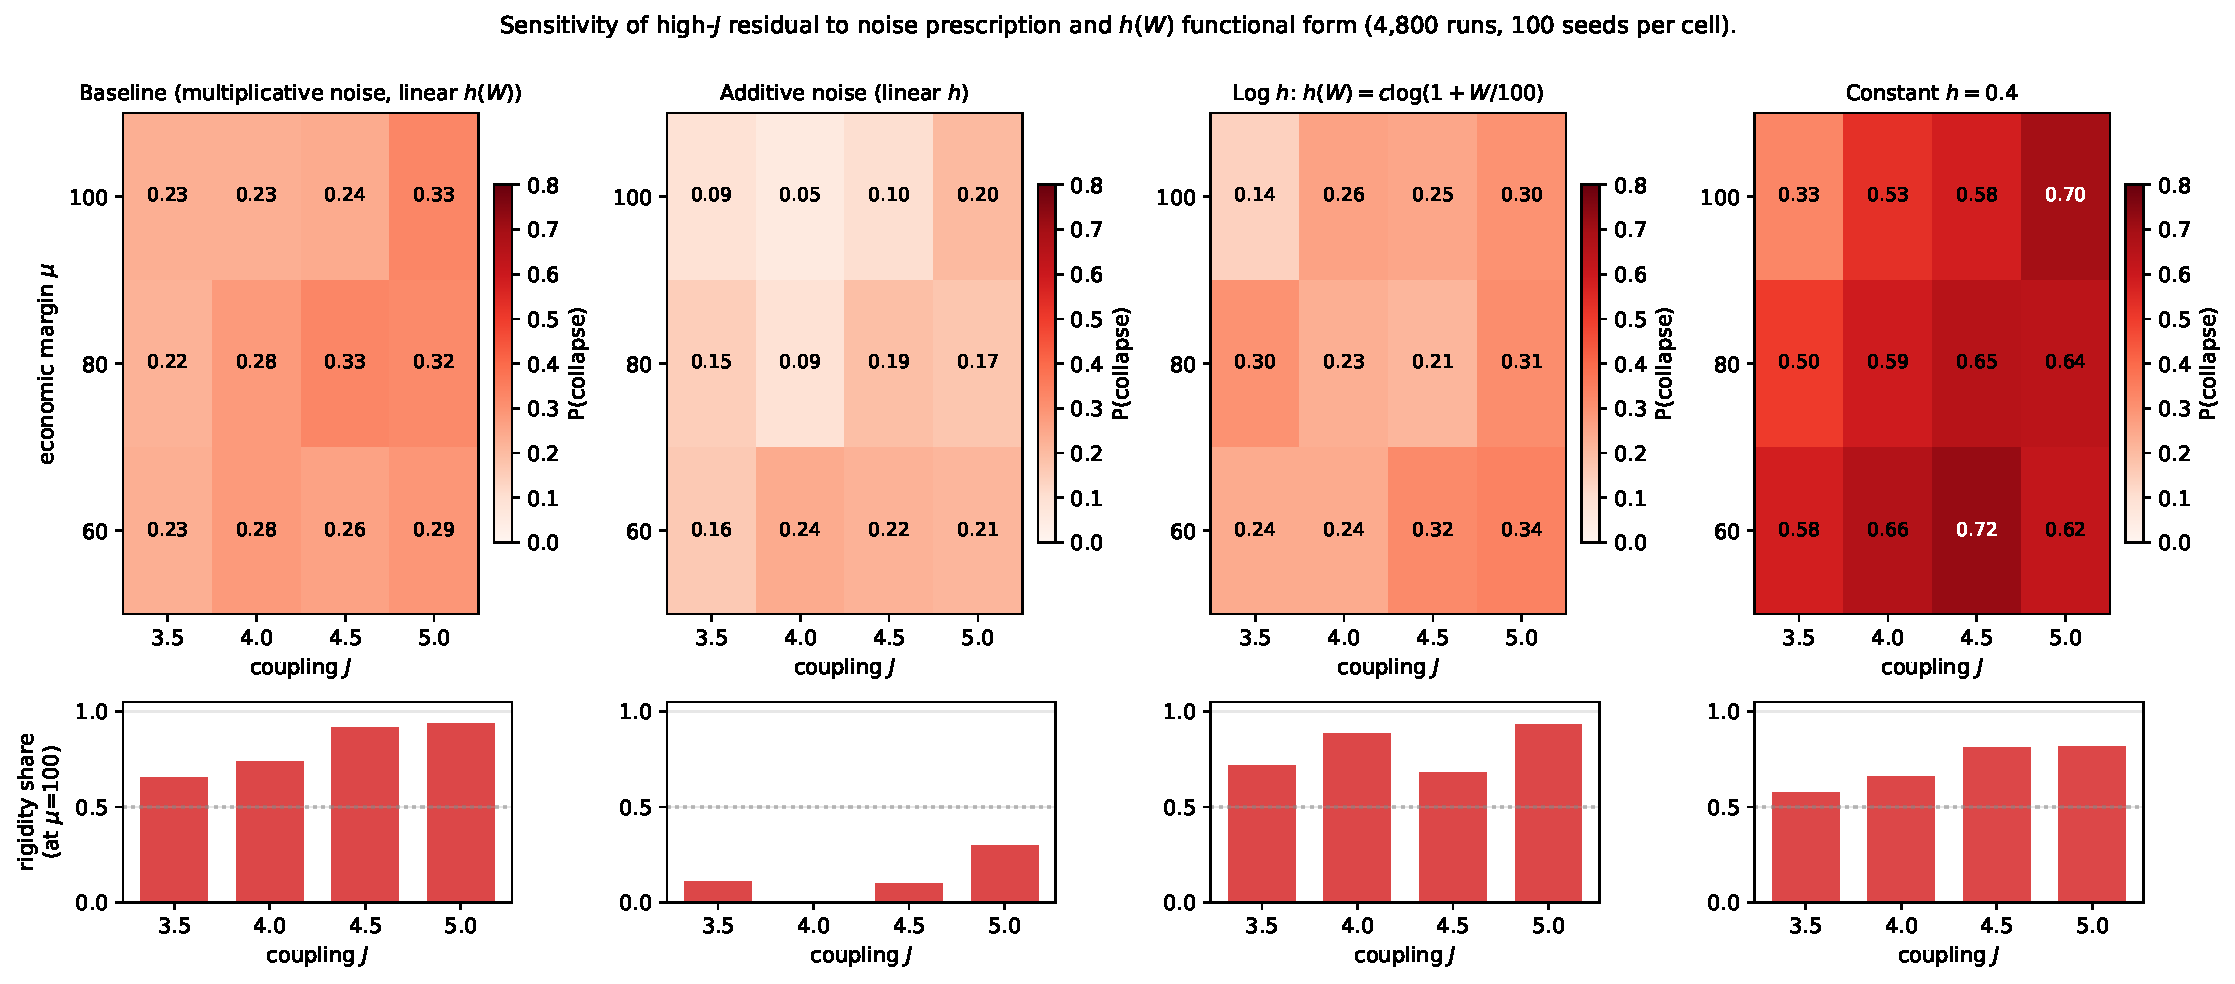
\includegraphics[width=0.95\textwidth]{figures/figS2.pdf}
\caption{\textit{Sensitivity sweep --- noise prescription and h(W) form (supporting §S5.1).} Top row: P(collapse) heatmap over the high-\emph{J} band (\emph{J} ∈ \{3.5, 4, 4.5, 5\}) × protective-margin band (\emph{μ} ∈ \{60, 80, 100\}) for four model variants --- baseline (multiplicative noise \(\xi \sqrt{1-m^2}\), linear \emph{h}(\emph{W}) = 2(\emph{W}/500)), additive noise (constant \emph{ξ}, linear \emph{h}), logarithmic \emph{h}(\emph{W}) = 0.577·log(1+\emph{W}/100), and constant \emph{h} = 0.4. Bottom row: rigidity share at \emph{μ} = 100 across the \emph{J} range for each variant. Headline cell (\emph{J} = 5, \emph{μ} = 100): baseline 0.33, additive 0.20, log \emph{h} 0.30, constant \emph{h} 0.70. The qualitative residual is robust to log-vs-linear \emph{h}; constant \emph{h} is substantially worse, ruling out the baseline as a tuned best-case; under additive noise the residual persists but rigidity-typed dominance falls (0.94 → 0.30; shares under the clipped-EM \textbar{}\emph{m}\textbar{} = 0.9 gate, integrator-scheme caveat of §S4), confirming the rigidity-typed failure signature is multiplicative-noise-specific while the asymmetry itself (and the \emph{h}/\emph{J} landscape result, §S2.5) is not. 4,800 runs total (100 seeds per cell × 12 cells × 4 variants). Source files: \protect\path|simulation/scripts/sensitivity_sweep.py|, \protect\path|simulation/results/sensitivity/figure_s4_sensitivity_sweep.png| (rendered here as Figure S2, \protect\path|manuscript/arxiv/figures/figS2.png|).}
\label{fig:figS2}
\end{figure}



\begin{figure}[H]
\centering
\renewcommand{\figurename}{Supplementary Figure}
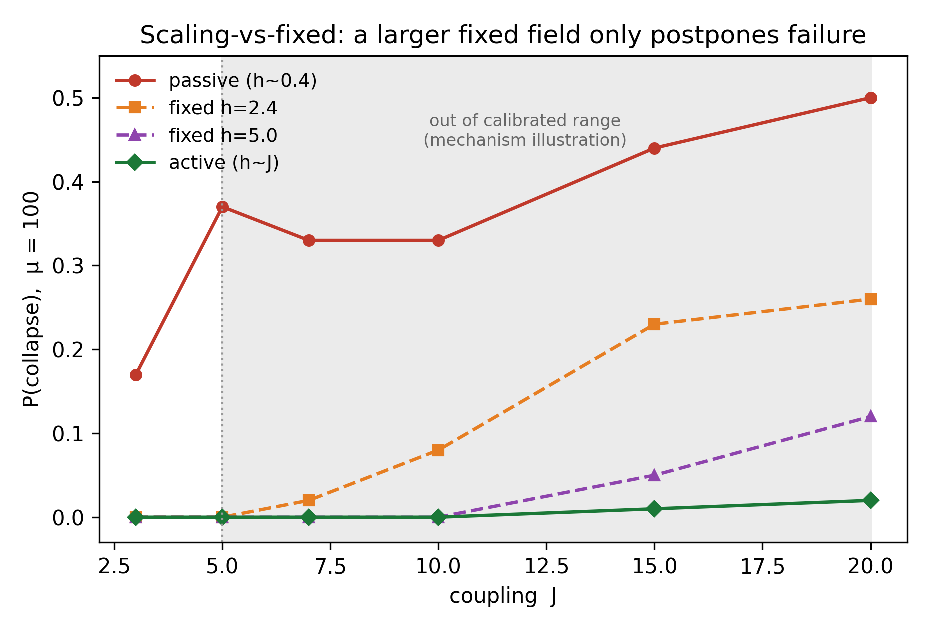
\includegraphics[width=0.95\textwidth]{figures/figS3.pdf}
\caption{\textit{Scaling-vs-fixed control (supporting §S5.1).} P(collapse) at \emph{μ} = 100 vs.~coupling \emph{J} (100 matched seeds) for the passive field (\emph{h} ≈ 0.4), two \emph{fixed} but large fields (\emph{h} = 2.4 and 5.0, the latter 12.5× the initial-wealth baseline field \emph{h}(\emph{W}₀) = 0.4), and the coupling-proportional active field (\emph{h} = 2(\emph{W}/500)·(1 + \emph{J})). A larger \emph{fixed} field only \emph{postpones} failure --- each rises as its tilt-to-barrier ratio \emph{η} = 4\emph{h}/\emph{J} falls (first nonzero failures near \emph{η} ≈ 1.9--2.0 at \emph{n} = 1,000; §S5.1) --- while the coupling-proportional field stays near zero. The shaded region (\emph{J} \textgreater{} 5) is beyond the calibrated range and shown only to expose the mechanism; the fixed-field values there are clipped-EM readings, which the boundary-preserving check of §S4 shows to understate the late-escape channel at \emph{J} ≥ 15 by factors ≈ 1.4--1.6. The contrast is a delivered-magnitude/timing contrast between parameterizations (§S5.6): the coupling-proportional field replenishes \emph{η} by delivering a per-\emph{J} rescaled wealth-fed magnitude, while the fixed fields' \emph{η} decays --- Proposition 1's landscape statement, which motivated the measurement; whether the \emph{η}-decay sets the onset of these failures is open (§S5.8); the late component of the measured fixed-field failures is identified as noise-activated escape (§S9); its weight at the highest couplings remains open. Source: \protect\path|simulation/scripts/scaling_control.py|; figure \protect\path|manuscript/arxiv/figures/figS3.png|.}
\label{fig:figS3}
\end{figure}



\begin{figure}[H]
\centering
\renewcommand{\figurename}{Supplementary Figure}
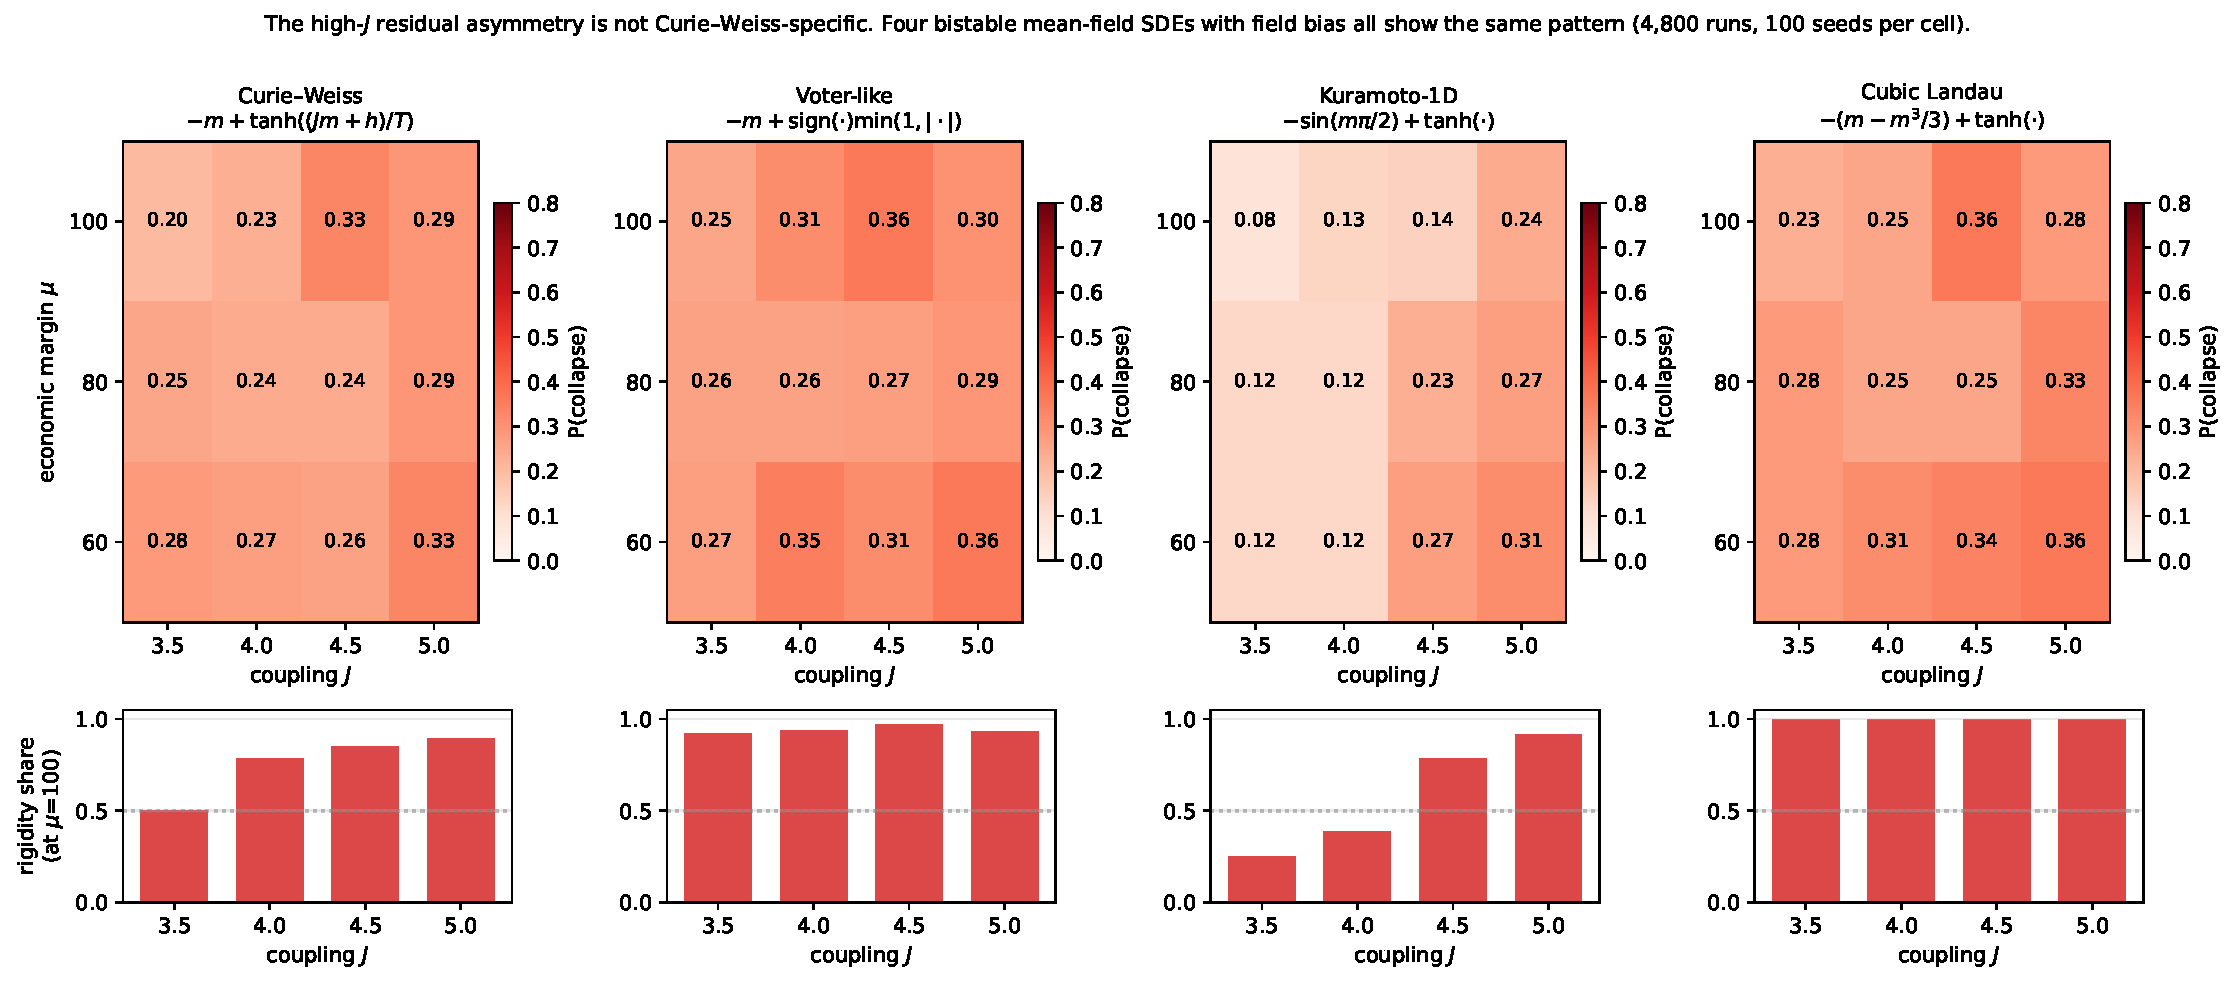
\includegraphics[width=0.95\textwidth]{figures/figS4.pdf}
\caption{\textit{Alternative-model-class robustness (supporting §S5.3).} Top row: P(collapse) heatmap over the high-\emph{J} band (\emph{J} ∈ \{3.5, 4, 4.5, 5\}) × protective-margin band (\emph{μ} ∈ \{60, 80, 100\}) for four bistable mean-field SDEs sharing the field-bias structure but differing in nonlinearity --- Curie--Weiss tanh, voter-like piecewise sign, Kuramoto-1D sine, cubic Landau. Bottom row: rigidity share at \emph{μ} = 100 across the \emph{J} range. At the headline cell (\emph{J} = 5, \emph{μ} = 100): Curie--Weiss 0.29, voter-like 0.30, Kuramoto-1D 0.24, cubic Landau 0.28 --- a 0.24--0.30 band. The high-\emph{J} residual and rigidity-dominance pattern survive across all four model classes (rigidity share at the headline cell is 0.90 / 0.93 / 0.92 / 1.00 respectively; clipped-EM \textbar{}\emph{m}\textbar{} = 0.9 gate, integrator-scheme caveat of §S4), demonstrating that the asymmetry is generic to bistable mean-field SDEs with field bias rather than specific to Curie--Weiss. 4,800 runs total (100 seeds × 12 cells × 4 variants). Source: \protect\path|simulation/results/alternative_class/figure_s5_alternative_class.png| (rendered here as Figure S4, \protect\path|manuscript/arxiv/figures/figS4.png|).}
\label{fig:figS4}
\end{figure}

\begin{center}\rule{0.5\linewidth}{0.5pt}\end{center}

\section{Supplementary Notes}\label{supplementary-notes}

Material moved here from the main text during condensation. Each note carries the full statement whose compressed form appears in the main text; all numbers are unchanged.

\subsection{Note 1 --- Detailed comparison with adjacent recent measurements}\label{note-1-detailed-comparison-with-adjacent-recent-measurements}

Adjacent recent measurements differ in what is measured. A recent preprint studies barrier crossing in a two-dimensional kinetic Ising lattice under heat-bath Monte Carlo with the coupling held fixed (\emph{J} = 1), reporting magnetization distributions, first-passage times, and time-averaged magnetization under bias and stochastic fields \cite{oliverbonafoux2026}; it does not measure a collapse probability as a function of coupling, nor the field amplitude required to hold one fixed. A Research Square preprint treats a McKean--Vlasov mean-field double-well for normative collapse, locating collapse and recovery thresholds and hysteresis-loop properties under a swept control parameter \cite{abreufilho2025}; the measurement in the main text is instead a finite-horizon first-passage probability at fixed parameters under matched-seed stabilizer contrasts, with neither a sweep protocol nor a hysteresis loop. In an applied Ising setting, an enforcement field \emph{h} set against the coupling \emph{J} exhibits the same tension studied here \cite{zaklan2009}, without measuring how the required field amplitude grows with coupling. The bistable coordination structure has economics antecedents beyond the discrete-choice line: multiple search equilibria \cite{diamond1982} and strategic complementarity with multiple equilibria \cite{cooperjohn1988}; the mean-field system measured here is an instance of that coordination-failure structure. None of these works reports a collapse probability as a function of coupling, or the field amplitude required to hold one fixed, under matched-seed stabilizer contrasts.

\subsection{Note 2 --- Note on referents, Definition 1, and noise notation}\label{note-2-note-on-referents-definition-1-and-noise-notation}

\textbf{Note on referents.} Equations 1--2 of the main text constitute a minimal two-variable dynamical system, and the results of the paper are measurements on that system. The words ``wealth'', ``consumption'', and ``subsistence'' are mnemonic labels for the slow feedback variable \emph{W} and its sink terms --- chosen for readability, and consistent with the social-interaction lineage of Equation 1 --- not claims about any empirical economy: no calibration of Equation 2 to data is claimed, and no real-world unit is attached to \emph{W} (the status and sensitivity of the wealth equation are quantified in the main-text Methods and §S5.5). The threshold is chosen as an unambiguously catastrophic event --- a sustained fall to 10\% of initial wealth --- not a transient downturn; mapping it to specific real-world event categories is deferred to future work. The minimal model contains no Hawkes shocks, Lotka--Volterra terms, demographic dynamics, credit cycle, or endogenous beliefs; those enter only at ablation Levels 2--4 (§S1).

\textbf{Definition 1 (formal statement).} A \emph{passive stabilizer} is a mechanism entering the system dynamics whose intervention magnitude is bounded above by a constant independent of the system state and the coupling level. Specifically: (i) its maximum restoring force \emph{h}ₘₐₓ is fixed --- determined by structural parameters alone, not by the current coupling \emph{J}, the current stress level, or the time \emph{t}; (ii) it enters the dynamics as a restoring force favoring a particular equilibrium. An \emph{active stabilizer} is a mechanism whose intervention magnitude is itself a function of the system state, \emph{h} = \emph{g}(\emph{m}, \emph{J}, \emph{t}), with \emph{g} unbounded as stress increases. In Equation 1, \emph{h}(\emph{W}) = 2·(\emph{W}/500) is passive: the wealth-to-force conversion rate is fixed at 2/500 and the field is bounded above by the equilibrium wealth (itself bounded by \emph{μ}). Definition 1 serves as a labeling device for the parameterizations compared in the main text; every conclusion is a measured comparison between fully specified functional forms.

\textbf{Noise notation.} The white-noise process \emph{η}(\emph{t}), always written with its time argument, is distinct from the dimensionless tilt-to-barrier ratio \emph{η} of Proposition 1; §S2.7 writes the same white noise \emph{ζ}(\emph{t}).

\subsection{Note 3 --- Delivered-amplitude controls: full values and caveats}\label{note-3-delivered-amplitude-controls-full-values-and-caveats}

\textbf{Binomial bounds for the matched-seed contrast.} The stress form's P(collapse) = 0.00 across \emph{J} ≥ 4.0 at \emph{μ} = 100 carries a 95\% upper bound of 0.03 per 100-seed cell; where a zero count is reported at \emph{n} = 2,000 the 95\% upper bound is 0.0015, and at \emph{n} = 1,000 it is 0.003 (rule of three; Methods).

\textbf{Delivered equilibrium values (constancy identity).} At the \emph{m} = +1 wealth equilibrium (\emph{W}* = 3,500, base field 14.0) the coupling form delivers 56--294 across \emph{J} = 3--20 and the quadratic form 19.0--238, against the fixed controls' 2.4 and 5.0. There is no within-run \emph{J}-response in the coupling or quadratic variant, so their contrast with the fixed fields is definitionally a delivered-magnitude comparison.

\textbf{Stress-form activation and window-mean control.} The stress form activates its stress term on \textless{} 1.1\% of decision-window seed-steps at α = 2.0, \emph{μ} = 100 (the strong term suppresses the very \emph{m} \textless{} 0 excursions that would activate it); at the informative α = 0.05 the weaker term is active on 22.5--27.8\% of decision-window steps (§S5.6). A constant field matched to its \emph{decision-window} mean (≈5.13--5.24) under-delivers relative to the wealth-fed trajectory over the rest of the run and shows excess collapse at high coupling --- 0.001, 0.021, and 0.057 at \emph{J} = 10, 15, 20 (clipped-EM values at extended \emph{J}, \emph{n} = 2,000). §S4 shows the clipped-EM integrator understates fixed-field failure at \emph{J} ≥ 15, and this control was run under clipped EM only --- it has no boundary-preserving arm.

\textbf{α-sweep summary.} Band-mean residuals are 0.013 (stress) and 0.040 (coupling) at α = 0.5, first reaching 0.00 at the tested α = 1.0, while the quadratic form retains 0.197 at α = 0.5 and reaches 0.00 only at α = 5 (criterion disclosed in §S5.1: band-mean P(collapse) ≤ 0.05 over \emph{J} ∈ \{4.0, 4.5, 5.0\} at \emph{μ} = 100).

\textbf{Extended-\emph{J} per-cell scheme pairs.} For \emph{h} = 2.4, a boundary-preserving paired re-run at \emph{J} = 15 and 20 gives 0.293 and 0.393 against matched clipped-EM arms of 0.183 and 0.247 (\emph{n} = 2,000); for \emph{h} = 5.0 the boundary-preserving paired values are 0.039 and 0.1115 against EM arms 0.0285 and 0.0715. These P(collapse) values are d\emph{t}-converged under both schemes (§S4). The coupling form's per-\emph{J} rescaled field, delivering 224--294 at equilibrium by \emph{J} = 15--20, stays at P ≤ 0.02 throughout (clipped-EM, 100 seeds; §S5.1).

\subsection{Note 4 --- Amplitude requirement: alternative descriptor and overlay detail}\label{note-4-amplitude-requirement-alternative-descriptor-and-overlay-detail}

An alternative two-parameter descriptor that pins the onset at the theoretical value, log \(h_0^*\) = \emph{a} + \emph{p}·log(\emph{J} − 2), fits the §S5.4 data with higher \emph{R}² (0.950--0.997) and near-linear exponents 0.76--1.45, but is not adopted because the free-\(J_{\mathrm{c}}\) fits reject \(J_{\mathrm{c}}\) = 2 in six of eight comparable conditions (§S5.4).

Overlay detail: the theory's in-domain log-log slope is 0.89--0.96 against a measured 1.16--1.93; of the 34 in-domain ratios, 9 deviate by more than 20\%, all within 0.86--1.71. The onset offset has the expected sign because near threshold selection is slow and finite-noise trajectories escape the shallow well anyway, so a larger \emph{J} is needed before a finite \(h_0^*\) is required; no quantitative account is given (§S5.8).

\subsection{Note 5 --- Late channel per-cell detail and ramp profile}\label{note-5-late-channel-per-cell-detail-and-ramp-profile}

\textbf{Late-channel per-cell counts and scheme ranges.} Paired late-collapse counts rise from 75, 127, 11, and 45 (clipped-EM) to 302, 409, 35, and 117 under the boundary-preserving scheme at (\emph{h}, \emph{J}) = (2.4, 15), (2.4, 20), (5.0, 15), (5.0, 20) --- factors of ≈2.6--4 (paired schemes at d\emph{t} = 0.05, \emph{n} = 2,000 per cell). Total P(collapse) in these cells spans the scheme ranges 0.18--0.29, 0.25--0.39, 0.029--0.039, and 0.072--0.112 respectively. Under the boundary-preserving scheme at d\emph{t} = 0.05 the λ ≤ 0 cell medians are 18.7 and 160.5 (the latter dropping to 15.8 at d\emph{t} = 0.025).

\textbf{Ramp-duration profile at the critical margin.} At \emph{μ} = 50 the collapse probability rises from 0.19 at the shortest (1,000-step) ramp through 0.26 and 0.40 to a ≈0.50 plateau (0.51, 0.51, 0.49 at 10,000, 20,000, and 30,000 steps), with the interpolated 50\% crossing at ≈9,200 steps (\texttt{threshold\_by\_mult.csv}). Under sudden onset the per-margin P(collapse) values are 0.47, 0.31, 0.11, 0.14, 0.06, 0.02, 0.02, 0.01, and 0.00 at \emph{μ} = 40, 50, 60, 65, 70, 75, 80, 90, and 100 (\protect\path|simulation/results/dynamic_j/summary.csv|), and the rigidity share of the residual is 77--100\% where \emph{n} ≥ 10 (clipped-EM gate; §S4).

\textbf{Ramp collapse under longer ramps.} Under the dynamic-\emph{J} ramp (\protect\path|simulation/scripts/ramp_speed_sweep.py|; \protect\path|simulation/results/dynamic_j_ramp_speed/summary.csv| and \texttt{raw\_results.csv}), the ramp does not delay collapse near the viability margin: at multiplier 40 the median collapse time is ≈ 21 time units (median collapse step ≈ 414--445) regardless of ramp duration, so the median coupling at the moment of collapse is the schedule read at that early time --- not a ramp effect --- falling from 2.363 (multiplier 40) and 2.858 (multiplier 50) at the shortest (1,000-step) ramp to 0.562 and 0.637 at the longest (30,000-step) ramp, below the deterministic bifurcation \emph{J} = \emph{T} = 2 and barely above the ramp's starting value \emph{J} = 0.5. (At multiplier 50 the median collapse step grows from ≈ 524 to ≈ 915 while the ramp lengthens 30-fold.) The longest-ramp cell at multiplier 40 matches the static (\emph{J} = 0.5, \emph{μ} = 40) cell (P = 1.00). At these longest ramps fragmentation is the largest typed class of collapsed runs (0.54 and 0.51 of collapses at multipliers 40 and 50; the remainder mixed, with rigidity ≤ 0.02; clipped-EM \textbar{}\emph{m}\textbar{} \textless{} 0.3 gate, which carries the scheme caveat of §S4). What triggers these early low-coupling collapses --- as opposed to wealth exhaustion at high coupling --- is left open; the earlier per-run fragment-before-wealth-floor diagnostic is withdrawn because, initialized at \emph{m} = 0, its ordering test fires at the first step and cannot fail.

\subsection{Note 6 --- Boundary, typing, and collapse-definition provenance}\label{note-6-boundary-typing-and-collapse-definition-provenance}

At the headline cell (\emph{J} = 5, \emph{μ} = 100), 0.353 of all trajectory-steps hit the upper boundary and 0.022 the lower. The lower boundary becomes an unattainable \emph{entrance} boundary only for large fixed fields near calibrated \emph{J} (e.g.~\emph{h} = 5.0 at \emph{J} = 5); no boundary is absorbing in any studied regime (§S4). The paired clipped-EM-vs-Lamperti difference in P(collapse) is +0.012 {[}+0.0065, +0.0175{]}. The clipped scheme pins saturated trajectories at exactly 1 − 10⁻⁶ while the reflecting scheme scatters them over ≈{[}0.97, 1{]} --- the origin of the typing-split sensitivity at the \textbar{}\emph{m}\textbar{} = 0.9 gate: 0.88 (0.881) in the \emph{n} = 2,000 paired clipped-EM boundary run vs 0.74 (0.744) under the boundary-preserving integrator, with P(collapse) and timing robust and fragmentation share \textasciitilde0 under both (§S4). Additive noise shifts the balance toward fragmentation: rigidity share 0.94 → 0.30 at the headline cell in the 100-seed noise-variant sweep (clipped-EM gate; §S5.1); the high-\emph{J} orthogonal-variations sweep comprises 4,800 runs (§S5.1). The collapse-definition grid is \emph{W}-threshold ∈ \{5, 10, 20\} × duration ∈ \{100, 200, 400\} steps, and the gate-pair perturbation range is 0.95--0.80 (§S4).

\subsection{Note 7 --- Network extension detail}\label{note-7-network-extension-detail}

The six topologies are complete, Erdős--Rényi, Watts--Strogatz, Barabási--Albert, planted-partition modular, and modular with boundary-only stabilization, under uniform initial condition, uniform field, row-stochastic adjacency, and a shared per-step shock. The apparent spread among the five uniform-field topologies in the 50-seed sweep (0.24--0.34) is independent-seed sampling variation, not a topology effect; the 0.38 endpoint of the full 50-seed spread belongs to the symmetry-breaking modular-boundary variant, which the exact reduction does not cover. ABM sample sizes are \emph{n} = 50--100 (binomial SE ≈ 0.02--0.06); the largest reduction gap, at the pure common-mode endpoint \emph{r} = 1.00, is ABM 0.23 versus scalar 0.314 (≈2 SE). A platform-dependent seed hash was corrected to a stable SHA-1 digest for bit-reproducibility (main-text Methods).

\subsection{Note 8 --- Scope probes: full statement}\label{note-8-scope-probes-full-statement}

Three substrates lie outside the cusp/fold + reversibility criterion for structural reasons, not measurement difficulty: SIR epidemic dynamics (transcritical at \emph{R}₀ = 1, disease-free equilibrium privileged; no bistable cells arose in a broad configuration scan) \cite{vandendriessche2002,hadeler1997}; power-grid cascades (saddle-node, fold not pitchfork) \cite{schaefer2018,manik2017,witthaut2022}; and phase-retrieval neural-network training, where the pilot recorded fold / first-order behaviour with hysteresis (mean hysteresis ≈ 0.75 against the 0.2 threshold) and most tested seeds failed adiabatic reversibility \cite{mannelli2019,mondelli2019}. These do not enter the positive evidence. The one pilot that failed adiabatic reversibility (the neural network) is already excluded by the cusp/fold clause, so the two clauses were not separately tested; the reversibility clause rests on a heuristic.

To complete the map at the cusp + reversible corner the degenerate optical parametric oscillator (DOPO) was tested --- the canonical ℤ₂-symmetric pitchfork and physical basis of coherent Ising machines \cite{drummond1980,drummond1981,wang2013cim,marandi2014}. Pilot measurements, pre-specified (protocol archived in the code repository and the Zenodo archive), confirmed the near-cusp field exponent, excluding the fold value, and matched the parameter-free near-threshold coefficient; the mean cross-barrier time rises monotonically with the pump above threshold, and the DOPO passed the same adiabatic-reversibility test that most neural-network seeds failed. The pre-specified, secondary, confirmatory-only deep-well coupling-exponent test was inconclusive at the achieved precision and cannot separate the corrected from the original exponent. DOPO is a deliberately engineered cusp; its role is corner-completion of the scope-criterion map --- a high-confidence confirmation of the cusp + reversible corner, with low could-fail value --- not a risky falsification test.

The mean-field idealization is not an approximation for the network configuration tested: under a common-mode shock with a uniform stabilizer field, the \emph{N}-agent system on any row-stochastic topology reduces exactly to the one-dimensional SDE (§S6), so the network extension tests the noise-composition scope condition, not topology. The one variant in which agents differentiate (boundary-only stabilization) is not separated from the uniform-field value at the tested sample sizes.

\section{Late-channel mechanism: noise-activated escape}\label{late-channel-mechanism-noise-activated-escape}

This section reports the tests that identify the late collapse channel as noise-activated (Kramers) escape from the metastable well, a process distinct from the early transient branch selection. The tests, cells, and pass/fail thresholds were fixed in advance in a pre-registration committed before the results existed (\protect\path|simulation/prereg/PRESPEC_late_channel_mechanism_2026-08-22.md|); the generating script is \protect\path|simulation/scripts/late_channel_mechanism.py| and outputs are under \protect\path|simulation/results/late_channel_mechanism/|.

All runs use the boundary-preserving (constant-diffusion Lamperti) integrator with constant field \emph{h} and the identical wealth/collapse ledger as §S4, at d\emph{t} = 0.05, 20,000 steps (\(t_{\max}\) = 1,000), \emph{T} = 2, ξ = 0.5, \emph{μ} = 100, \emph{W}₀ = 100, \emph{n} = 2,000 per cell, over \emph{h} ∈ \{2.4, 5.0\} × \emph{J} ∈ \{7, 10, 15, 20\}. Early collapses are those with collapse time \emph{t} ≤ 50; late collapses \emph{t} \textgreater{} 250. The late-escape hazard \emph{r} is the maximum-likelihood constant rate in the window (250, 1,000{]}, i.e.~late collapses divided by person-time at risk after \emph{t} = 250 among trajectories uncollapsed at \emph{t} = 250.

The timing separation of the two channels (main text, ``The late channel'') is: the wealth-fed baseline collapses are purely early (medians 14.7--17.0 across \emph{J} = 2.5--5, all by \emph{t} = 42, zero after \emph{t} = 100), whereas the fixed-field failures are a mixture with passive-like medians 14.2--14.5 alongside the late tail (8--28\% after \emph{t} = 100, 99th percentiles ≈779--985; clipped EM, \emph{n} = 1,000).

For reference, under this integrator the late channel strengthens relative to clipped Euler--Maruyama (paired late-collapse counts rise by ≈2.6--4× across the four failing (\emph{h}, \emph{J}) cells and the late fraction of collapses rises from 0.19--0.32 to 0.45--0.53 at d\emph{t} = 0.05); P(collapse) is d\emph{t}-converged in all eight scheme×cell checks, while the late-fraction share at \emph{J} = 20 is not, shrinking ≈8--13 percentage points at d\emph{t} = 0.025 (§S4). The late-channel \emph{weight} at the highest couplings therefore remains open; the mechanism tests below concern the \emph{rate}, which is well defined regardless of the weight.

\subsection{Test 1 --- initial-condition dependence (decisive)}\label{test-1-initial-condition-dependence-decisive}

Each cell is run from two initial conditions on the same seed stream: (a) \emph{m}₀ = 0 (disordered start; both channels can operate), and (b) \emph{m}₀ = +0.9 (deep in the protected well; branch selection cannot operate). If the late channel is activated escape from the well, IC (b) should remove the early collapses while preserving the late-escape rate; if the late collapses are instead slow stragglers of the same selection transient, they should vanish along with the early ones.

{\def\LTcaptype{none} % do not increment counter
\begin{longtable}[]{@{}
  >{\raggedright\arraybackslash}p{(\linewidth - 12\tabcolsep) * \real{0.1429}}
  >{\raggedright\arraybackslash}p{(\linewidth - 12\tabcolsep) * \real{0.1429}}
  >{\raggedright\arraybackslash}p{(\linewidth - 12\tabcolsep) * \real{0.1429}}
  >{\raggedright\arraybackslash}p{(\linewidth - 12\tabcolsep) * \real{0.1429}}
  >{\raggedright\arraybackslash}p{(\linewidth - 12\tabcolsep) * \real{0.1429}}
  >{\raggedright\arraybackslash}p{(\linewidth - 12\tabcolsep) * \real{0.1429}}
  >{\raggedright\arraybackslash}p{(\linewidth - 12\tabcolsep) * \real{0.1429}}@{}}
\toprule\noalign{}
\begin{minipage}[b]{\linewidth}\raggedright
\emph{h}
\end{minipage} & \begin{minipage}[b]{\linewidth}\raggedright
\emph{J}
\end{minipage} & \begin{minipage}[b]{\linewidth}\raggedright
IC
\end{minipage} & \begin{minipage}[b]{\linewidth}\raggedright
P(collapse)
\end{minipage} & \begin{minipage}[b]{\linewidth}\raggedright
early (\emph{t}≤50)
\end{minipage} & \begin{minipage}[b]{\linewidth}\raggedright
late (\emph{t}\textgreater250)
\end{minipage} & \begin{minipage}[b]{\linewidth}\raggedright
late rate \emph{r} (per unit \emph{t})
\end{minipage} \\
\midrule\noalign{}
\endhead
\bottomrule\noalign{}
\endlastfoot
2.4 & 7 & \emph{m}₀=0 & 0.024 & 38 & 7 & 4.8×10⁻⁶ \\
2.4 & 7 & \emph{m}₀=+0.9 & 0.004 & 2 & 5 & 3.3×10⁻⁶ \\
2.4 & 10 & \emph{m}₀=0 & 0.137 & 141 & 111 & 8.3×10⁻⁵ \\
2.4 & 10 & \emph{m}₀=+0.9 & 0.078 & 2 & 126 & 8.8×10⁻⁵ \\
2.4 & 15 & \emph{m}₀=0 & 0.294 & 282 & 245 & 2.13×10⁻⁴ \\
2.4 & 15 & \emph{m}₀=+0.9 & 0.202 & 11 & 314 & 2.40×10⁻⁴ \\
2.4 & 20 & \emph{m}₀=0 & 0.413 & 366 & 372 & 3.65×10⁻⁴ \\
2.4 & 20 & \emph{m}₀=+0.9 & 0.279 & 15 & 437 & 3.52×10⁻⁴ \\
5.0 & 7 & \emph{m}₀=0 & 0.000 & 0 & 0 & 0 \\
5.0 & 7 & \emph{m}₀=+0.9 & 0.000 & 0 & 0 & 0 \\
5.0 & 10 & \emph{m}₀=0 & 0.0005 & 1 & 0 & 0 \\
5.0 & 10 & \emph{m}₀=+0.9 & 0.000 & 0 & 0 & 0 \\
5.0 & 15 & \emph{m}₀=0 & 0.040 & 45 & 28 & 1.93×10⁻⁵ \\
5.0 & 15 & \emph{m}₀=+0.9 & 0.017 & 1 & 28 & 1.89×10⁻⁵ \\
5.0 & 20 & \emph{m}₀=0 & 0.098 & 82 & 88 & 6.35×10⁻⁵ \\
5.0 & 20 & \emph{m}₀=+0.9 & 0.059 & 1 & 97 & 6.70×10⁻⁵ \\
\end{longtable}
}

Pooled across cells, starting deep in the well removes 96.6\% of early collapses (955 → 32) while the pooled late hazard is preserved (ratio \emph{r}(b)/\emph{r}(a) = 1.12). The per-cell hazard ratios, for cells with ≥ 10 late collapses in both arms, are 1.06, 1.13, 0.97, 0.98, and 1.05 --- all within the pre-declared factor-of-two band and clustered at unity. The late-escape rate is thus independent of how the well was reached, the defining property of activated escape and the pre-declared decisive criterion (supported). The initial-condition-independent constant hazard is also the memoryless (Poisson) signature that Test 3 could not measure directly (below).

\subsection{Test 2 --- barrier (Arrhenius) scaling and noise dependence}\label{test-2-barrier-arrhenius-scaling-and-noise-dependence}

For each cell the deterministic drift \emph{f}(\emph{m}) = −\emph{m} + tanh((\emph{Jm} + \emph{h})/\emph{T}) has a stable high-\emph{m} well \(m_+\) and an unstable saddle \(m_s\). Two barriers are computed: the drift-potential barrier \(\Delta U = U(m_s) - U(m_+)\) with \(U(m) = \int [m - \tanh((Jm+h)/T)]\,\mathrm{d}m\), and the multiplicative-noise geometric barrier \(G = \int_{m_s}^{m_+} f/(1-m^2)\,\mathrm{d}m\), for which the Itô stationary theory gives escape rate \(r \propto \exp(-(2/\xi^2)\,G)\).

{\def\LTcaptype{none} % do not increment counter
\begin{longtable}[]{@{}lllllll@{}}
\toprule\noalign{}
\emph{h} & \emph{J} & \(m_s\) & Δ\emph{U} & \emph{G} & late rate \emph{r} & ln \emph{r} \\
\midrule\noalign{}
\endhead
\bottomrule\noalign{}
\endlastfoot
2.4 & 10 & −0.302 & 0.638 & 0.833 & 8.3×10⁻⁵ & −9.39 \\
2.4 & 15 & −0.185 & 0.582 & 0.776 & 2.13×10⁻⁴ & −8.45 \\
2.4 & 20 & −0.133 & 0.559 & 0.752 & 3.65×10⁻⁴ & −7.92 \\
5.0 & 15 & −0.388 & 0.805 & 1.009 & 1.93×10⁻⁵ & −10.85 \\
5.0 & 20 & −0.279 & 0.715 & 0.912 & 6.35×10⁻⁵ & −9.66 \\
\end{longtable}
}

Across the five cells with ≥ 10 late collapses, ln \emph{r} is linear in Δ\emph{U} (slope −10.98, \emph{R}² = 0.953) and in \emph{G} (slope −10.55, \emph{R}² = 0.953). Kramers with multiplicative noise predicts a \emph{G}-slope of −2/ξ² = −8.0; the fitted −10.55 is within the pre-declared ±40\% band ({[}−11.2, −4.8{]}). The ≈30\% overshoot is consistent with the finite-barrier and prefactor corrections not captured by the leading-exponential estimate. A noise sweep at (\emph{h} = 2.4, \emph{J} = 15) confirms the direction: the late hazard is 0 (0 late collapses), 2.13×10⁻⁴, and 9.3×10⁻⁴ at ξ = 0.35, 0.50, 0.65 --- monotonically increasing as the effective barrier 2\emph{G}/ξ² (12.67, 6.21, 3.67) falls.

\textbf{Monostable control.} At (\emph{h} = 5.0, \emph{J} = 7) the drift is monostable --- the only fixed point is the high-\emph{m} well, with no saddle and hence no barrier to cross --- and the observed late-collapse count is exactly zero (P(collapse) = 0.000, both initial conditions). This is consistent with activated escape, though not uniquely diagnostic of it: the bistable (\emph{h} = 5.0, \emph{J} = 10) cell, whose barrier is large (2\emph{G}/\emph{ξ}² ≈ 10.2), also yields zero late collapses in the observation window, as an Arrhenius rate suppressed by that barrier predicts. The monostable zero therefore corroborates, rather than establishes, the escape picture; the initial-condition independence of Test 1 remains the decisive evidence.

\subsection{Test 3 --- waiting-time distribution (underpowered by truncation)}\label{test-3-waiting-time-distribution-underpowered-by-truncation}

The pre-registration also specified a memorylessness test: pooled late waiting times should be exponential (coefficient of variation CV ≈ 1, KS not rejecting an exponential at \emph{p} \textgreater{} 0.05). This test failed its threshold --- the late collapse-time and \emph{m}-escape-time series have CV ≈ 0.56--0.68 and KS rejects the plain exponential (\emph{p} \textless{} 0.05 in 10 of 11 scored series; the remaining series, the (\emph{h} = 5.0, \emph{J} = 15) collapse times at \emph{n} = 28, has \emph{p} = 0.112). The failure is a diagnostic-design limitation, not evidence against escape: the mean escape time 1/\emph{r} is 2,700--52,600 time units while the observation window after \emph{t} = 250 is only 750, so only the first 1--27\% of the exponential is visible. Right-truncation of an exponential to a window short compared with its mean drives the CV toward the uniform-front value 1/\(\sqrt{3}\) ≈ 0.577, which is what is observed. The test is therefore underpowered rather than contradictory; the constant, initial-condition-independent hazard established in Test 1 is the operative memorylessness signature. Measuring CV ≈ 1 directly would require running the horizon to a multiple of 1/\emph{r} (tens of thousands of time units), which is deferred.


\bibliographystyle{unsrtnat}
\bibliography{references}

\end{document}
